\documentclass[11pt,a4paper]{article}

\usepackage[margin=2.2cm]{geometry}
\usepackage[T1]{fontenc}
\usepackage[utf8]{inputenc}
\usepackage{lmodern}
\usepackage{microtype}
\usepackage{amsmath,amssymb}
\usepackage{graphicx}
\usepackage{booktabs}
\usepackage{enumitem}
\usepackage{xcolor}
\usepackage{listings}
\usepackage{caption}
\usepackage{float}
\usepackage[most]{tcolorbox}
\usepackage{fancyhdr}
\usepackage{tikz}
\usepackage{cancel}
\usepackage[hidelinks]{hyperref}

\definecolor{markred}{RGB}{217,13,13}
\definecolor{codebg}{RGB}{245,245,245}

\newcommand{\btn}[1]{\fbox{\small\textsf{#1}}}                 % a button of the GUI
\newcommand{\ctl}[1]{\textsf{#1}}                              % a slider / toggle label
\newcommand{\step}[1]{\tikz[baseline=(c.base)]\node[circle,fill=markred,text=white,inner sep=1.2pt,font=\bfseries\small](c){#1};}
\newcommand{\file}[1]{\texttt{#1}}
\newcommand{\dd}{\mathrm{d}}
\newcommand{\vth}{\boldsymbol{\theta}}
\newcommand{\vp}{\mathbf{p}}
\newcommand{\vd}{\mathbf{d}}

\newtcolorbox{tryit}{colback=blue!3,colframe=blue!45!black,title=Things to try,fonttitle=\bfseries,
  left=4pt,right=4pt,top=3pt,bottom=3pt}
\newtcolorbox{note}[1][Note]{colback=yellow!6,colframe=orange!70!black,title=#1,fonttitle=\bfseries,
  left=4pt,right=4pt,top=3pt,bottom=3pt}
\newtcolorbox{keypoint}{colback=green!4,colframe=green!40!black,title=Key point,fonttitle=\bfseries,
  left=4pt,right=4pt,top=3pt,bottom=3pt}

\lstdefinelanguage{julia}{
  morekeywords={function,end,for,in,if,else,elseif,return,using,const,struct,include,let,do},
  sensitive=true, morecomment=[l]{\#}, morestring=[b]"}
\lstset{language=julia, basicstyle=\ttfamily\small, backgroundcolor=\color{codebg},
  keywordstyle=\color{blue!60!black}\bfseries, commentstyle=\color{green!40!black},
  stringstyle=\color{red!60!black}, frame=single, rulecolor=\color{black!20},
  columns=fullflexible, keepspaces=true, showstringspaces=false, xleftmargin=4pt, xrightmargin=4pt,
  literate={–}{{--}}1 {·}{{$\cdot$}}1 {θ}{{$\theta$}}1 {χ}{{$\chi$}}1 {²}{{$^2$}}1}

\pagestyle{fancy}
\fancyhf{}
\lhead{\small Bayesian inversion with MCMC and HMC in Julia}
\rhead{\small\thepage}
\renewcommand{\headrulewidth}{0.3pt}

\setlist{itemsep=2pt,topsep=4pt}
\captionsetup{font=small,labelfont=bf}

\title{\textbf{Bayesian inversion with Markov chain Monte Carlo in Julia}\\[4pt]
\large A guide to seven interactive programs: Metropolis, Metropolis--Hastings,\\ Hamiltonian Monte Carlo and two comparisons}
\author{Evangelos Moulas\\[2pt] {\small (made using Claude)}}
\date{Version 1.0 -- 15 Nov.\ 2026}

\begin{document}
\maketitle
\vspace{-3ex}
\thispagestyle{empty}

\begin{abstract}
\noindent Fitting a model to noisy data gives more than a ``best'' parameter value: Bayes' theorem turns the
data, the noise and our prior knowledge into a probability distribution of the parameters, the
\emph{posterior}. In practice the posterior is known only up to a normalising integral that cannot be computed
when there are more than a few parameters. Markov chain Monte Carlo (MCMC) methods avoid this integral: they
draw samples from the posterior using only \emph{ratios} of posterior values, in which the integral cancels.
This guide explains seven interactive Julia programs that let you watch these samplers at work on the simplest
possible inverse problem, fitting a straight line to noisy data. Programs 1--3 introduce the Metropolis and
Metropolis--Hastings algorithms (one and two parameters), Programs 4--5 Hamiltonian Monte Carlo (HMC), and
Program 6 runs both kinds of sampler side by side to see which converges faster; Program 7 repeats the comparison
for a polynomial with up to ten parameters, to see how the two methods behave when the number of parameters grows.
Section~\ref{sec:intro} explains how to start the programs, Sections~\ref{sec:bayes}--\ref{sec:numerics}
summarise the theory and the numerics, and Sections~\ref{sec:m1}--\ref{sec:cmp2} go through the programs one by
one. Every program has an annotated screenshot: the red numbers \step{1}, \step{2}, \dots\ show where to click
and in which order.
\end{abstract}

\vspace{-2ex}
\tableofcontents
\newpage

%==============================================================================
\section{Introduction and installation}\label{sec:intro}
%==============================================================================

\subsection{What the programs do}
All programs fit a straight line to synthetic data that you generate yourself: you choose the true parameters
and the noise level, the program adds random noise, and a sampler then tries to recover the parameters
\emph{together with their uncertainty}. Because the true answer is known (for a straight line with Gaussian
noise and a Gaussian prior the posterior can even be computed exactly), you can always check whether a sampler
works and how fast it gets there.

\begin{table}[H]
\centering\footnotesize\setlength{\tabcolsep}{4pt}
\caption{The programs. All of them are in the main folder \file{julia\_MCMC}.}\label{tab:files}
\begin{tabular}{@{}llll@{}}
\toprule
& File & Model & Sampler \\
\midrule
1 & \file{Introduction\_MCMC\_1.jl}        & $y=k\,x$     & Metropolis (random walk) \\
2 & \file{Introduction\_MCMC\_2.jl}        & $y=k\,x$     & Metropolis--Hastings, four proposals, Hastings correction on/off \\
3 & \file{Introduction\_MCMC\_3.jl}        & $y=a+k\,x$   & Metropolis--Hastings in two dimensions, learned proposal covariance \\
4 & \file{Introduction\_HMC\_1.jl}         & $y=k\,x$     & Hamiltonian Monte Carlo, phase space $(k,p)$ \\
5 & \file{Introduction\_HMC\_2.jl}         & $y=a+k\,x$   & HMC in two dimensions, mass matrix, jitter \\
6 & \file{Comparison\_MCMC\_to\_HMC\_1.jl} & $y=a+k\,x$   & Metropolis and HMC side by side \\
7 & \file{Comparison\_MCMC\_to\_HMC\_2.jl} & polynomial   & both side by side for $D=1\dots10$ parameters \\
\midrule
& \file{Project.toml}, \file{Manifest.toml} & -- & the Julia packages (GLMakie, LinearAlgebra, \dots) \\
& \file{guide/}                               & -- & this guide and the program that makes its screenshots \\
\bottomrule
\end{tabular}
\end{table}

\subsection{Installation (once)}
\begin{enumerate}
\item Install a recent Julia from \url{https://julialang.org/downloads/} (the package versions in
  \file{Manifest.toml} were resolved with Julia 1.13; with an older Julia, \lstinline{Pkg.instantiate()} may
  have to resolve them again). The recommended installer is \emph{juliaup}; on Windows install
  \emph{Julia} from the Microsoft Store, on macOS/Linux type in a terminal
\begin{lstlisting}
curl -fsSL https://install.julialang.org | sh
\end{lstlisting}
\item Copy the folder \file{julia\_MCMC} to your computer.
\item Open a terminal in that folder and install the packages listed in \file{Project.toml}:
\begin{lstlisting}
julia --project=. -e "using Pkg; Pkg.instantiate()"
\end{lstlisting}
  This downloads and precompiles GLMakie (interactive graphics) and takes a few minutes the first time.
  The programs in the folders \file{julia\_Legendre} and \file{julia\_interactive\_thermo} use the same
  package versions; if you already use them, nothing new has to be downloaded.
\end{enumerate}

\subsection{Running a program}
From a terminal in the folder:
\begin{lstlisting}
julia Introduction_MCMC_1.jl
\end{lstlisting}
or from the Julia REPL: \lstinline{include("Introduction_MCMC_1.jl")}. Every program activates its own
environment (\lstinline{Pkg.activate(@__DIR__)}), so you do not have to start Julia with
\lstinline{--project}. A window opens; when the program was started from a terminal, it keeps running until
the window is closed.

\begin{note}
The first start of a Julia session is slow (loading and compiling GLMakie, about 30--60\,s). Starting from
the REPL and \lstinline{include}-ing the programs one after the other avoids paying this time again.
The window adapts to its size; on a small screen the data panel (upper left) becomes smaller first, the
controls always stay visible.
\end{note}

\subsection{Elements of the user interface}
All programs share the same layout: the \textbf{data} in the upper left, the \textbf{controls} below it, the
\textbf{misfit} (or the misfit map) in the upper right and the \textbf{posterior and trace plots} in the lower
right.
\begin{itemize}
\item \textbf{Data sliders} (true parameters, noise $\sigma$, number of points $N$) take effect only when
  \btn{Initialise data} is pressed; until then the status line reminds you in red. \btn{new noise realisation}
  draws new $x$ positions and new noise. The noise values are kept between initialisations, so changing $\sigma$
  only rescales the same noise.
\item \textbf{Prior and starting point.} Changing the prior changes the target distribution; changing the
  starting point changes the chain. Both restart the chain. A left click in the misfit panel (or map) sets
  the starting point.
\item \textbf{Run}: each press adds a \emph{batch} of 1, 10, 100 or 1000 iterations (slider
  \ctl{batch size}). With a batch of 1 the last step is explained in detail: the proposal, the acceptance
  probability $\alpha$ and the random number $u$ that decided. \btn{Reset chain} starts again at the starting
  point.
\item \ctl{burn-in}: the first iterations that are discarded from the statistics (grey band in the trace
  plot).
\item \textbf{Toggles} switch display elements on and off; \ctl{zoom on posterior} zooms all parameter axes
  to $\pm 6$ (two parameters: $\pm4.5$) posterior standard deviations around the exact posterior mean.
\item The \textbf{info text} below the controls lists the number of iterations, the acceptance rate, the
  sample mean and standard deviation (after burn-in) and the exact posterior for comparison.
\end{itemize}
Colours are used consistently: data black, true values grey dashed, the current state of the chain orange,
visited states and the sample histogram green, rejected proposals red, the prior blue, the exact posterior
black dashed.

%==============================================================================
\section{Bayes' theorem: why we need Bayesian statistics}\label{sec:bayes}
%==============================================================================

\subsection{Forward and inverse problems}
A \emph{forward problem} predicts data from parameters: given the slope $k$ of a line, the model
$g(x;k)=k\,x$ predicts $y$ at every $x$. Most questions in the Earth sciences are \emph{inverse problems}: we
measure data $\vd=(y_1,\dots,y_N)$ and want to learn the parameters $\vth$ (a slope; or a pressure and a
temperature from mineral compositions; or a time scale from a diffusion profile). Measured data are noisy,
\begin{equation}
  y_i = g(x_i;\vth_\text{true}) + \varepsilon_i ,\qquad \varepsilon_i \sim \mathcal{N}(0,\sigma^2),
  \label{eq:data}
\end{equation}
so many parameter values explain the data almost equally well. The question is therefore not only ``which
$\vth$ fits best?'' but ``which values of $\vth$ are compatible with the data, and how probable is each of
them?''

\subsection{Bayes' theorem}
Probability theory answers this question with two rules. The joint probability of parameters and data can be
written in two ways (product rule),
\begin{equation}
  p(\vth,\vd) = p(\vd\,|\,\vth)\,p(\vth) = p(\vth\,|\,\vd)\,p(\vd),
\end{equation}
and solving for $p(\vth|\vd)$ gives \textbf{Bayes' theorem}:
\begin{equation}
  \boxed{\;p(\vth\,|\,\vd) \;=\; \frac{p(\vd\,|\,\vth)\;p(\vth)}{p(\vd)}\;},\qquad
  p(\vd) = \int p(\vd\,|\,\vth)\,p(\vth)\,\dd\vth .
  \label{eq:bayes}
\end{equation}
\begin{itemize}
\item $p(\vth)$, the \textbf{prior}: what we know about the parameters \emph{before} the measurement (physical
  limits, earlier experiments, a rough guess). In the programs it is a Gaussian $\mathcal{N}(\mu_p,\sigma_p^2)$.
\item $p(\vd|\vth)$, the \textbf{likelihood}: how probable the measured data are if the parameters were $\vth$.
  It contains the forward model and the noise model.
\item $p(\vth|\vd)$, the \textbf{posterior}: what we know \emph{after} the measurement. This is the answer of a
  Bayesian inversion: a probability distribution, not a single number.
\item $p(\vd)$, the \textbf{evidence} (or marginal likelihood): the integral of the numerator over all
  parameters. It does not depend on $\vth$; it only normalises the posterior so that it integrates to one.
\end{itemize}

\subsection{Gaussian noise: the likelihood and the misfit $\chi^2$}
For independent Gaussian noise \eqref{eq:data} the likelihood is a product of Gaussians,
\begin{equation}
  p(\vd\,|\,\vth) = \prod_{i=1}^{N} \frac{1}{\sqrt{2\pi}\,\sigma}\,
     \exp\!\Bigl(-\frac{(y_i-g(x_i;\vth))^2}{2\sigma^2}\Bigr)
  \;\propto\; \exp\!\Bigl(-\tfrac12\chi^2(\vth)\Bigr),\qquad
  \chi^2(\vth) = \sum_{i=1}^{N}\frac{\bigl(y_i-g(x_i;\vth)\bigr)^2}{\sigma^2}.
  \label{eq:chi2}
\end{equation}
$\chi^2$ is the familiar \emph{misfit} of least squares, and the posterior is
\begin{equation}
  p(\vth\,|\,\vd) \;\propto\; \exp\!\Bigl(-\tfrac12\chi^2(\vth)\Bigr)\;p(\vth).
  \label{eq:post}
\end{equation}
The minimum of $\chi^2$ (the least-squares fit) is the maximum of the likelihood. Least squares thus finds the
top of the posterior (for a flat prior), but it does not tell us how wide the posterior is, whether it is
skewed, whether it has several maxima, or how the parameters are correlated.

\subsection{Why Bayesian statistics?}
\begin{itemize}
\item \textbf{The answer is a distribution.} Uncertainties, confidence intervals and correlations between
  parameters follow directly from the posterior; no separate error propagation is needed. In
  Program~3 you will see that the slope and the intercept of a line are strongly anti-correlated, something a
  ``best fit $\pm$ error bar'' for each parameter does not show.
\item \textbf{Prior knowledge enters explicitly.} Physical limits (a temperature is positive, a fraction lies
  between 0 and 1) or results of earlier studies are part of the calculation and are stated openly, instead of
  being hidden in the choice of a starting value or in ad-hoc constraints.
\item \textbf{Non-linear models.} For non-linear forward models (thermodynamic equilibria, diffusion,
  kinetics) the posterior can be curved, skewed or have several maxima; linearised error propagation then fails,
  the posterior does not.
\item \textbf{Nuisance parameters} that are needed by the model but not of interest are simply integrated out
  (marginalisation): $p(\theta_1|\vd)=\int p(\theta_1,\theta_2|\vd)\,\dd\theta_2$.
\item \textbf{Predictions with uncertainty.} Every posterior sample is a model that fits the data; drawing the
  model of many samples (the thin green lines in the data panel of the programs) shows the uncertainty of a
  prediction.
\end{itemize}

\subsection{The problem: integrals}\label{sec:integrals}
Everything we want to know from the posterior is an integral: its normalisation $p(\vd)$ in \eqref{eq:bayes},
the posterior mean $\int\vth\,p(\vth|\vd)\,\dd\vth$, the variances, the marginal distributions, the
probability that a parameter exceeds a threshold. With one or two parameters these integrals can be computed on
a grid. With $D$ parameters and 100 grid points per parameter the grid has $100^D$ points: $10^{20}$ for
$D=10$, far beyond any computer.

The way out is \textbf{Monte Carlo integration}: if we had $n$ samples $\vth_1,\dots,\vth_n$ drawn from the
posterior, every integral would become an average,
\begin{equation}
  \int f(\vth)\,p(\vth\,|\,\vd)\,\dd\vth \;\approx\; \frac1n\sum_{j=1}^{n} f(\vth_j),
  \label{eq:mc}
\end{equation}
with an error that decreases as $1/\sqrt{n}$ \emph{independently of the number of parameters}. Histograms of
the samples are the marginal distributions. The remaining problem is how to draw samples from a distribution
that we know only up to its normalisation $p(\vd)$, which is exactly the integral we cannot compute. This is
what Markov chain Monte Carlo does.

\subsection{The example of the programs}\label{sec:example}
Programs 1, 2 and 4 fit the line through the origin $y=k\,x$ (one parameter), Programs 3, 5 and 6 the line
$y=a+k\,x$ (intercept $a$, slope $k$). With Gaussian priors $k\sim\mathcal{N}(\mu_k,\sigma_k^2)$,
$a\sim\mathcal{N}(\mu_a,\sigma_a^2)$ the logarithm of the posterior \eqref{eq:post} is a quadratic function of
the parameters, so the posterior is an exact Gaussian. For one parameter
\begin{equation}
  \frac{1}{\sigma_\text{post}^2} = \frac{\sum x_i^2}{\sigma^2} + \frac{1}{\sigma_p^2},\qquad
  k_\text{post} = \sigma_\text{post}^2\Bigl(\frac{\sum x_i y_i}{\sigma^2} + \frac{\mu_p}{\sigma_p^2}\Bigr),
  \label{eq:exact1}
\end{equation}
and for two parameters (Section~\ref{sec:numerics}) the mean and the $2\times2$ covariance matrix $\Sigma$ follow
in the same way. The programs draw this \emph{exact posterior} (black dashed) next to the histogram of the
samples, so that you can see when a sampler has converged and when it is wrong. In real applications this
check is not available; that is why we practise on an example where it is.

%==============================================================================
\section{Markov chain Monte Carlo: sampling without the integral}\label{sec:mcmc}
%==============================================================================

\subsection{Markov chains}
A Markov chain is a random walk $\vth_0\to\vth_1\to\vth_2\to\dots$ in which the next state depends only on
the current one, through a transition probability $T(\vth\to\vth')$. Under mild conditions the distribution of
the states converges to a \emph{stationary distribution} $\pi$, independently of the starting point. A
sufficient condition for $\pi$ to be stationary is \textbf{detailed balance}:
\begin{equation}
  \pi(\vth)\,T(\vth\to\vth') \;=\; \pi(\vth')\,T(\vth'\to\vth)\qquad\text{for all }\vth,\vth' ,
  \label{eq:db}
\end{equation}
i.e.\ in equilibrium every transition happens as often as its reverse. MCMC constructs a chain whose stationary
distribution is the posterior, $\pi(\vth)=p(\vth|\vd)$. After an initial transient (the \emph{burn-in}) the
states of the chain are samples of the posterior and can be used in \eqref{eq:mc}.

\subsection{The Metropolis algorithm}\label{sec:metropolis}
From the current state $\vth$:
\begin{enumerate}
\item \textbf{propose} a new state $\vth'$ from a symmetric proposal density, e.g.\ a random step
  $\vth'=\vth+s\,\boldsymbol{\xi}$ with $\boldsymbol{\xi}\sim\mathcal{N}(0,1)$ (step size $s$);
\item \textbf{accept} it with probability
  \begin{equation}
    \alpha \;=\; \min\!\Bigl(1,\;\frac{p(\vth'\,|\,\vd)}{p(\vth\,|\,\vd)}\Bigr);
    \label{eq:alpha}
  \end{equation}
  in practice: draw $u\sim U(0,1)$; if $u<\alpha$ move to $\vth'$, otherwise \textbf{stay at $\vth$ and record
  $\vth$ again}.
\end{enumerate}
Moves to a more probable state ($\alpha=1$) are always accepted; moves to a less probable state are accepted
with probability equal to the ratio of the two posterior values. The chain therefore spends more time where the
posterior is large, in exact proportion to it.

\paragraph{Why it works.} For $\vth'\neq\vth$, $T(\vth\to\vth')=q(\vth'|\vth)\,\alpha(\vth\to\vth')$ with a
symmetric $q$, and
\begin{equation}
  \pi(\vth)\,q(\vth'|\vth)\,\min\!\Bigl(1,\frac{\pi(\vth')}{\pi(\vth)}\Bigr)
  = q(\vth'|\vth)\,\min\bigl(\pi(\vth),\pi(\vth')\bigr),
\end{equation}
which is symmetric in $\vth$ and $\vth'$: detailed balance \eqref{eq:db} holds.

\subsection{The acceptance ratio removes the integral}\label{sec:cancel}
Insert Bayes' theorem \eqref{eq:bayes} into the ratio of \eqref{eq:alpha}:
\begin{equation}
  \frac{p(\vth'\,|\,\vd)}{p(\vth\,|\,\vd)}
  \;=\; \frac{p(\vd\,|\,\vth')\,p(\vth')\,/\,\cancel{p(\vd)}}{p(\vd\,|\,\vth)\,p(\vth)\,/\,\cancel{p(\vd)}}
  \;=\; \frac{p(\vd\,|\,\vth')\,p(\vth')}{p(\vd\,|\,\vth)\,p(\vth)} .
  \label{eq:cancel}
\end{equation}
\begin{keypoint}
The evidence $p(\vd)=\int p(\vd|\vth)p(\vth)\,\dd\vth$, the integral over \emph{all} parameter values that we
cannot compute, appears in the numerator and in the denominator and \textbf{cancels}. The Metropolis algorithm
needs only the \emph{unnormalised} posterior, likelihood $\times$ prior, evaluated at two points: the current
state and the proposal. For Gaussian noise and a Gaussian prior \eqref{eq:chi2}:
\begin{equation}
  \alpha = \min\Bigl(1,\;\exp\Bigl[-\tfrac12\bigl(\chi^2(\vth')-\chi^2(\vth)\bigr)
           -\tfrac12\Bigl(\tfrac{(\vth'-\mu_p)^2}{\sigma_p^2}-\tfrac{(\vth-\mu_p)^2}{\sigma_p^2}\Bigr)\Bigr]\Bigr).
\end{equation}
One misfit evaluation per step (the misfit at $\vth$ is known from the previous step). The integral that seemed
necessary is never computed; it is replaced by a random walk whose time spent in a region is proportional to the
posterior probability of that region.
\end{keypoint}
The price: successive states are correlated, and the chain needs a burn-in to reach the posterior from a poor
starting point. In the programs, the $\chi^2$ panel shows the mechanism: a step down the misfit curve is always
accepted, a step up by $\Delta\chi^2$ is accepted with probability $e^{-\Delta\chi^2/2}$ (plus the small prior
term). An uphill step of $\Delta\chi^2=2$ is accepted in 37\,\% of the cases, one of $\Delta\chi^2=10$ in
0.7\,\%; this is why the chain explores the bottom of the misfit valley, of width $\Delta\chi^2\approx1$, and
not just its minimum.

\subsection{Metropolis--Hastings}\label{sec:mh}
If the proposal is not symmetric, $q(\vth'|\vth)\neq q(\vth|\vth')$ (for example a step with a drift, a proposal
that is independent of the current state, or a step pushed uphill by the gradient), some moves are proposed
more often than their reverse. Hastings (1970) showed that detailed balance is restored by the
\textbf{Hastings ratio}:
\begin{equation}
  \alpha = \min\Bigl(1,\;\underbrace{\frac{p(\vth'|\vd)}{p(\vth|\vd)}}_{\text{posterior ratio}}\;
                         \underbrace{\frac{q(\vth|\vth')}{q(\vth'|\vth)}}_{\text{Hastings ratio}}\Bigr).
  \label{eq:mh}
\end{equation}
The evidence still cancels. The Hastings ratio penalises moves that the proposal makes easy and favours moves
that it makes hard. Without it the chain converges to a \emph{wrong} distribution; Program~2 lets you switch it
off and see the bias.

\subsection{Practical matters}\label{sec:practical}
\begin{itemize}
\item \textbf{Burn-in.} The first iterations depend on the starting point and must be discarded
  (\ctl{burn-in} slider). The trace plot shows when the chain has ``forgotten'' its start.
\item \textbf{Step size.} Too small: almost every step is accepted, but the chain moves slowly (long burn-in,
  strongly correlated samples). Too large: most proposals land far out in the tails and are rejected, the chain
  stands still (flat segments in the trace). A good acceptance rate is about 40--50\,\% in one dimension and
  approaches 23\,\% in many dimensions (Roberts et al., 1997).
\item \textbf{Correlation and effective sample size.} Successive samples are correlated, so $n$ samples carry
  less information than $n$ independent ones. The \emph{effective sample size}
  $\text{ESS}=n/\tau$, with the integrated autocorrelation time $\tau=1+2\sum_{t\ge1}\rho_t$, is the number of
  independent samples that would give the same accuracy; the error of a posterior mean is
  $\sigma_\text{post}/\sqrt{\text{ESS}}$.
\item \textbf{Logarithms.} Posterior values are tiny ($e^{-\chi^2/2}$ with $\chi^2$ of several hundred), so all
  programs work with $\ln p$ and accept if $\ln u<\ln\alpha$.
\end{itemize}

%==============================================================================
\section{Hamiltonian Monte Carlo}\label{sec:hmc}
%==============================================================================

\subsection{A particle in a bowl}
A random walk explores the posterior by diffusion: to travel a distance $L$ with steps of size $s$ it needs
about $(L/s)^2$ steps. Hamiltonian Monte Carlo (Duane et al., 1987; Neal, 2011) replaces the blind steps by the
motion of a particle. The parameters are the \emph{position} of the particle, which moves in the potential
\begin{equation}
  U(\vth) = -\ln p(\vth\,|\,\vd) = \tfrac12\chi^2(\vth) + \tfrac12\frac{(\vth-\mu_p)^2}{\sigma_p^2} + \text{const},
\end{equation}
a ``bowl'' whose bottom is the maximum of the posterior. An auxiliary \emph{momentum} $\vp$ is added, with
kinetic energy $\tfrac12\vp^T M^{-1}\vp$ ($M$ = mass matrix), and the total energy is the \textbf{Hamiltonian}
\begin{equation}
  H(\vth,\vp) = U(\vth) + \tfrac12\,\vp^T M^{-1}\vp .
\end{equation}
The joint distribution $\propto e^{-H} = p(\vth|\vd)\cdot\mathcal{N}(\vp;0,M)$ factorises: if we sample
$(\vth,\vp)$ from it and forget $\vp$, the $\vth$ are samples of the posterior.

\subsection{One HMC iteration}
\begin{enumerate}
\item Draw a fresh momentum $\vp_0\sim\mathcal{N}(0,M)$ (in phase space: a vertical jump at fixed $\vth$).
\item Follow Hamilton's equations $\dd\vth/\dd t=M^{-1}\vp$, $\dd\vp/\dd t=-\nabla U$ for a time $L\varepsilon$,
  using $L$ \textbf{leapfrog} steps of size $\varepsilon$:
  \begin{equation}
    \vp \leftarrow \vp-\tfrac{\varepsilon}{2}\nabla U(\vth),\qquad
    \vth \leftarrow \vth+\varepsilon M^{-1}\vp,\qquad
    \vp \leftarrow \vp-\tfrac{\varepsilon}{2}\nabla U(\vth).
  \end{equation}
  The particle rolls through the bowl, trading potential for kinetic energy.
\item Accept the end point $(\vth',\vp')$ with probability
  \begin{equation}
    \alpha = \min\bigl(1,\,e^{-\Delta H}\bigr),\qquad \Delta H = H(\vth',\vp')-H(\vth,\vp_0).
    \label{eq:hmcalpha}
  \end{equation}
\end{enumerate}
\begin{keypoint}
Again only a \emph{difference} of $U=-\ln p(\vth|\vd)$ enters, so the evidence $p(\vd)$ cancels as in
\eqref{eq:cancel}. The exact dynamics conserve $H$, so $\Delta H=0$ and every trajectory would be accepted,
however far it travels. The leapfrog scheme conserves $H$ only approximately; the small error $\Delta H$ is
corrected by \eqref{eq:hmcalpha}. Because the leapfrog scheme is reversible and preserves volume in phase space,
no Hastings ratio is needed. HMC needs the gradient $\nabla U$; for the straight line
$\partial U/\partial k = -\sum x_i(y_i-a-k\,x_i)/\sigma^2 + (k-\mu_k)/\sigma_k^2$.
\end{keypoint}

\subsection{Oscillations, trajectory length and stability}\label{sec:osc}
Near its maximum the posterior is Gaussian and $U$ is a parabola: the particle is a harmonic oscillator. In
one dimension, with posterior standard deviation $\sigma_\text{post}$, the angular frequency is
$\omega=1/(\sigma_\text{post}\sqrt{M})$ and
\begin{equation}
  k(t) = m + (k_0-m)\cos\omega t + \frac{p_0}{M\omega}\sin\omega t .
\end{equation}
\begin{itemize}
\item After a \textbf{quarter period} ($\omega t=\pi/2$) $k=m+p_0/(M\omega)$ no longer depends on $k_0$: with
  $p_0$ freshly drawn, the end point is an \emph{independent} sample of the posterior. This is the ideal
  trajectory length.
\item After \textbf{half a period} $k=2m-k_0$: the chain jumps to the mirror image of its position. The
  distance from the mean hardly changes, which is bad from a starting point far away.
\item After a \textbf{full period} the particle is back where it started (a \emph{U-turn}): the chain does not
  move. The No-U-Turn Sampler (NUTS; Hoffman and Gelman, 2014), used by Stan and other codes, chooses the
  trajectory length automatically to avoid this.
\item The leapfrog scheme is \textbf{stable only for} $\varepsilon\,\omega<2$; above, the energy error grows
  exponentially and every trajectory diverges. It oscillates with the slightly higher frequency
  $\tilde\omega=(2/\varepsilon)\arcsin(\varepsilon\omega/2)$, which the programs use to report the trajectory
  length in periods.
\end{itemize}
In two dimensions there are two frequencies, $\omega_{1,2}^2=$ eigenvalues of $M^{-1}\Lambda$ ($\Lambda=\Sigma^{-1}$
is the posterior precision matrix). A narrow, tilted posterior has a \emph{stiff} direction (large $\omega$) that
limits $\varepsilon$, and a long direction (small $\omega$) that needs a long trajectory. If, in addition, the
trajectory length is close to a multiple of half a period of the stiff oscillation, that direction is never
mixed (\textbf{resonance}). Two remedies are used in practice:
\begin{itemize}
\item \textbf{jittering} $\varepsilon$ randomly from trajectory to trajectory, which destroys the resonance;
\item a \textbf{mass matrix} $M=\Sigma^{-1}$ (with $\Sigma$ the posterior covariance, learned in a pilot run):
  then all frequencies are equal to 1, the posterior looks round to the particle, and
  $L\varepsilon\approx\pi/2$ gives nearly independent samples. This is the HMC analogue of the learned proposal
  covariance of Program~3.
\end{itemize}

%==============================================================================
\section{How it is computed}\label{sec:numerics}
%==============================================================================
\begin{itemize}
\item \textbf{Misfit.} $\chi^2$ is expanded in the sums $N,\sum x_i,\sum x_i^2,\sum y_i,\sum x_iy_i,\sum y_i^2$,
  e.g.\ $\chi^2(k,a)=\bigl[\sum y^2-2a\sum y-2k\sum xy+Na^2+2ak\sum x+k^2\sum x^2\bigr]/\sigma^2$, so one
  evaluation costs $O(1)$ whatever $N$. The misfit curve (or map, $201\times201$ points) is computed when the data
  are initialised.
\item \textbf{Exact posterior} (two parameters, $\vth=(k,a)$): precision
  $\Lambda=\frac1{\sigma^2}\begin{pmatrix}\sum x^2&\sum x\\ \sum x&N\end{pmatrix}+
  \begin{pmatrix}\sigma_k^{-2}&0\\0&\sigma_a^{-2}\end{pmatrix}$, covariance $\Sigma=\Lambda^{-1}$, mean
  $\Sigma\bigl[\frac1{\sigma^2}(\sum xy,\sum y)^T+(\mu_k/\sigma_k^2,\mu_a/\sigma_a^2)^T\bigr]$. The ellipses drawn
  in the maps are $(\vth-m)^T\Sigma^{-1}(\vth-m)=1$ and $4$ (``1$\sigma$, 2$\sigma$''); the misfit contours are
  $\Delta\chi^2=2.30,6.18,11.8$, the 68, 95 and 99.7\,\% regions of a two-parameter fit.
\item \textbf{Random numbers.} Each program has its own generators (Xoshiro) for the data and for the chain;
  the first data set is the same at every start (seed 1), so the screenshots of this guide can be reproduced.
\item \textbf{Effective sample size} is estimated by \emph{batch means}: the $n$ samples are cut into
  $\approx\sqrt{n}$ batches, and ESS $=n\,\mathrm{Var}(\theta)/(b\,\mathrm{Var}(\bar\theta_\text{batch}))$ ($b$ = batch
  length), capped at $n$. This is a rough estimate; Program~5 shows a case where it is fooled, and Program~7 one
  where it is too optimistic by a factor of more than ten.
\item \textbf{True effective sample size} (scan of Program~7). Because the posterior is known exactly, a run can
  start from an exact posterior draw (the chain is then stationary from the first iteration), and the accuracy of
  its sample mean can be measured directly: with the Mahalanobis distance
  $d^2=(\hat m-m)^T\Sigma^{-1}(\hat m-m)$ of the sample mean $\hat m$ from the exact mean $m$,
  $\langle d^2/D\rangle = 1/\text{ESS}$. Averaged over 30 independent runs this gives the ESS with an uncertainty of
  about $\pm30\,\%$, independently of how badly the chain mixes and of the parametrisation.
\item \textbf{Divergence.} An HMC trajectory with $\Delta H>1000$ or with non-finite values is counted as
  divergent and rejected.
\end{itemize}

%==============================================================================
\clearpage
\section{Program 1 – the Metropolis algorithm for one parameter}\label{sec:m1}
%==============================================================================
\textbf{File:} \file{Introduction\_MCMC\_1.jl}.\quad Fit of $y=k\,x$, random-walk proposal
$k'=k+s\,\xi$, acceptance \eqref{eq:alpha}. Upper left: data and fits; upper right: the misfit $\chi^2(k)$ with
every visited state; lower right: prior, histogram of the samples and exact posterior, and the trace plot.

\begin{figure}[H]
\centering
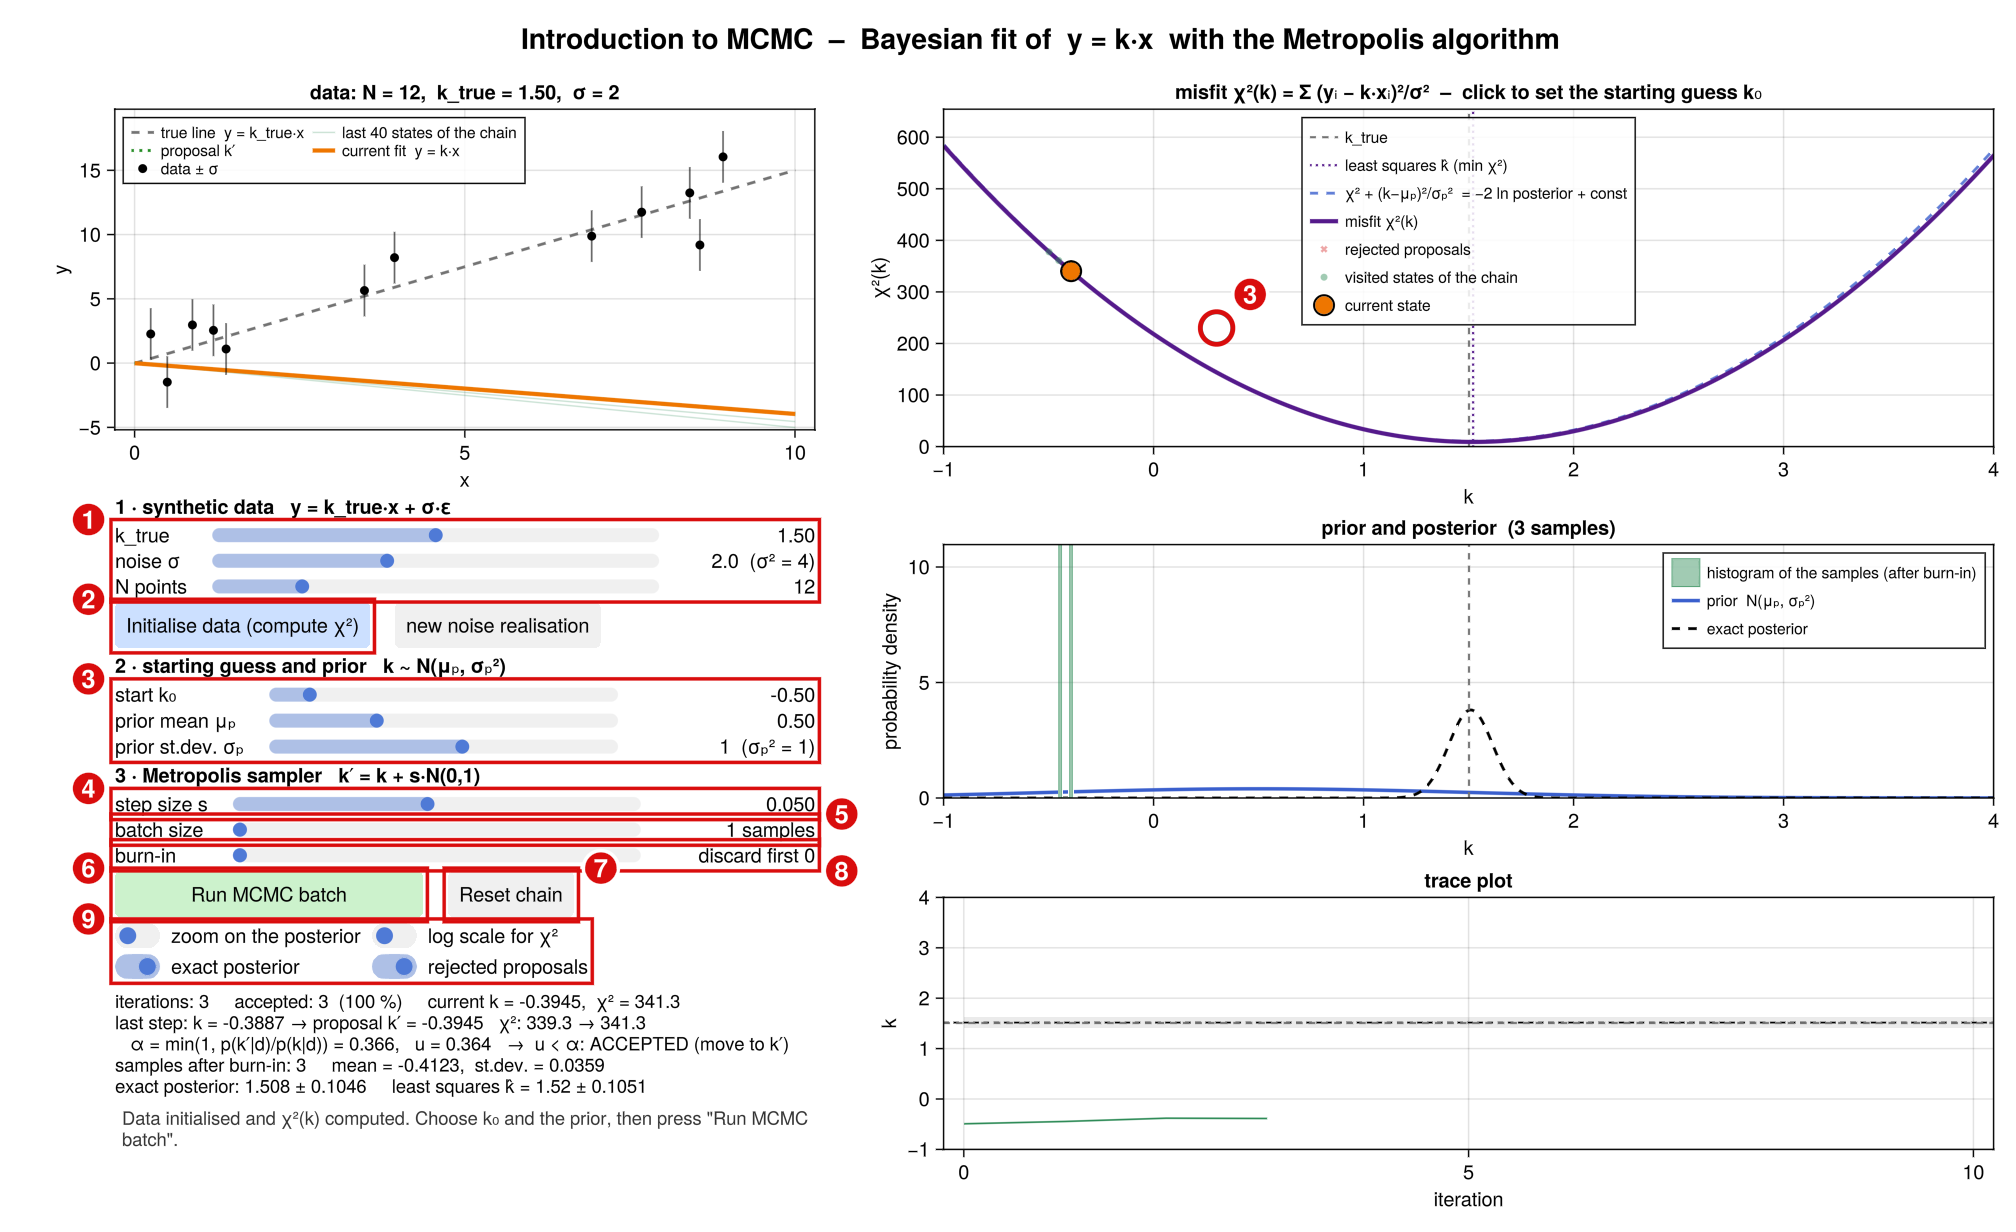
\includegraphics[width=\textwidth]{figures/mcmc1_overview.png}
\caption{Program 1 after three single steps from $k_0=-0.5$ with step size $s=0.05$. The chain sits high on
the left flank of the misfit ($\chi^2\approx340$; the minimum is near $k=1.5$). The info text explains the last
step: the proposal $k'=-0.3945$ was \emph{uphill} ($\chi^2$: $339.3\to341.3$), so
$\alpha=p(k'|d)/p(k|d)=0.366$; the random number $u=0.364$ happened to be smaller, and the step was accepted.}
\label{fig:m1}
\end{figure}

\paragraph{Step by step} (numbers as in Fig.~\ref{fig:m1})
\begin{enumerate}[label=\protect\step{\arabic*}]
\item Choose the data: true slope $k_\text{true}$, noise $\sigma$ (the variance $\sigma^2$ is shown), number of
  points $N$ \dots
\item \dots\ and press \btn{Initialise data (compute $\chi^2$)}: the data are generated and the misfit curve is
  computed. The chain restarts.
\item Choose the starting guess $k_0$ and the prior $\mathcal{N}(\mu_p,\sigma_p^2)$. Changing them restarts
  the chain. A click in the misfit panel also sets $k_0$.
\item \ctl{step size s}: the standard deviation of the random step.
\item \ctl{batch size}: 1, 10, 100 or 1000 iterations per press of the run button.
\item \btn{Run MCMC batch}. With a batch of 1 the proposal is drawn as a dotted line (data panel) and a diamond on
  the misfit curve (green: accepted, red: rejected), and the info text lists $\chi^2$ before and after,
  $\alpha$, $u$ and the decision.
\item \btn{Reset chain}: start again at $k_0$.
\item \ctl{burn-in}: iterations discarded from the histogram and the statistics (grey band in the trace plot).
\item Toggles: zoom on the posterior, logarithmic $\chi^2$ axis, exact posterior, rejected proposals.
\end{enumerate}

\begin{figure}[H]
\centering
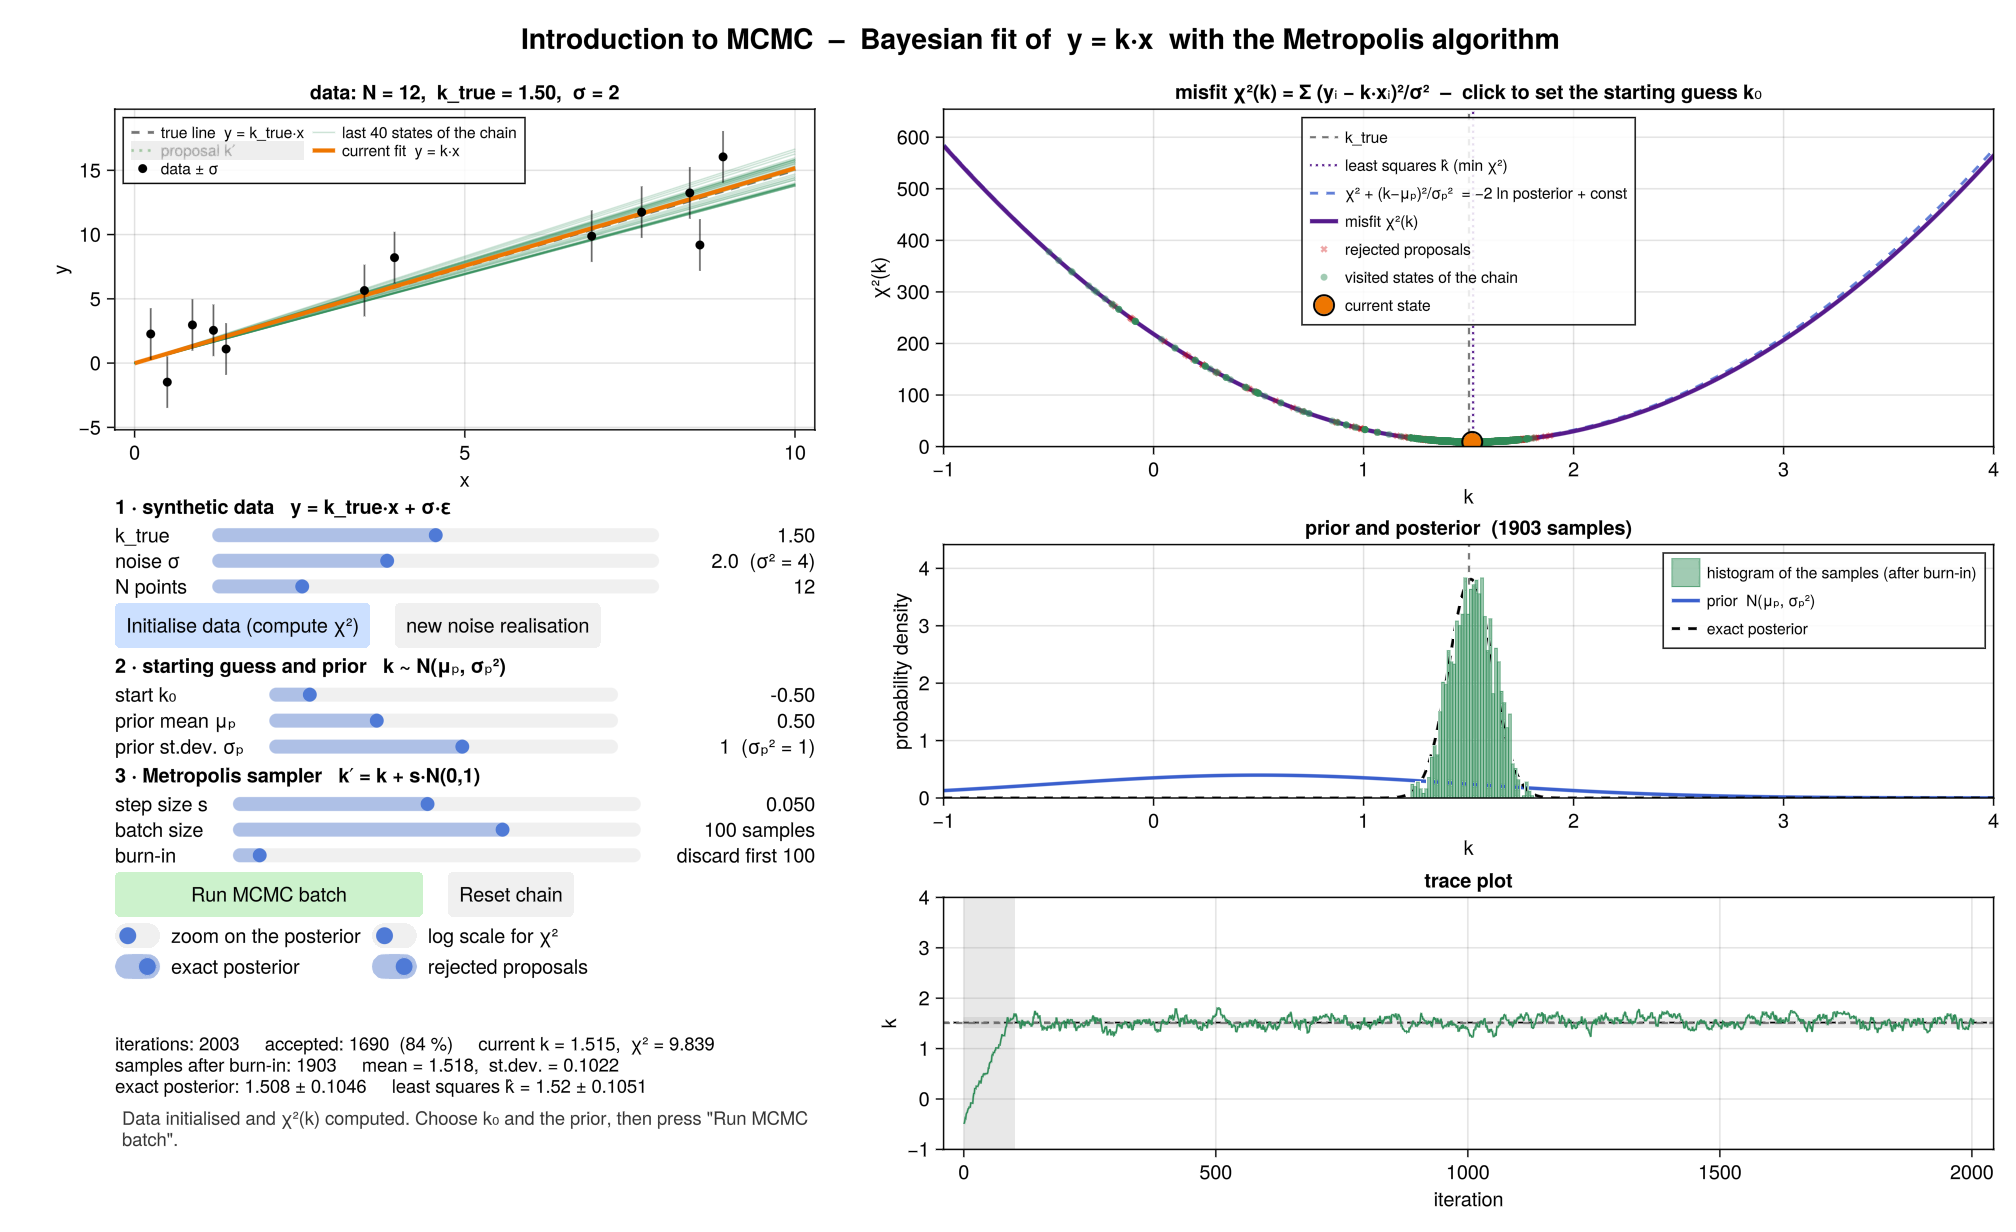
\includegraphics[width=0.49\textwidth]{figures/mcmc1_converged.png}\hfill
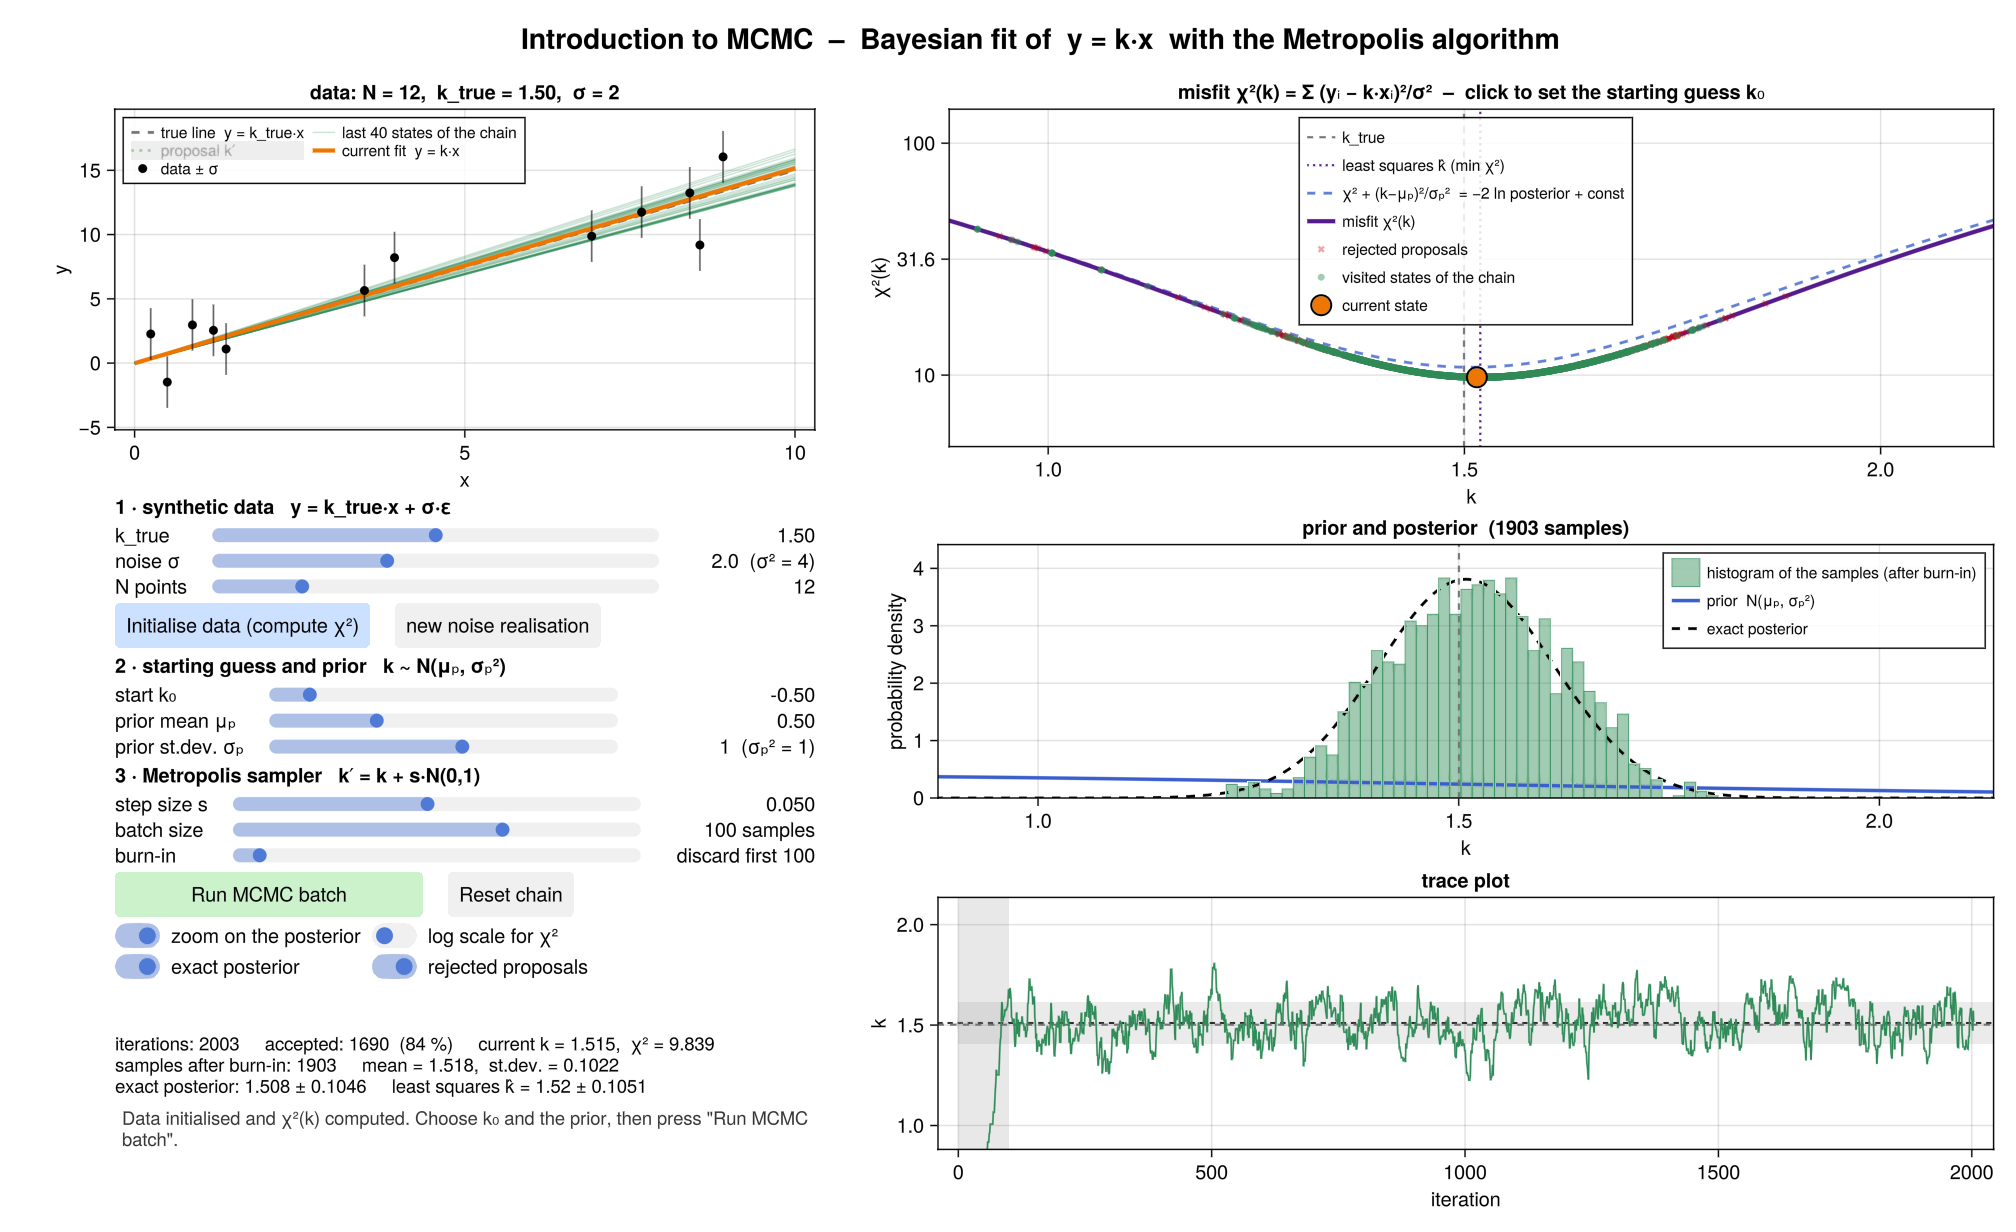
\includegraphics[width=0.49\textwidth]{figures/mcmc1_zoom_log.png}
\caption{Left: 2000 iterations of 100 ($s=0.05$, 84\,\% accepted, burn-in 100). The trace shows the walk down
from $k_0=-0.5$ during the first $\approx 100$ iterations; afterwards the chain fluctuates around the posterior.
Samples: $k=1.518\pm0.102$, exact posterior $1.508\pm0.105$. Right: the same with zoom and logarithmic
$\chi^2$ axis: all visited states lie at the bottom of the misfit valley, within $\Delta\chi^2$ of a few units of
the minimum; the dashed curve $\chi^2+(k-\mu_p)^2/\sigma_p^2$ (the prior added) is almost identical to $\chi^2$,
because the data dominate the weak prior.}
\end{figure}

\begin{figure}[H]
\centering
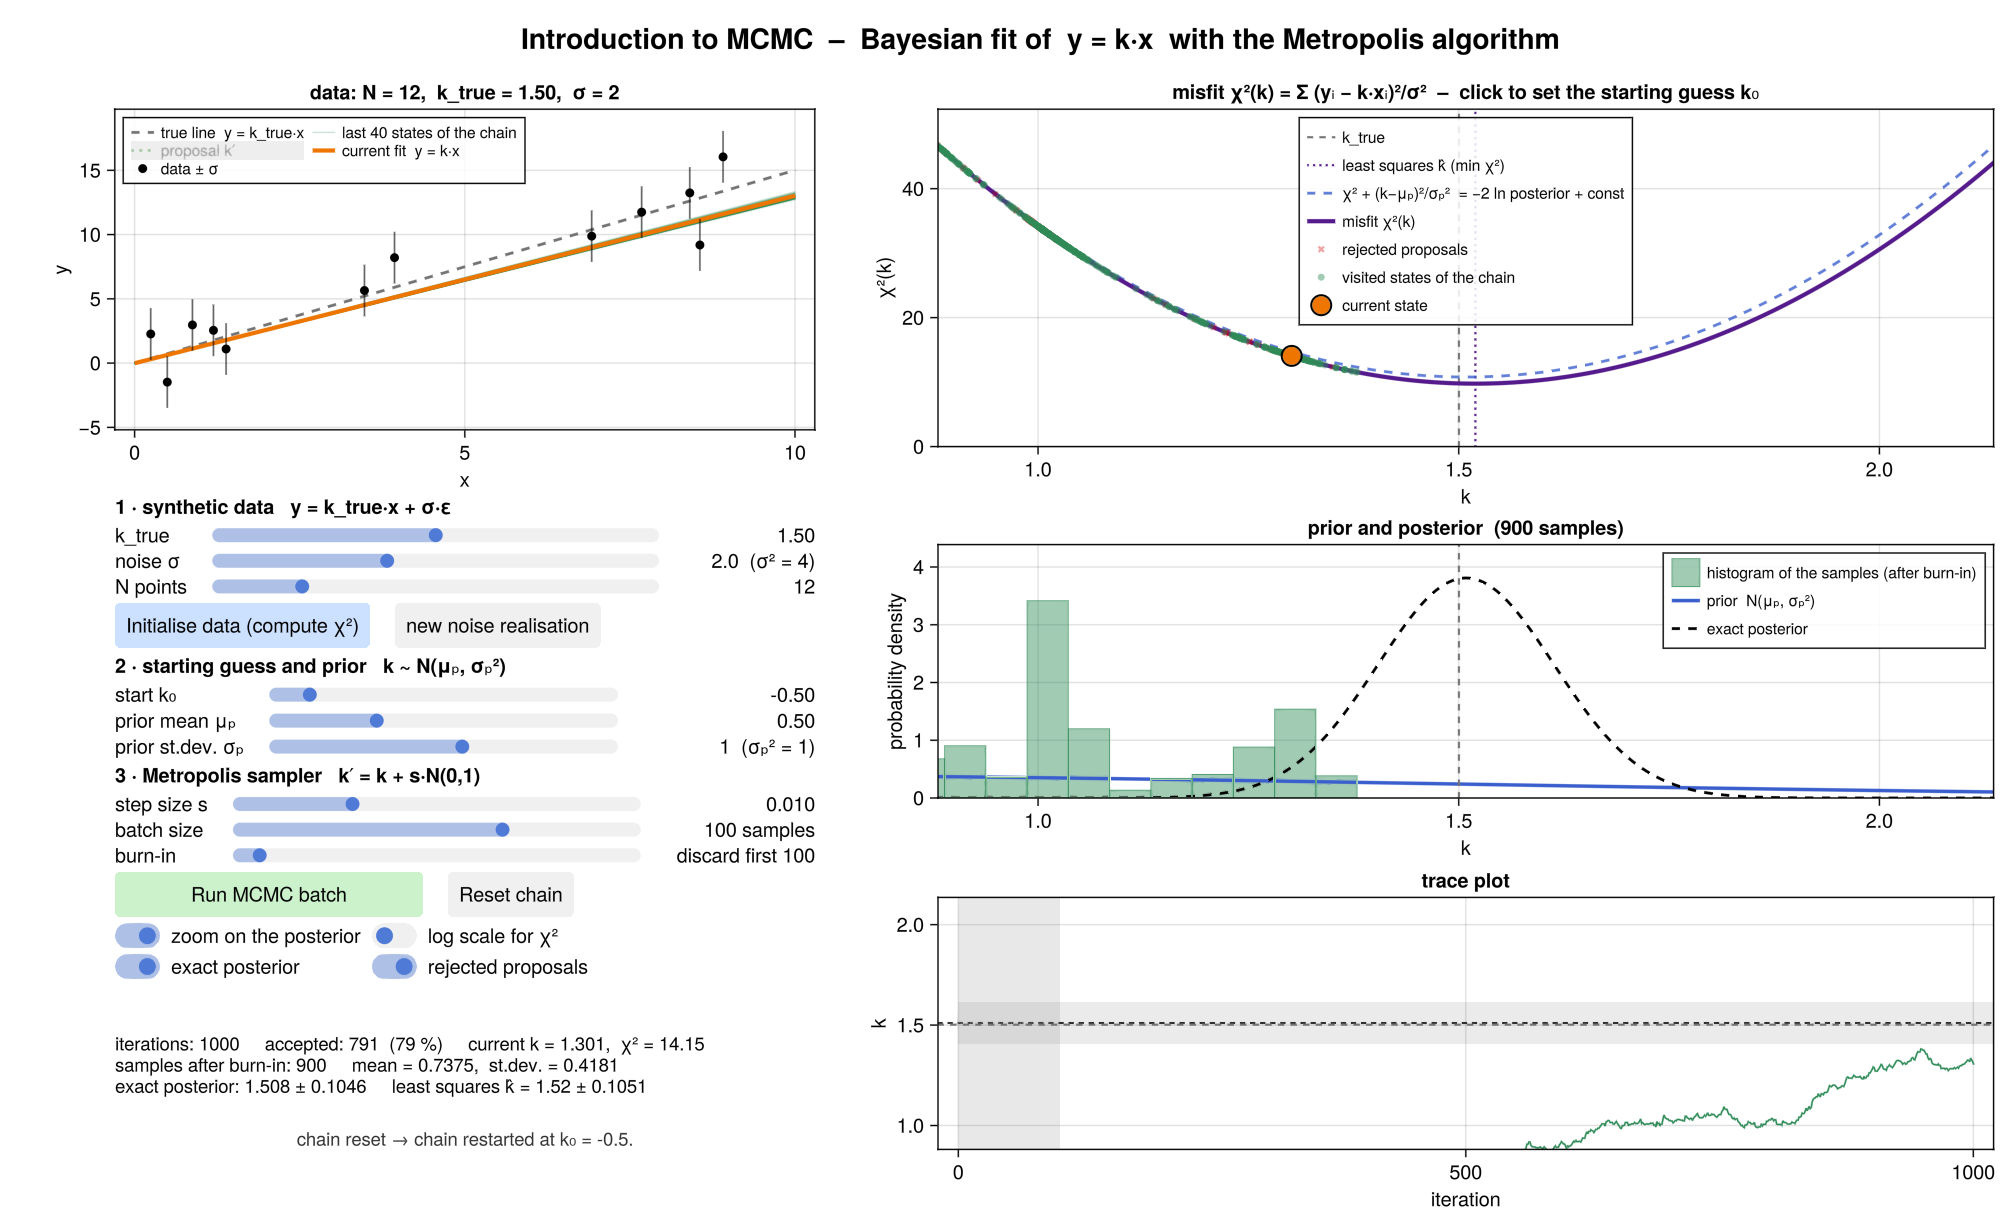
\includegraphics[width=0.329\textwidth]{figures/mcmc1_step_small.png}\hfill
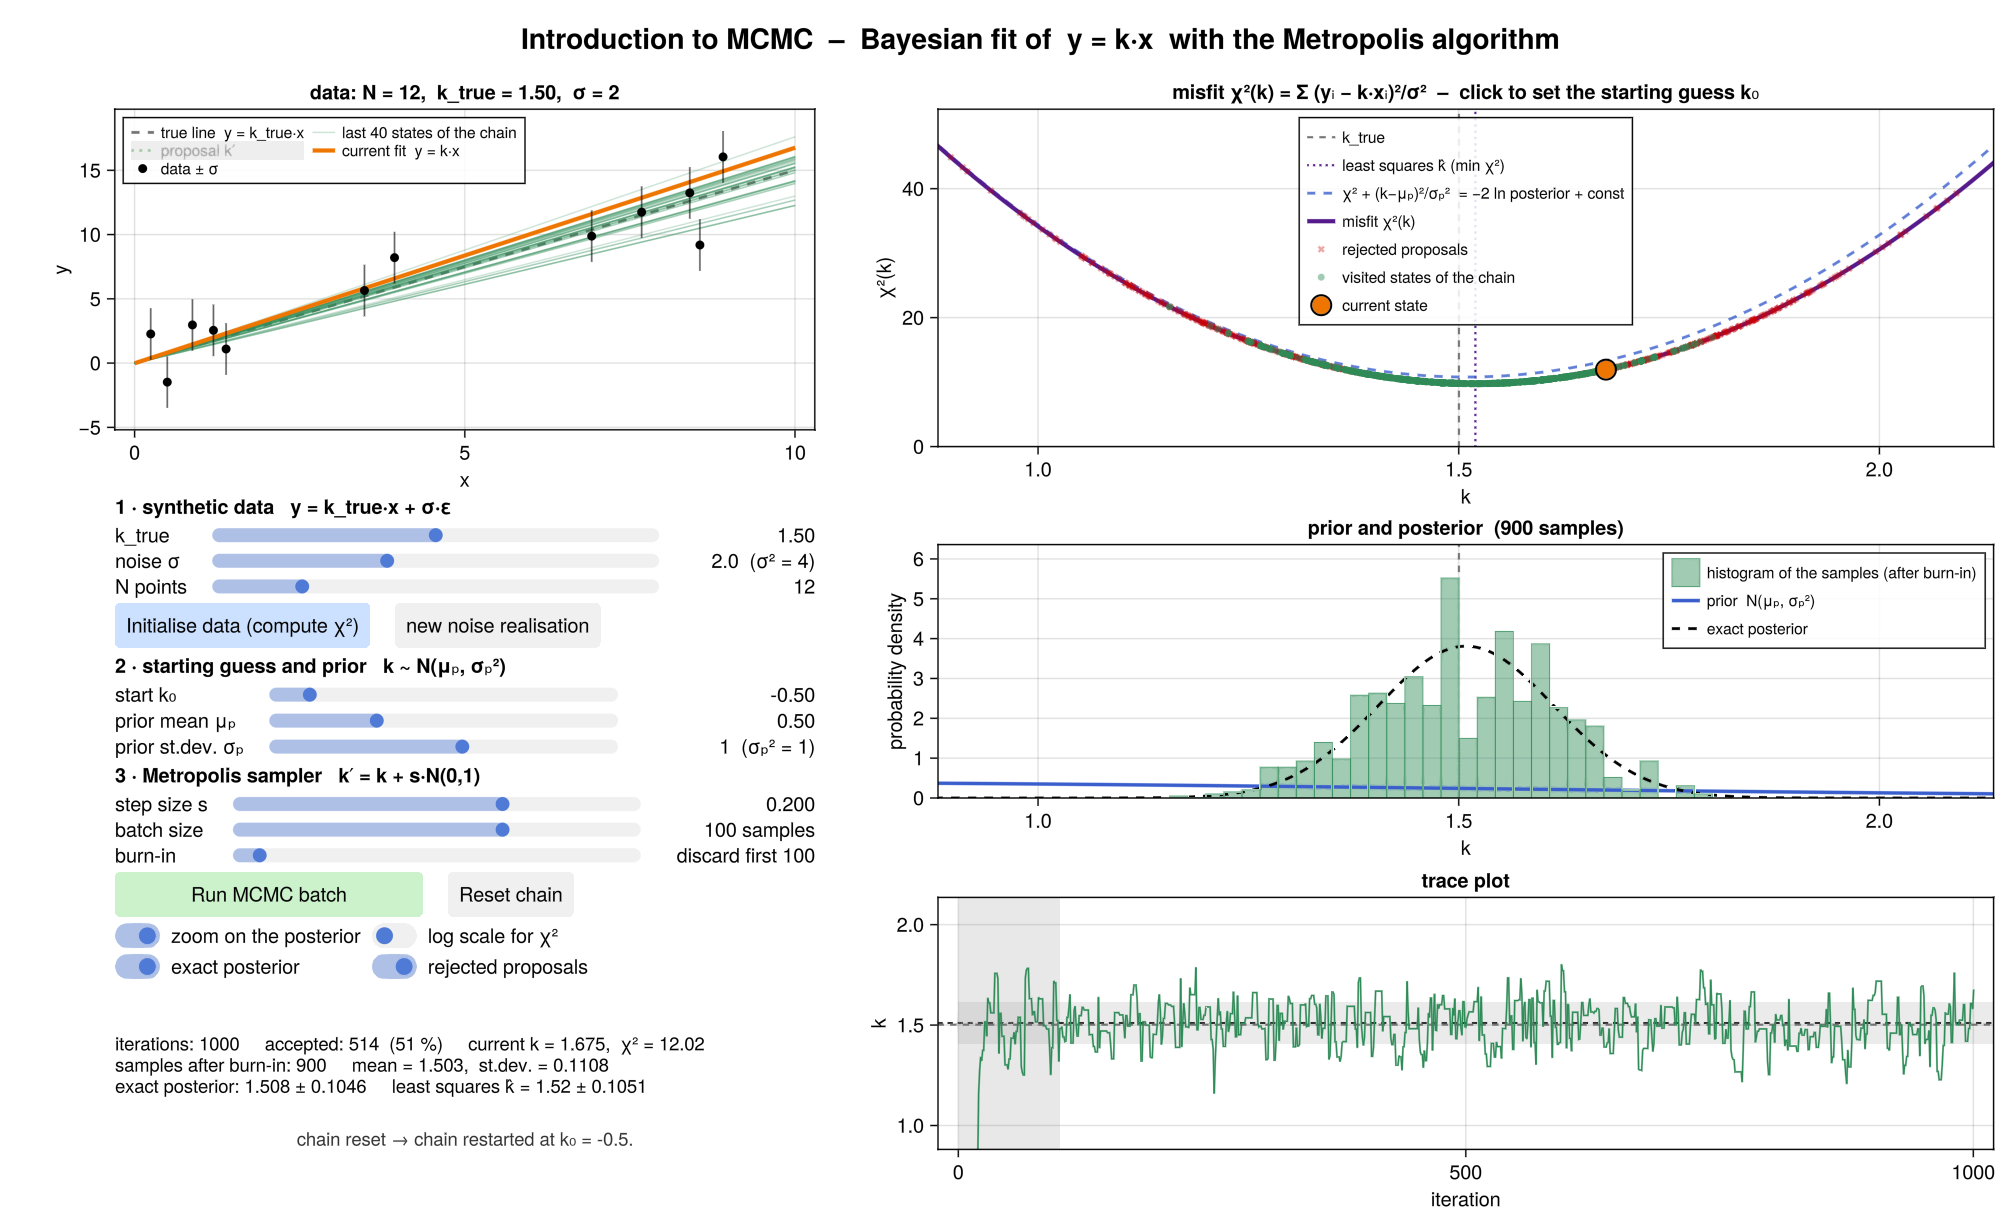
\includegraphics[width=0.329\textwidth]{figures/mcmc1_step_good.png}\hfill
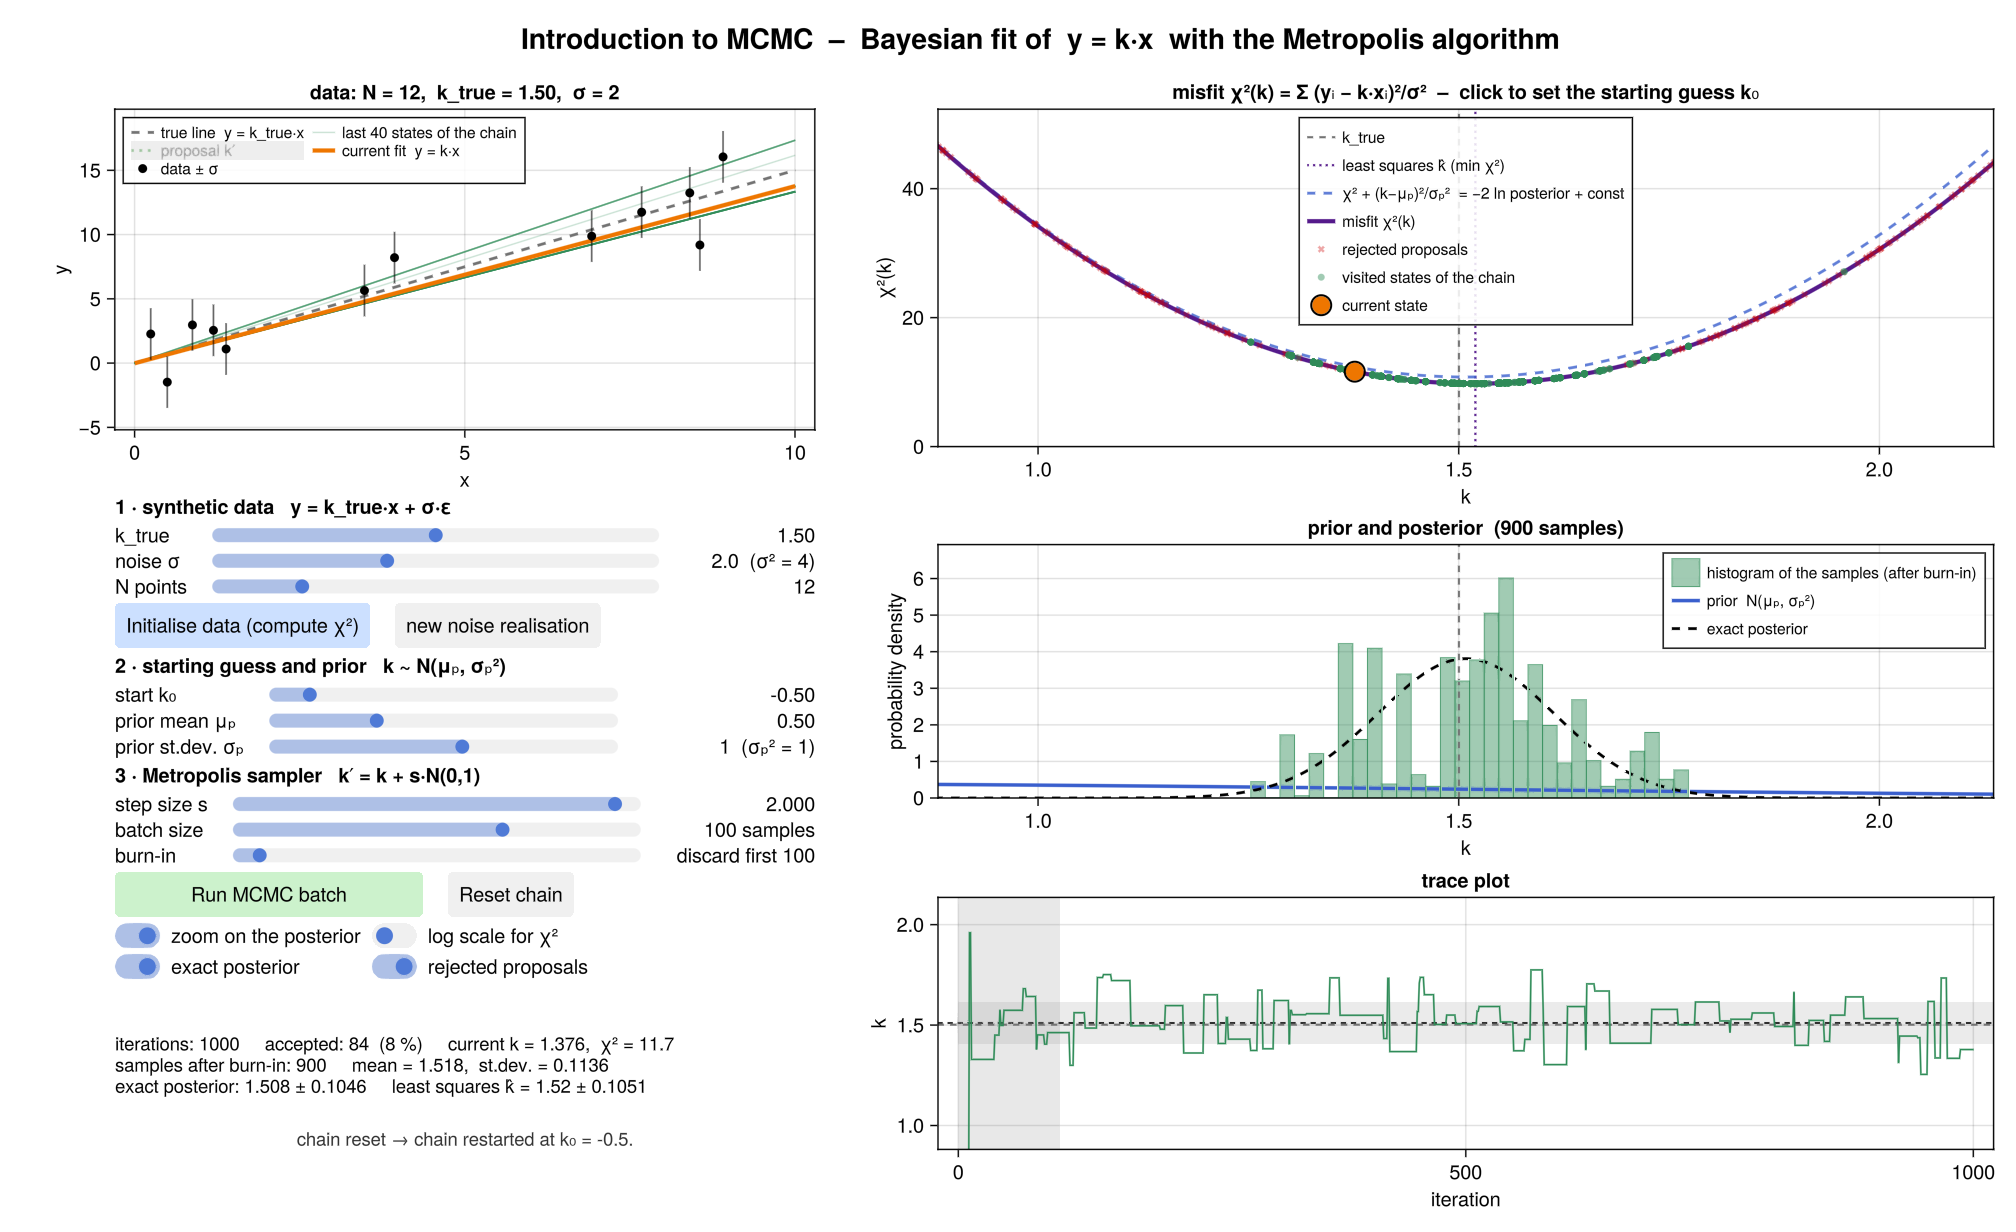
\includegraphics[width=0.329\textwidth]{figures/mcmc1_step_large.png}
\caption{The step size, 1000 iterations from $k_0=-0.5$, burn-in 100. Left, $s=0.01$: 79\,\% accepted, but the
chain has not even reached the posterior (sample mean 0.74). Middle, $s=0.2$: 51\,\% accepted, fast burn-in,
$k=1.503\pm0.111$. Right, $s=2$: only 8\,\% accepted; the chain jumps to the posterior at once but then stands
still for long stretches (flat segments in the trace); $k=1.518\pm0.114$ from only 84 different values.}
\end{figure}

\begin{tryit}
\begin{itemize}
\item Step through the first iterations with a batch of 1 and check $\alpha=e^{-\Delta\chi^2/2}$ (times the
  prior ratio) for uphill steps. How often is a step with $\Delta\chi^2=4$ accepted?
\item Find the step size that gives an acceptance of about 45\,\% and compare the trace with
  $s=0.01$ and $s=2$.
\item Increase the noise $\sigma$ or decrease $N$: the posterior becomes wider and the prior more important.
  Move the prior mean $\mu_p$ and watch the exact posterior move. With $N=3$, $\sigma=5$ and a narrow prior
  ($\sigma_p=0.2$), where does the posterior lie?
\item Click in the misfit panel far from the minimum (e.g.\ $k=3.5$) and run: how long is the burn-in?
\end{itemize}
\end{tryit}

%==============================================================================
\clearpage
\section{Program 2 – Metropolis--Hastings and the Hastings correction}\label{sec:m2}
%==============================================================================
\textbf{File:} \file{Introduction\_MCMC\_2.jl}.\quad Same problem as Program~1, but the proposal can be
asymmetric and the acceptance is \eqref{eq:mh}. Four Gaussian proposals $k'\sim\mathcal{N}(c(k),s^2)$ are
available:
\begin{center}\small
\begin{tabular}{@{}lll@{}}
\toprule
proposal & centre $c(k)$ & Hastings ratio \\
\midrule
1 symmetric random walk & $k$ & $=1$ (Program 1) \\
2 random walk with drift & $k+d$ & $\ne1$: favours steps in the direction of $d$ \\
3 independence sampler & $m_q$ (independent of $k$) & $\ne1$ \\
4 Langevin (MALA) & $k+\tfrac12 s^2\,\partial_k\ln p(k|d)$ & $\ne1$: pushed uphill by the gradient \\
\bottomrule
\end{tabular}
\end{center}

\begin{figure}[H]
\centering
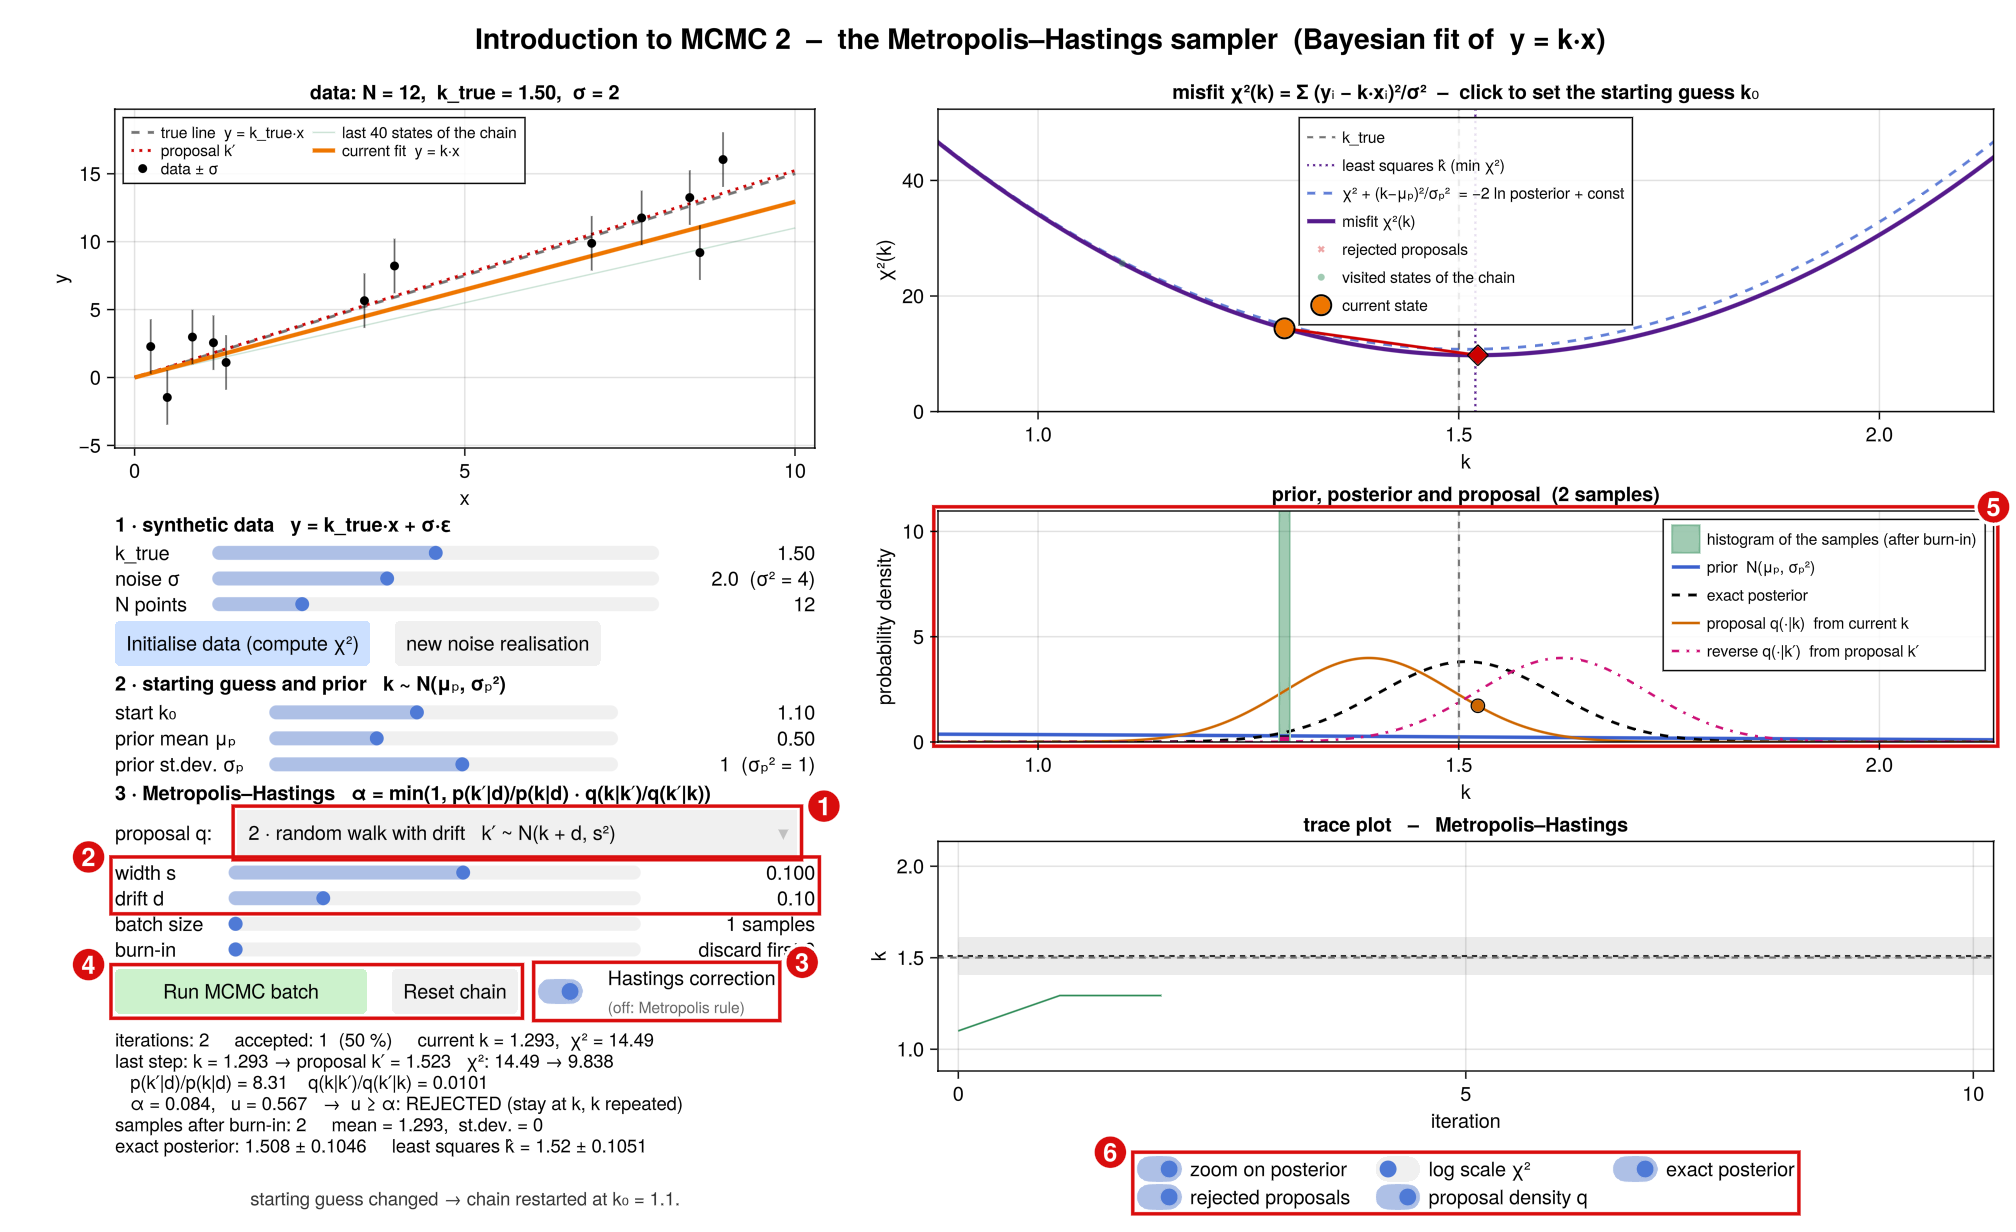
\includegraphics[width=\textwidth]{figures/mcmc2_overview.png}
\caption{Program 2 with the drift proposal ($s=0.1$, $d=0.1$), zoomed, after two single steps from $k_0=1.1$.
The posterior panel shows the forward proposal density $q(\cdot|k)$ (orange, centred at $k+d$) and the reverse
density $q(\cdot|k')$ (pink). The last step went \emph{downhill} ($\chi^2$: $14.49\to9.84$, posterior ratio
8.31), yet it was rejected: moving forward is easy for this proposal ($q(k'|k)$ large), moving back is hard
($q(k|k')$ small), and the Hastings ratio $0.0101$ gives $\alpha=0.084$.}
\label{fig:m2}
\end{figure}

\paragraph{Step by step} (numbers as in Fig.~\ref{fig:m2}; data and prior as in Program~1)
\begin{enumerate}[label=\protect\step{\arabic*}]
\item Choose the proposal. The chain is not restarted (the target is unchanged).
\item \ctl{width s} and, for proposals 2 and 3, the drift $d$ or the centre $m_q$ (the label of the second
  slider changes with the proposal).
\item \ctl{Hastings correction}: off, the plain Metropolis rule \eqref{eq:alpha} is used. The trace title turns
  red as a warning.
\item \btn{Run MCMC batch} and \btn{Reset chain}. With a batch of 1 the info text lists the posterior ratio,
  the Hastings ratio, $\alpha$ and $u$.
\item The posterior panel with the proposal densities: after a single step the forward density $q(\cdot|k)$ with
  $q(k'|k)$ marked, and the reverse density $q(\cdot|k')$ with $q(k|k')$ marked. Their ratio is the Hastings
  ratio.
\item Toggles, including \ctl{proposal density q}.
\end{enumerate}

\begin{figure}[H]
\centering
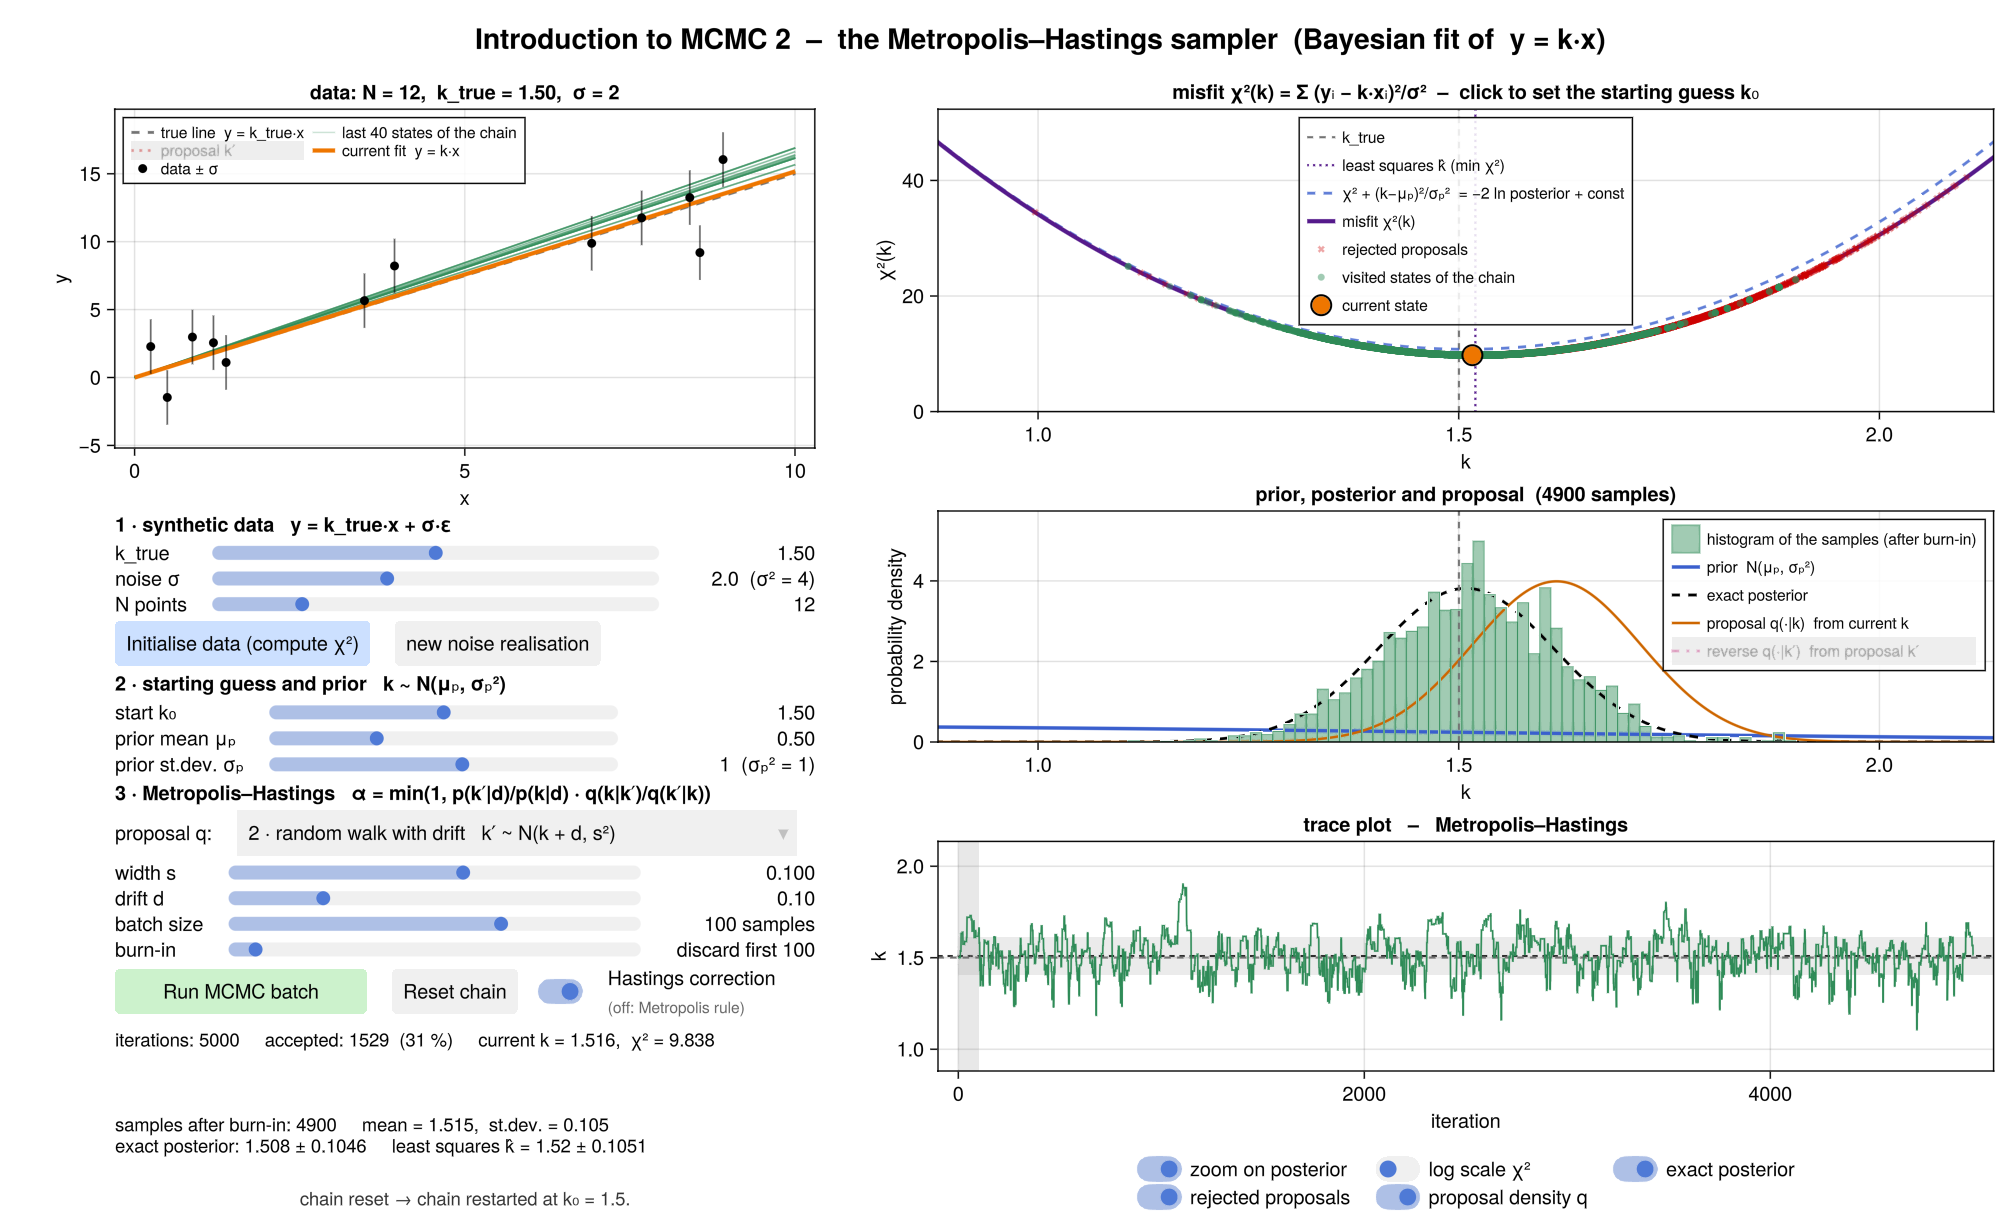
\includegraphics[width=0.49\textwidth]{figures/mcmc2_drift_on.png}\hfill
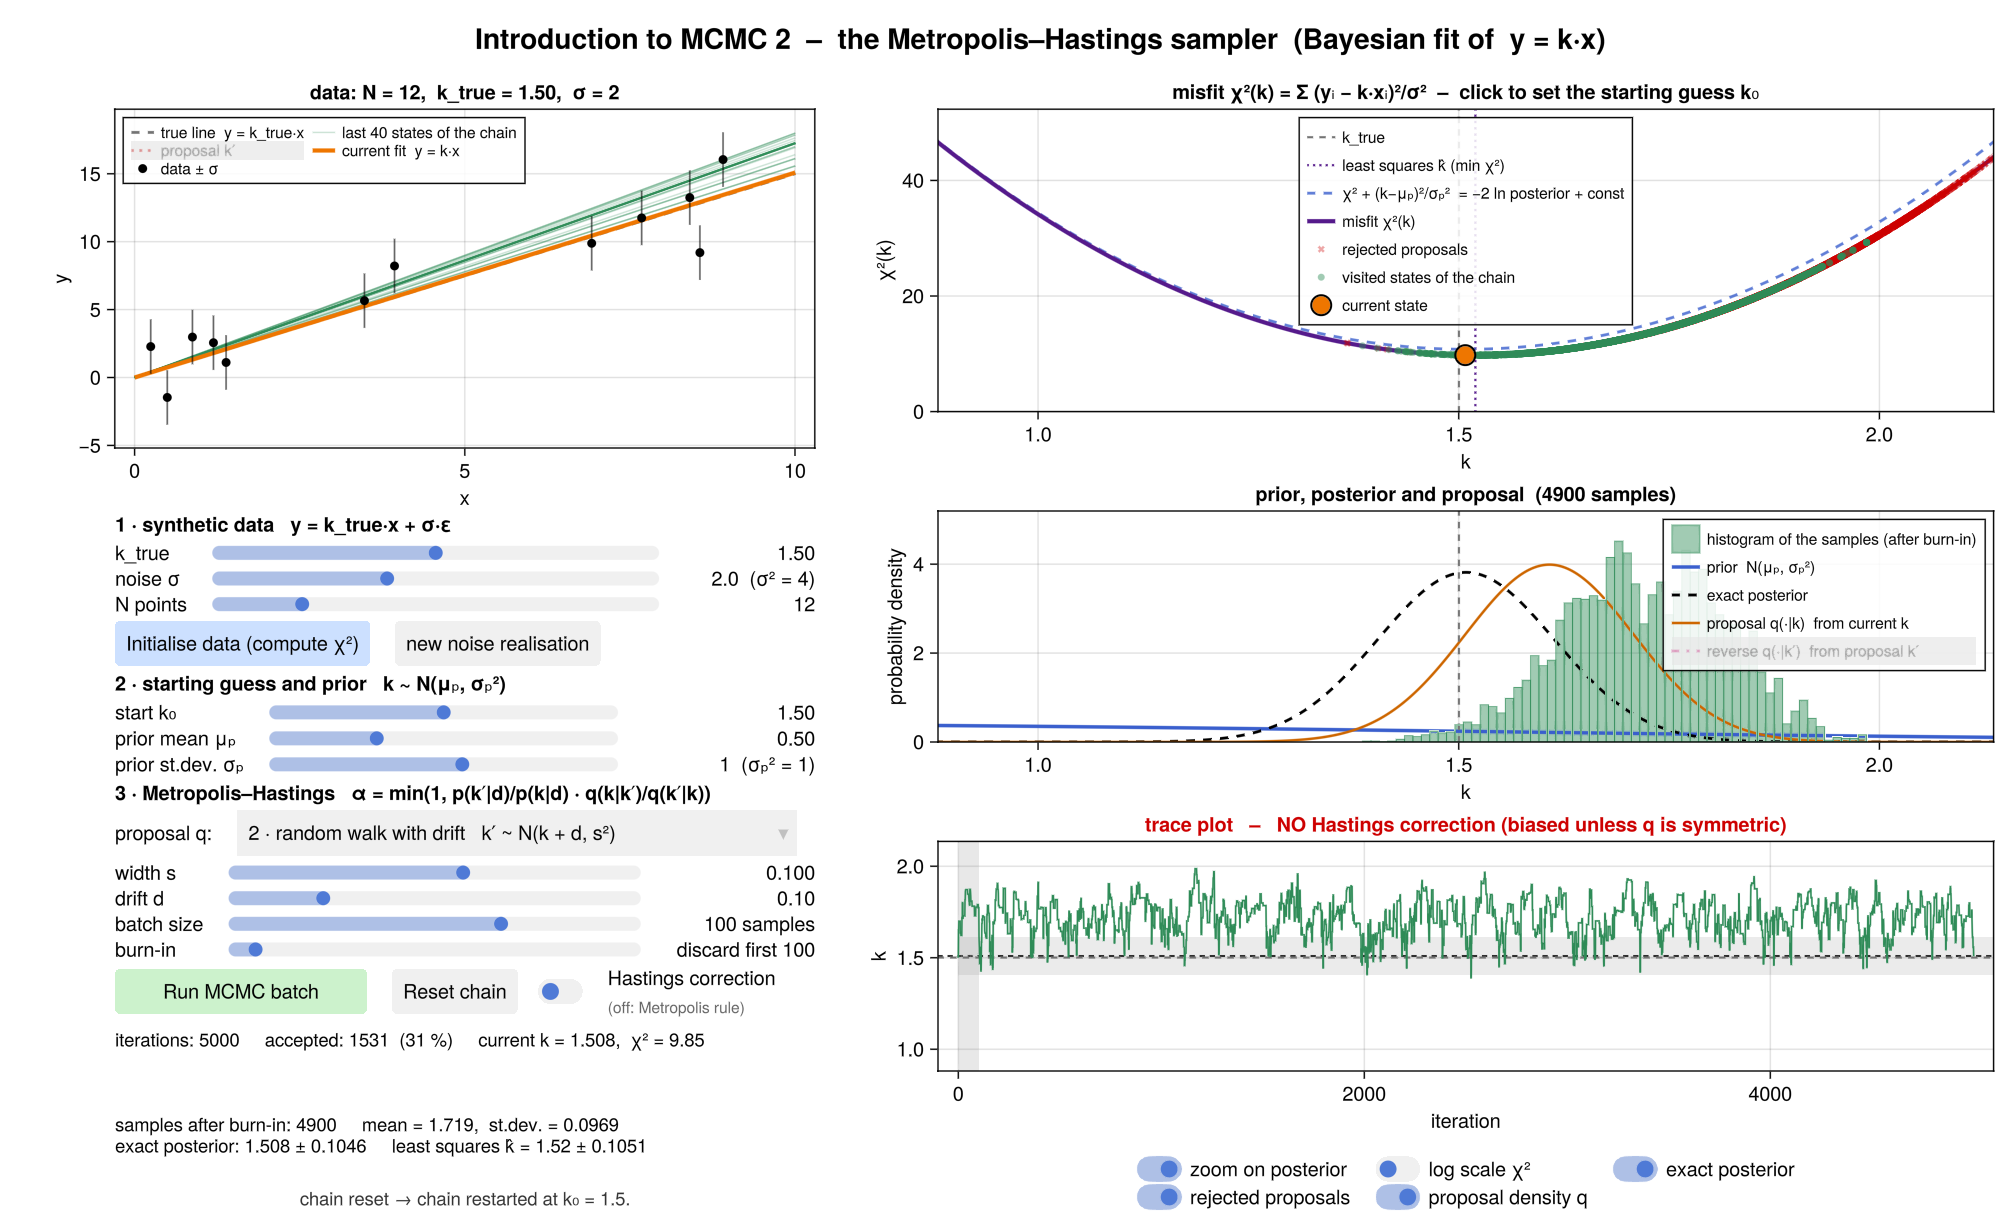
\includegraphics[width=0.49\textwidth]{figures/mcmc2_drift_off.png}
\caption{The drift proposal, 5000 iterations, burn-in 100. Left, with the Hastings correction:
$k=1.515\pm0.105$, the exact posterior is $1.508\pm0.105$. Right, without: $k=1.719\pm0.097$, the histogram is
shifted by two posterior standard deviations in the direction of the drift. Both chains look perfectly well
behaved in the trace plot; only the comparison with the exact posterior reveals the error.}
\end{figure}

\begin{figure}[H]
\centering
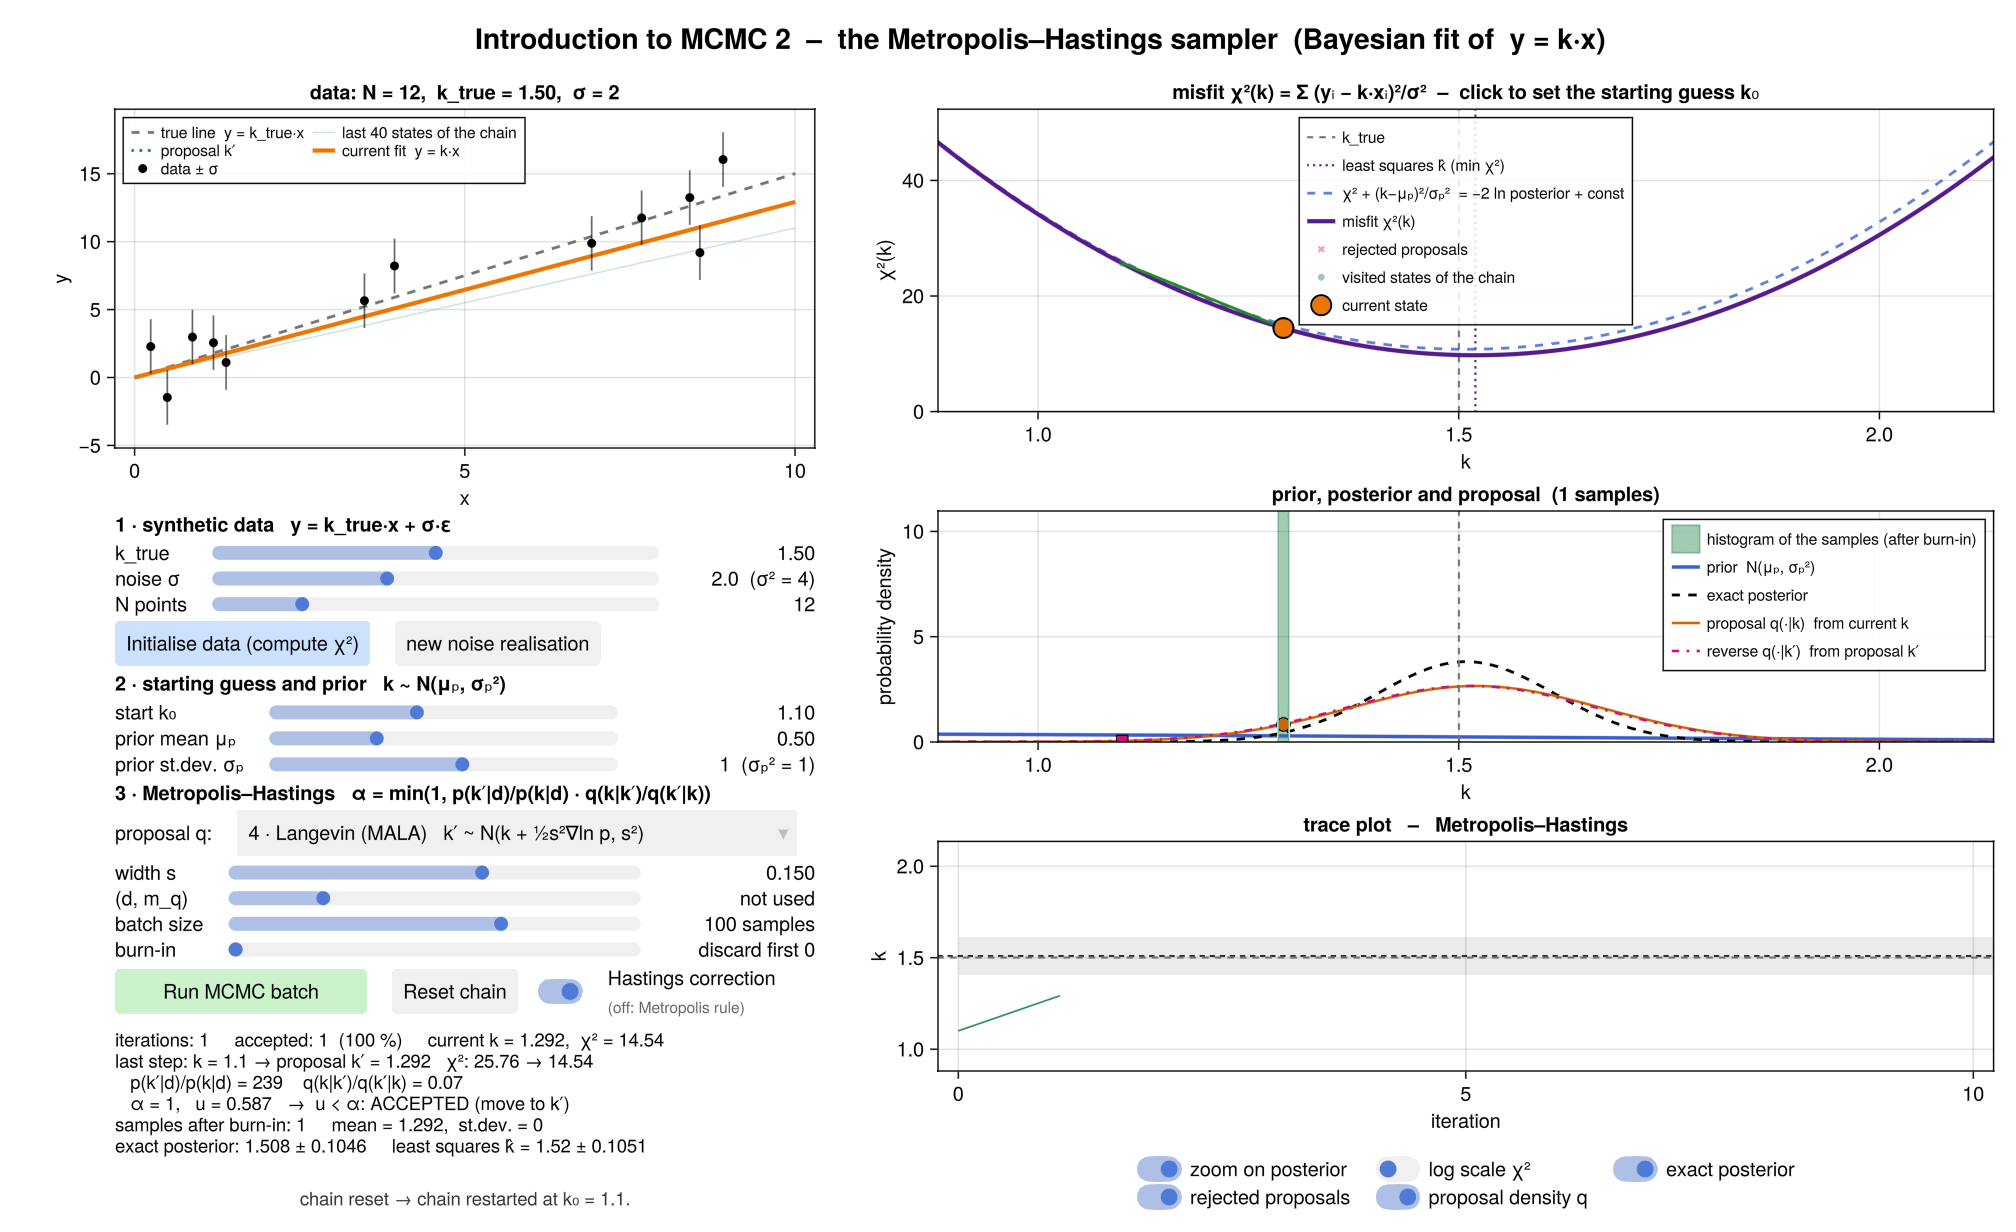
\includegraphics[width=0.49\textwidth]{figures/mcmc2_mala_step.png}\hfill
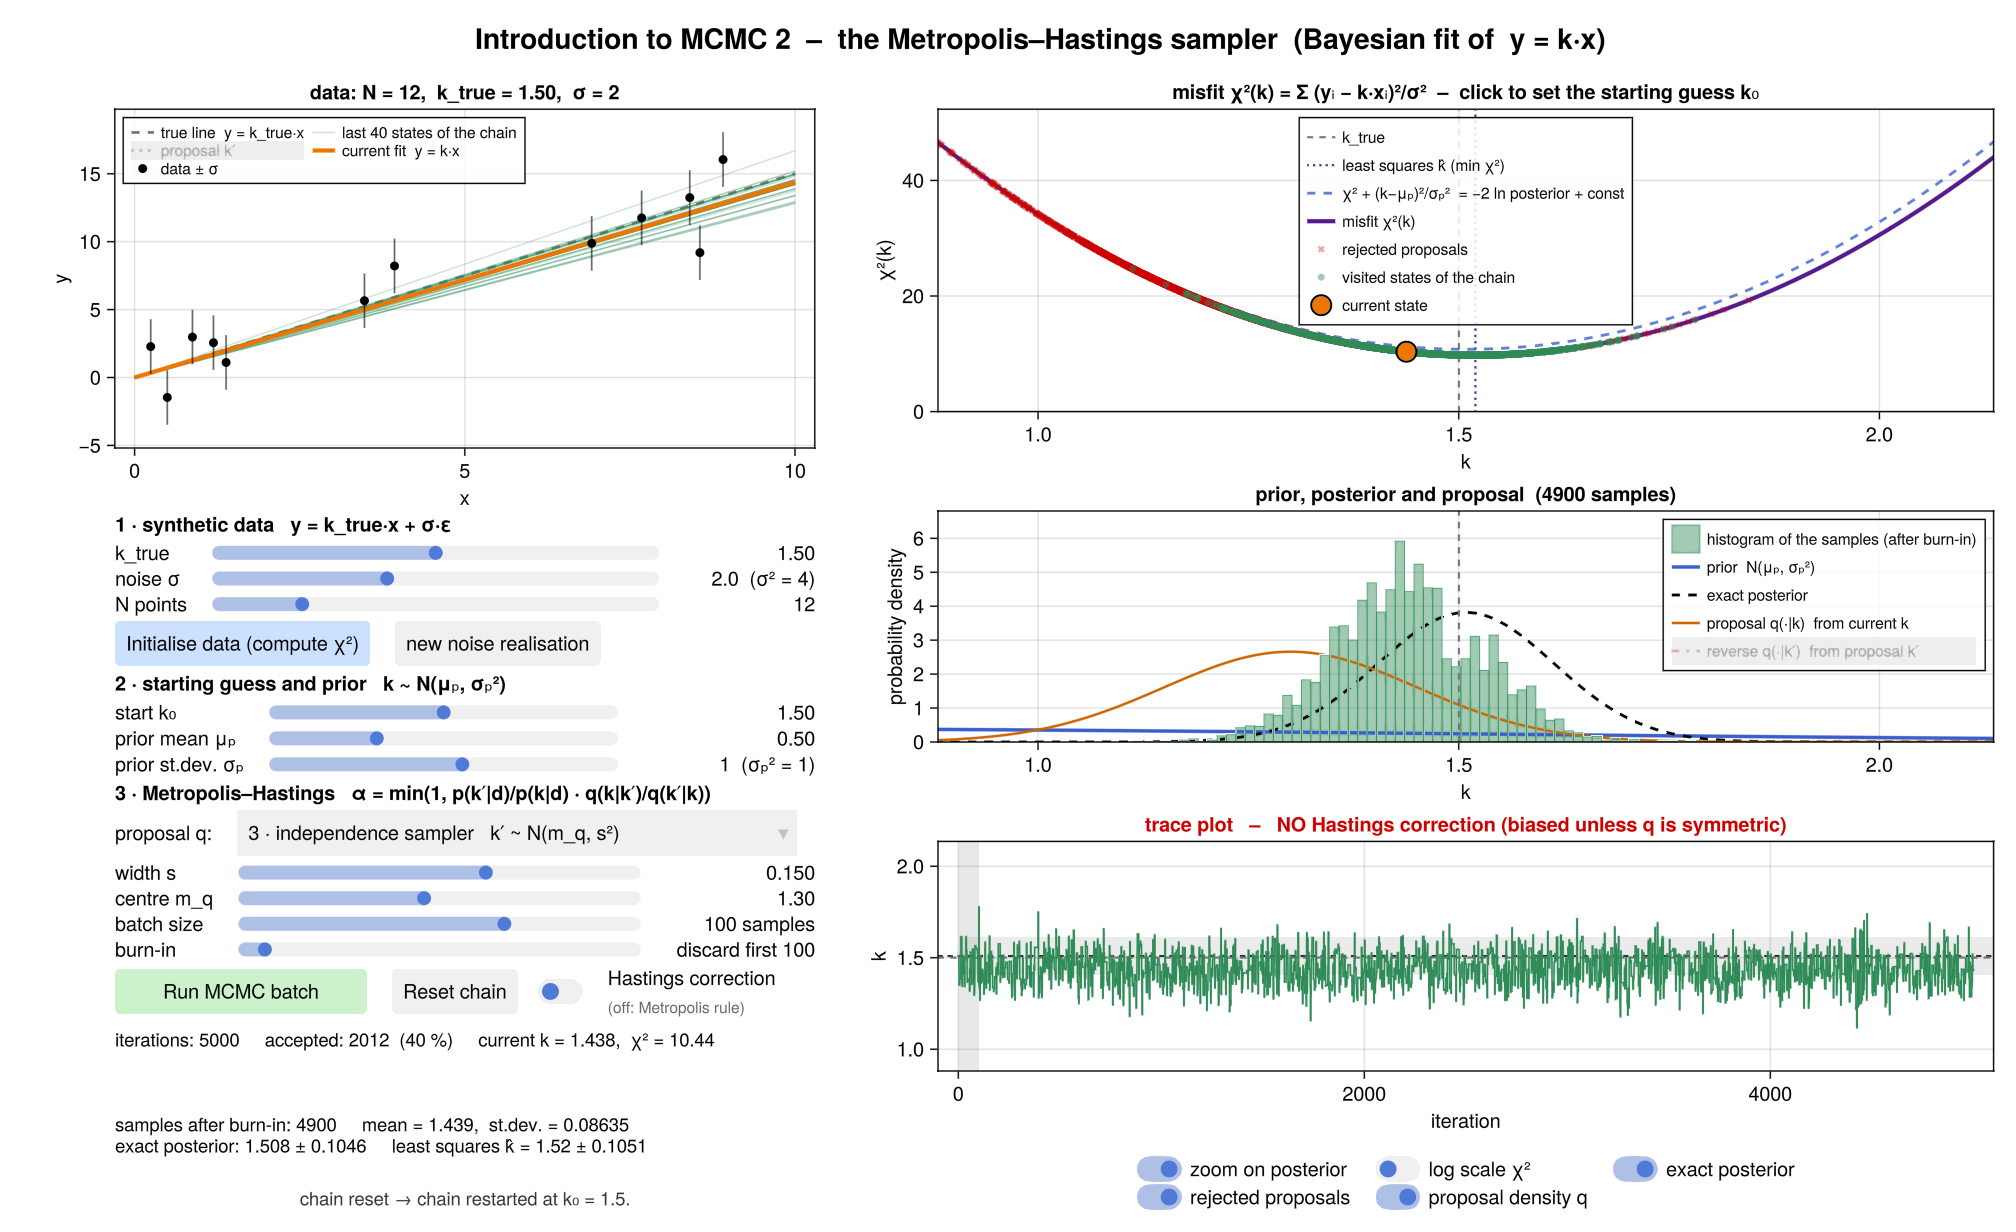
\includegraphics[width=0.49\textwidth]{figures/mcmc2_indep_off.png}
\caption{Left: one Langevin (MALA) step from $k=1.1$, $s=0.15$. The gradient pushes the proposal uphill: the
forward density $q(\cdot|k)$ is centred near the posterior, and $k'=1.292$ is accepted (posterior ratio 239,
Hastings ratio 0.07, $\alpha=1$). Right: independence sampler $\mathcal{N}(1.3,0.15^2)$ \emph{without} the
Hastings correction, 5000 iterations: $k=1.439\pm0.086$. The chain samples the product $p(k|d)\,q(k)$ (which has
mean 1.440 and standard deviation 0.086), not the posterior.}
\end{figure}

\begin{tryit}
\begin{itemize}
\item With the drift proposal, switch the Hastings correction off and on, pressing \btn{Reset chain} each
  time. Change the sign of the drift: in which direction is the histogram shifted now?
\item Symmetric random walk (proposal 1): does the Hastings toggle make any difference? Why?
\item Independence sampler with $m_q$ close to the posterior mean and $s\approx0.15$: almost every proposal is
  accepted, the samples are nearly independent. Move $m_q$ to 0.5 and $s$ to 0.05: what happens to the
  acceptance and the trace?
\item MALA: start far away ($k_0=-0.5$) and compare the burn-in with Program~1. Then make $s$ large (0.3): what
  happens without the Hastings correction?
\end{itemize}
\end{tryit}

%==============================================================================
\clearpage
\section{Program 3 – Metropolis--Hastings for two parameters}\label{sec:m3}
%==============================================================================
\textbf{File:} \file{Introduction\_MCMC\_3.jl}.\quad Fit of $y=a+k\,x$. The upper right is a \emph{corner
plot}: the misfit map $\chi^2(k,a)$ with the chain, the marginal posterior of $k$ above it and that of $a$ to its
right. With $x$ between 0 and 10 the two parameters are strongly anti-correlated: a steeper line through the
data needs a lower intercept, so the posterior is a narrow, tilted ellipse (correlation $\rho=-0.77$ for the
default data). This is the new difficulty in more than one dimension. Five proposals $\vth'\sim\mathcal{N}(c,s^2C)$:
isotropic random walk ($C=I$), one parameter at a time, random walk with a learned covariance ($C=\hat\Sigma$),
independence sampler ($c=$ learned mean, $C=\hat\Sigma$) and Langevin (MALA).

\begin{figure}[H]
\centering
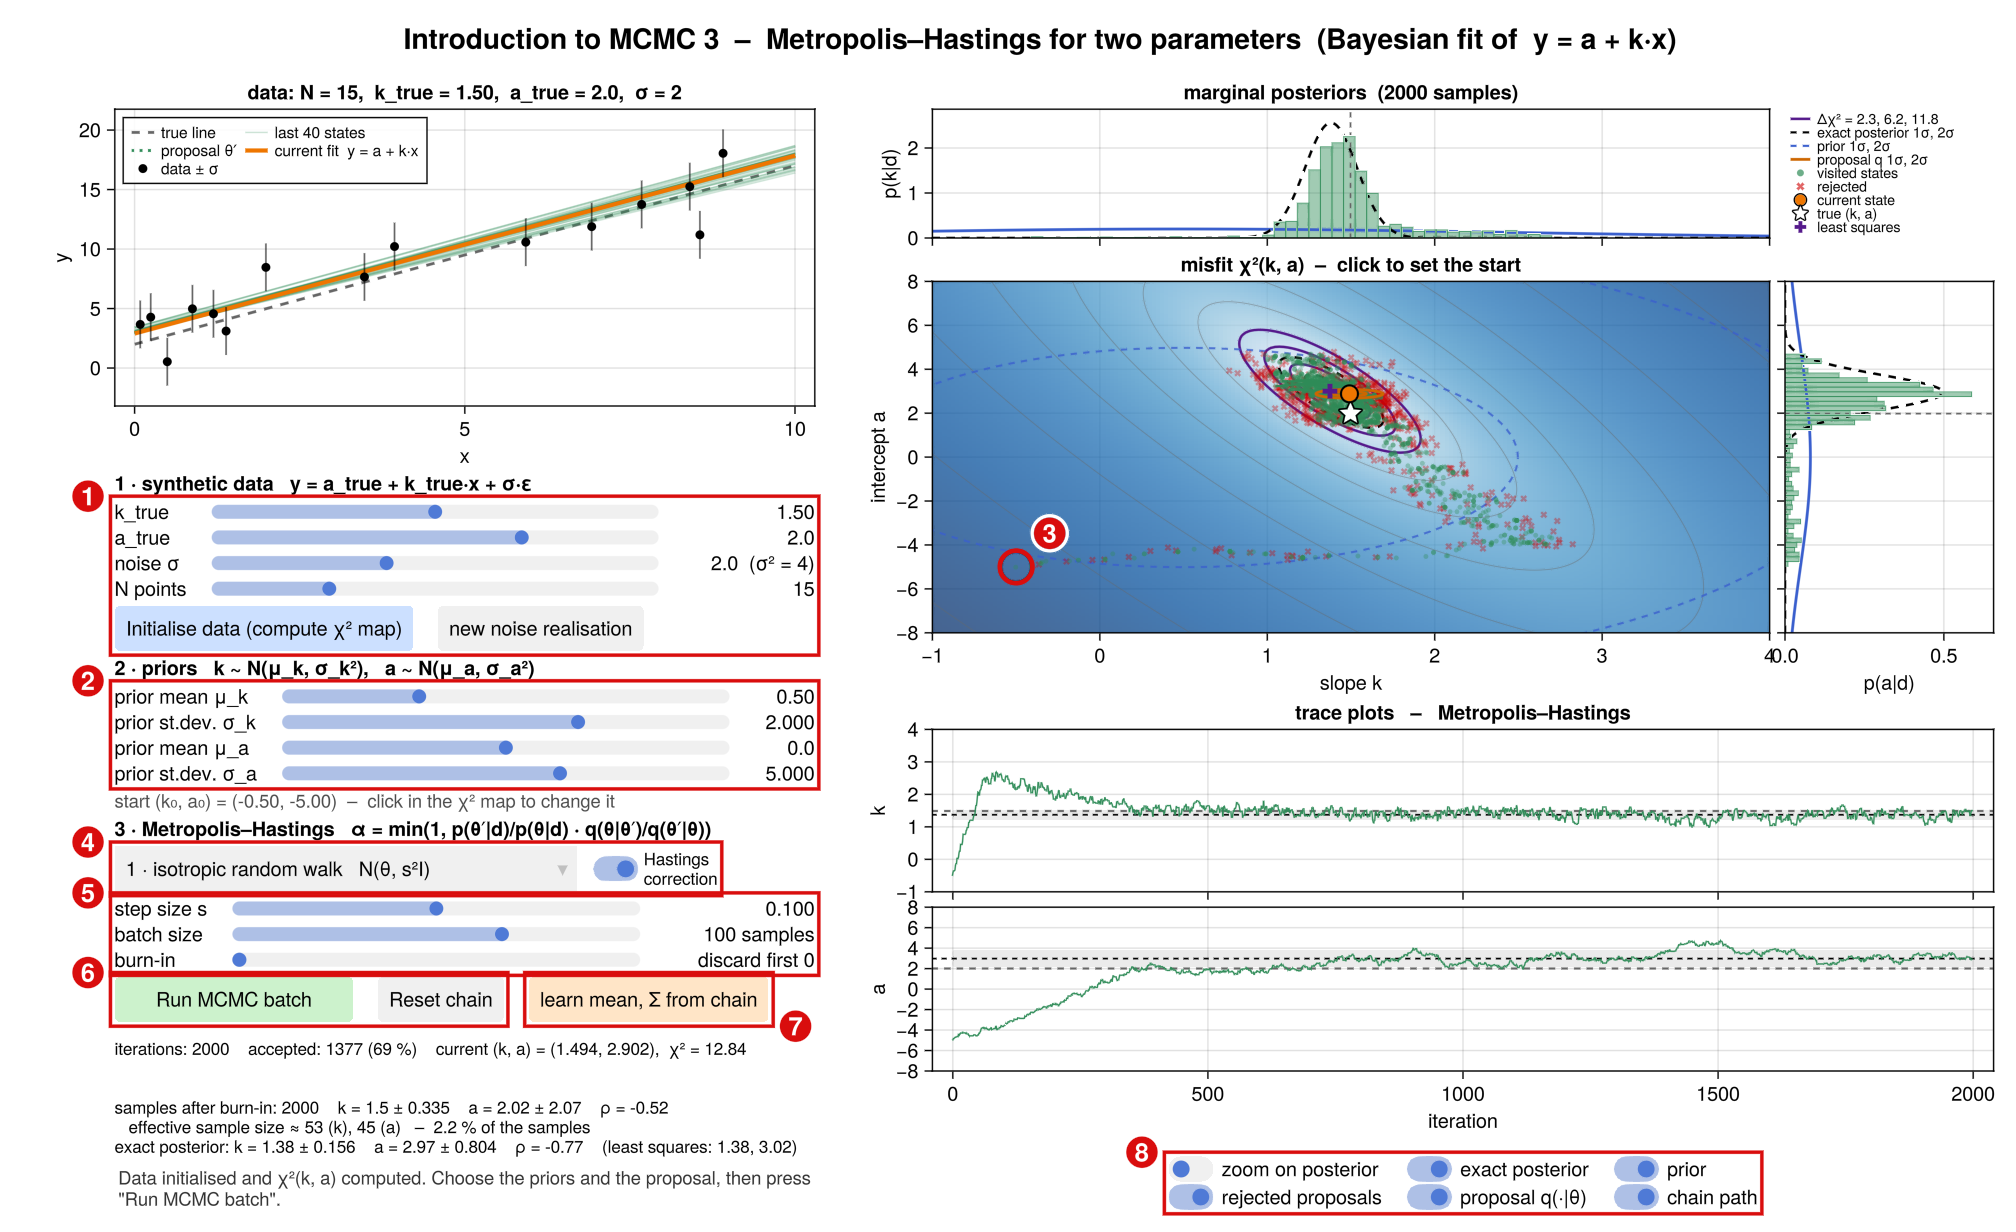
\includegraphics[width=\textwidth]{figures/mcmc3_overview.png}
\caption{Program 3 after 2000 iterations of the isotropic random walk ($s=0.1$) from $(k_0,a_0)=(-0.5,-5)$.
The chain first slides down the steep side of the valley, then creeps along its axis; the trace of $a$ shows the
slow drift for the first $\approx500$ iterations. Effective sample size: only 53 ($k$) and 45 ($a$), 2.2\,\%
of the samples; the statistics (burn-in not removed) are still far from the exact values
$k=1.38\pm0.156$, $a=2.97\pm0.804$, $\rho=-0.77$.}
\label{fig:m3}
\end{figure}

\paragraph{Step by step} (numbers as in Fig.~\ref{fig:m3})
\begin{enumerate}[label=\protect\step{\arabic*}]
\item Data: true slope and intercept, noise, number of points; \btn{Initialise data (compute $\chi^2$ map)}.
\item Independent Gaussian priors for $k$ and $a$ (blue dashed ellipses: 1$\sigma$ and 2$\sigma$).
\item Click in the map to set the starting point; the chain restarts.
\item Proposal menu and \ctl{Hastings correction} (needed for proposals 4 and 5).
\item \ctl{step size s}, \ctl{batch size}, \ctl{burn-in}.
\item \btn{Run MCMC batch}, \btn{Reset chain}.
\item \btn{learn mean, $\Sigma$ from chain}: the mean and covariance of the samples after burn-in are stored and used by
  proposals 3 and 4 (two-stage adaptive MCMC: learn during a pilot run, then keep $\hat\Sigma$ fixed). The
  proposal density $q(\cdot|\vth)$ is drawn as orange ellipses at the current state.
\item Toggles: zoom, exact posterior (black dashed ellipses and marginals), prior, rejected proposals, proposal,
  chain path.
\end{enumerate}

\begin{figure}[H]
\centering
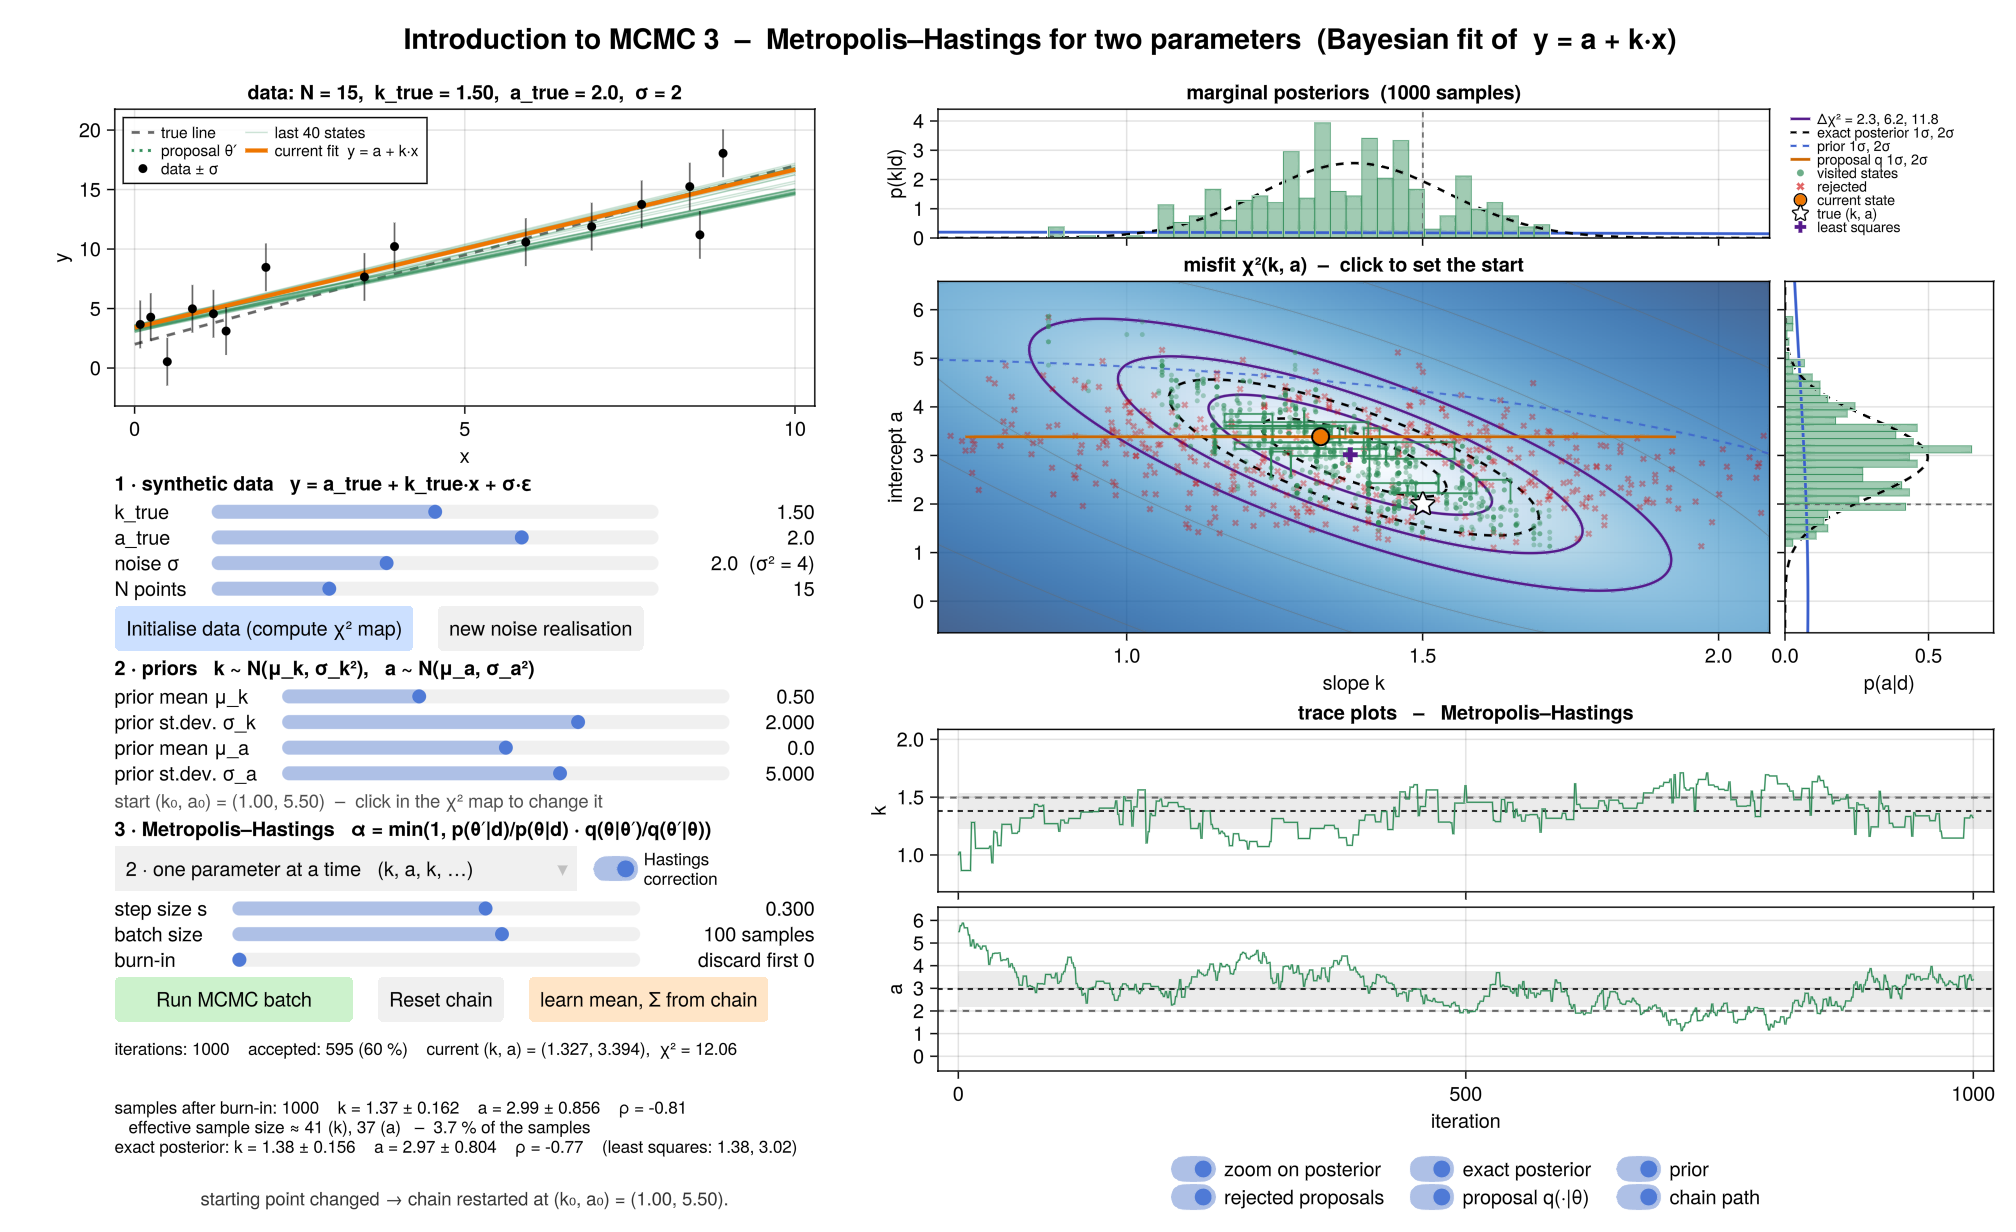
\includegraphics[width=0.49\textwidth]{figures/mcmc3_one_at_a_time.png}\hfill
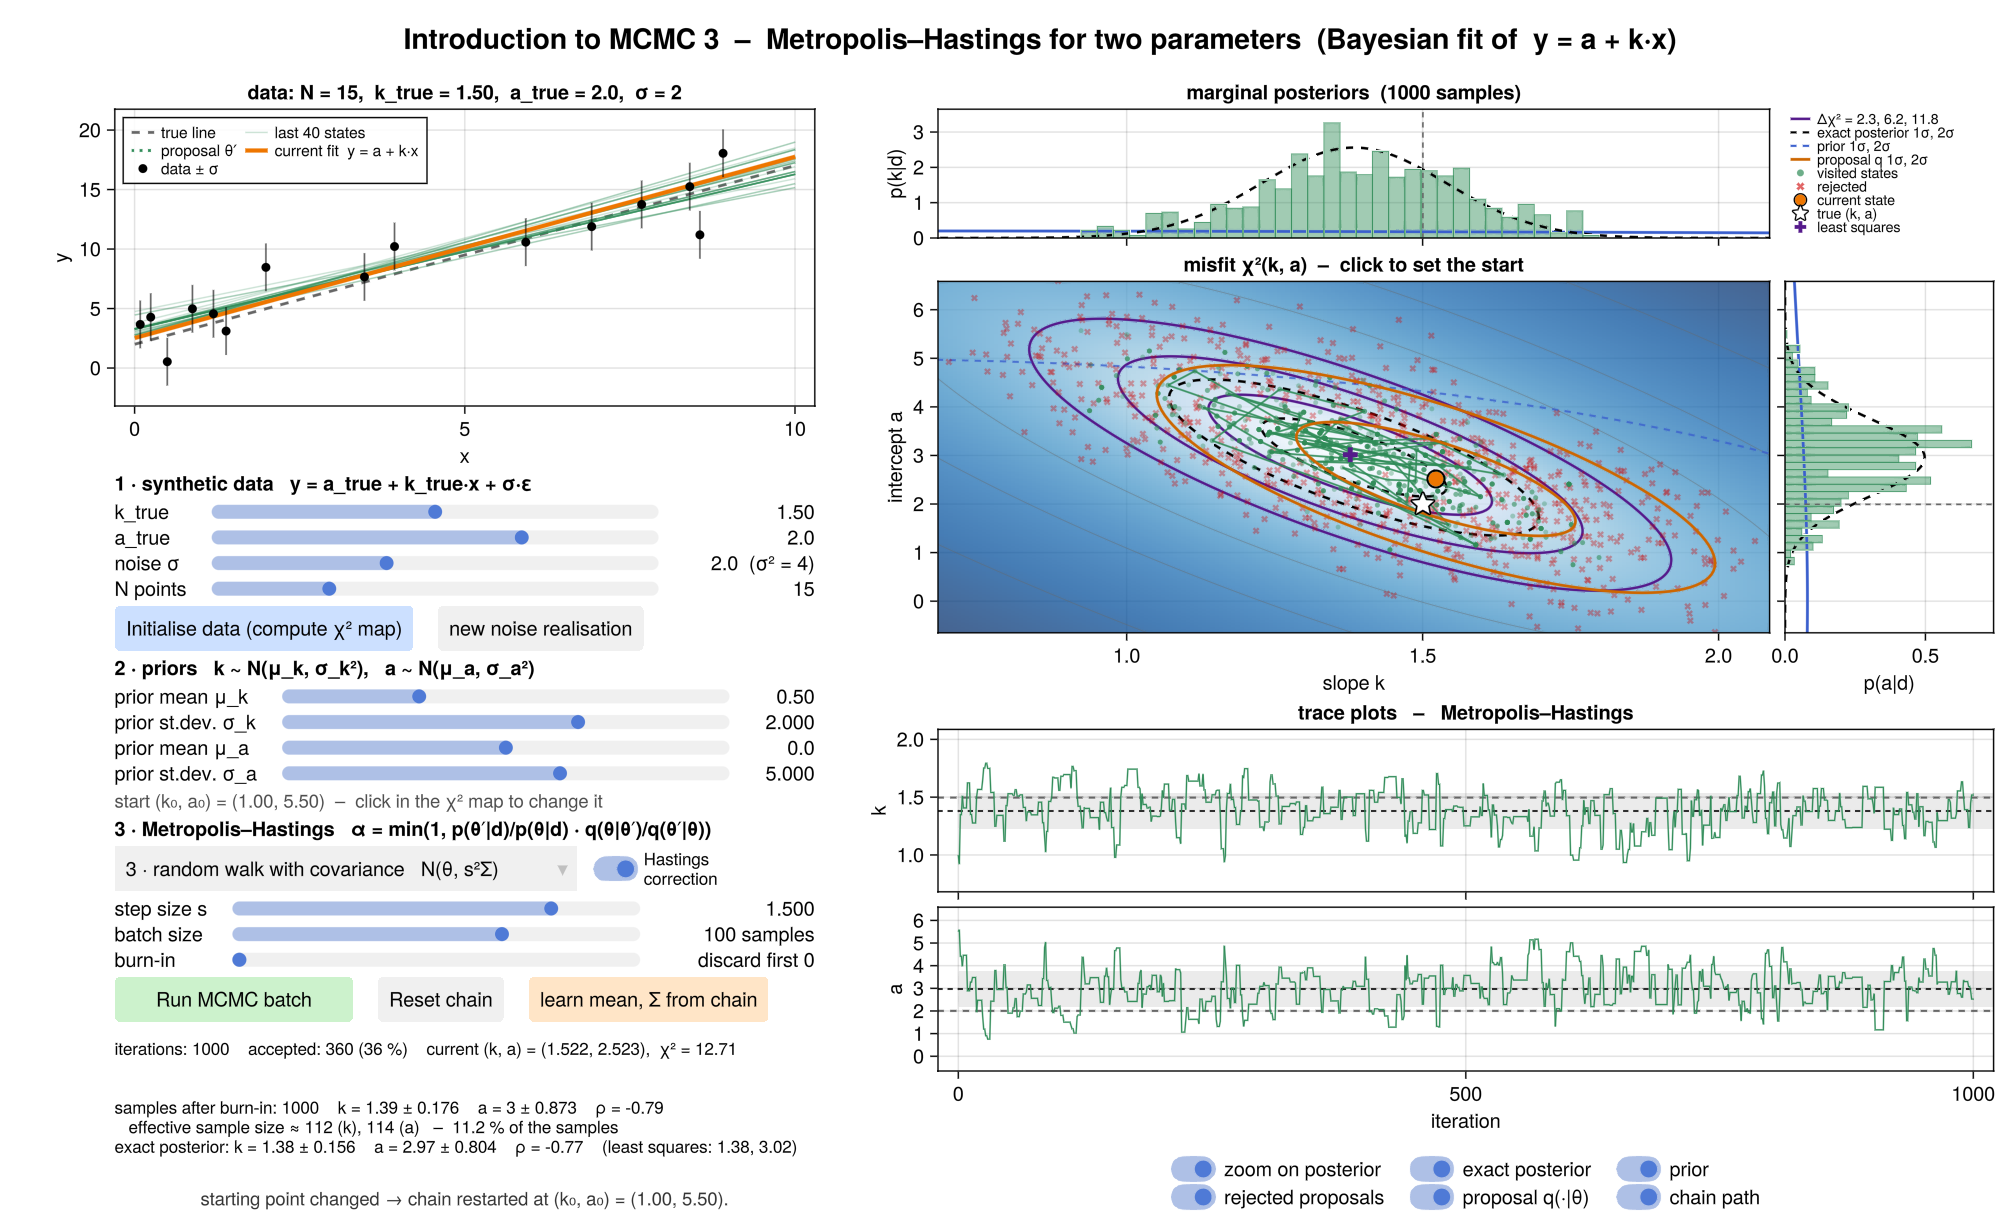
\includegraphics[width=0.49\textwidth]{figures/mcmc3_learned.png}
\caption{1000 iterations from $(1.0,5.5)$, zoomed. Left: one parameter at a time ($s=0.3$): the path consists of
horizontal and vertical steps (orange cross: the next 1-D step), which are poorly suited to a tilted valley; ESS
41 and 37 (3.7\,\%). Right: random walk with the covariance learned from a pilot run of 3000 iterations
($s=1.5$): the orange proposal ellipses have the shape of the posterior, the chain crosses it in a few steps;
ESS 112 and 114 (11\,\%), about three times more for the same number of iterations (longer runs give a factor
of about seven).}
\end{figure}

\begin{figure}[H]
\centering
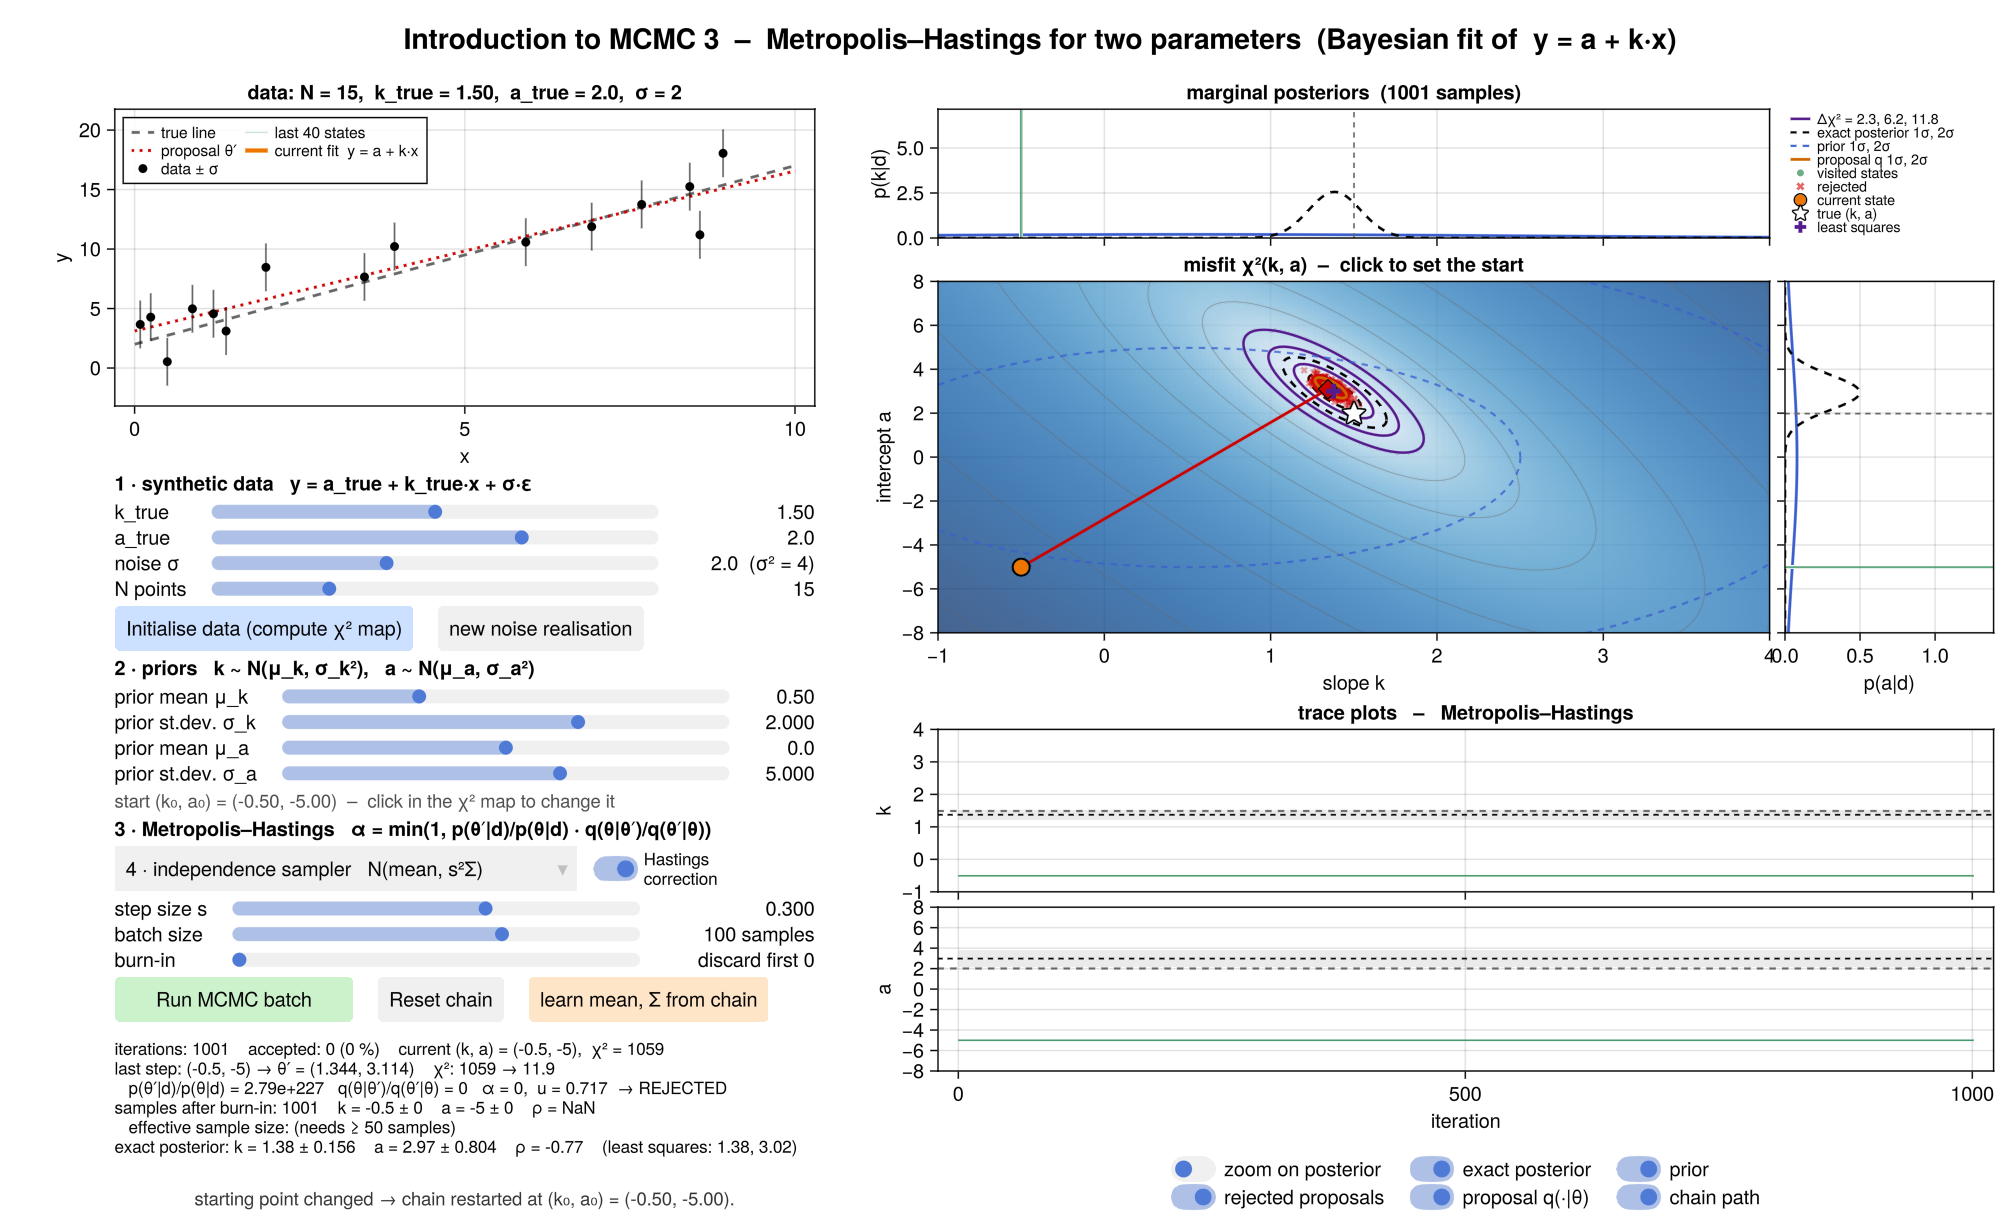
\includegraphics[width=0.6\textwidth]{figures/mcmc3_indep_stuck.png}
\caption{A failure worth remembering: the independence sampler with a narrow proposal ($s=0.3$) started far
away at $(-0.5,-5)$. The proposal $\vth'=(1.34,3.11)$ is excellent (posterior ratio $2.8\times10^{227}$), but
$q(\vth)$ at the starting point is so small that the Hastings ratio $q(\vth)/q(\vth')$ is zero: 1000 iterations,
not a single acceptance. An independence proposal must be \emph{wider} than the posterior ($s\gtrsim1.5$), its
tails must not be too light.}
\end{figure}

\begin{tryit}
\begin{itemize}
\item Compare the ESS of proposals 1 and 2 for the same number of iterations. Why is ``one at a time'' not
  better than the isotropic walk here?
\item Run a pilot of 2000--3000 iterations with proposal 1, set a burn-in, press \btn{learn mean, $\Sigma$ from chain},
  switch to proposal 3 and try $s=1$, 1.5, 2 and 3. Which $s$ gives the largest ESS? (Theory:
  $s\approx2.4/\sqrt{2}\approx1.7$, acceptance $\approx35\,\%$.)
\item Proposals 4 and 5 with the Hastings correction off: what happens to the posterior standard deviations?
\item Make the prior of $a$ narrow ($\sigma_a=0.5$): how do the posterior ellipse and the correlation change?
\end{itemize}
\end{tryit}

%==============================================================================
\clearpage
\section{Program 4 – Hamiltonian Monte Carlo for one parameter}\label{sec:h1}
%==============================================================================
\textbf{File:} \file{Introduction\_HMC\_1.jl}.\quad Fit of $y=k\,x$ with HMC (Section~\ref{sec:hmc}). The upper
right is split in two: the misfit with the last trajectory drawn on it (the particle rolling in the bowl), and
the \textbf{phase space} $(k,p)$ with contours of $H$, the last 25 trajectories (green: accepted, red dashed:
rejected) and the momentum refreshes (vertical dotted jumps at fixed $k$). An HMC chain alternates between
these two moves: along a contour of $H$, then vertically to a new contour.

\begin{figure}[H]
\centering
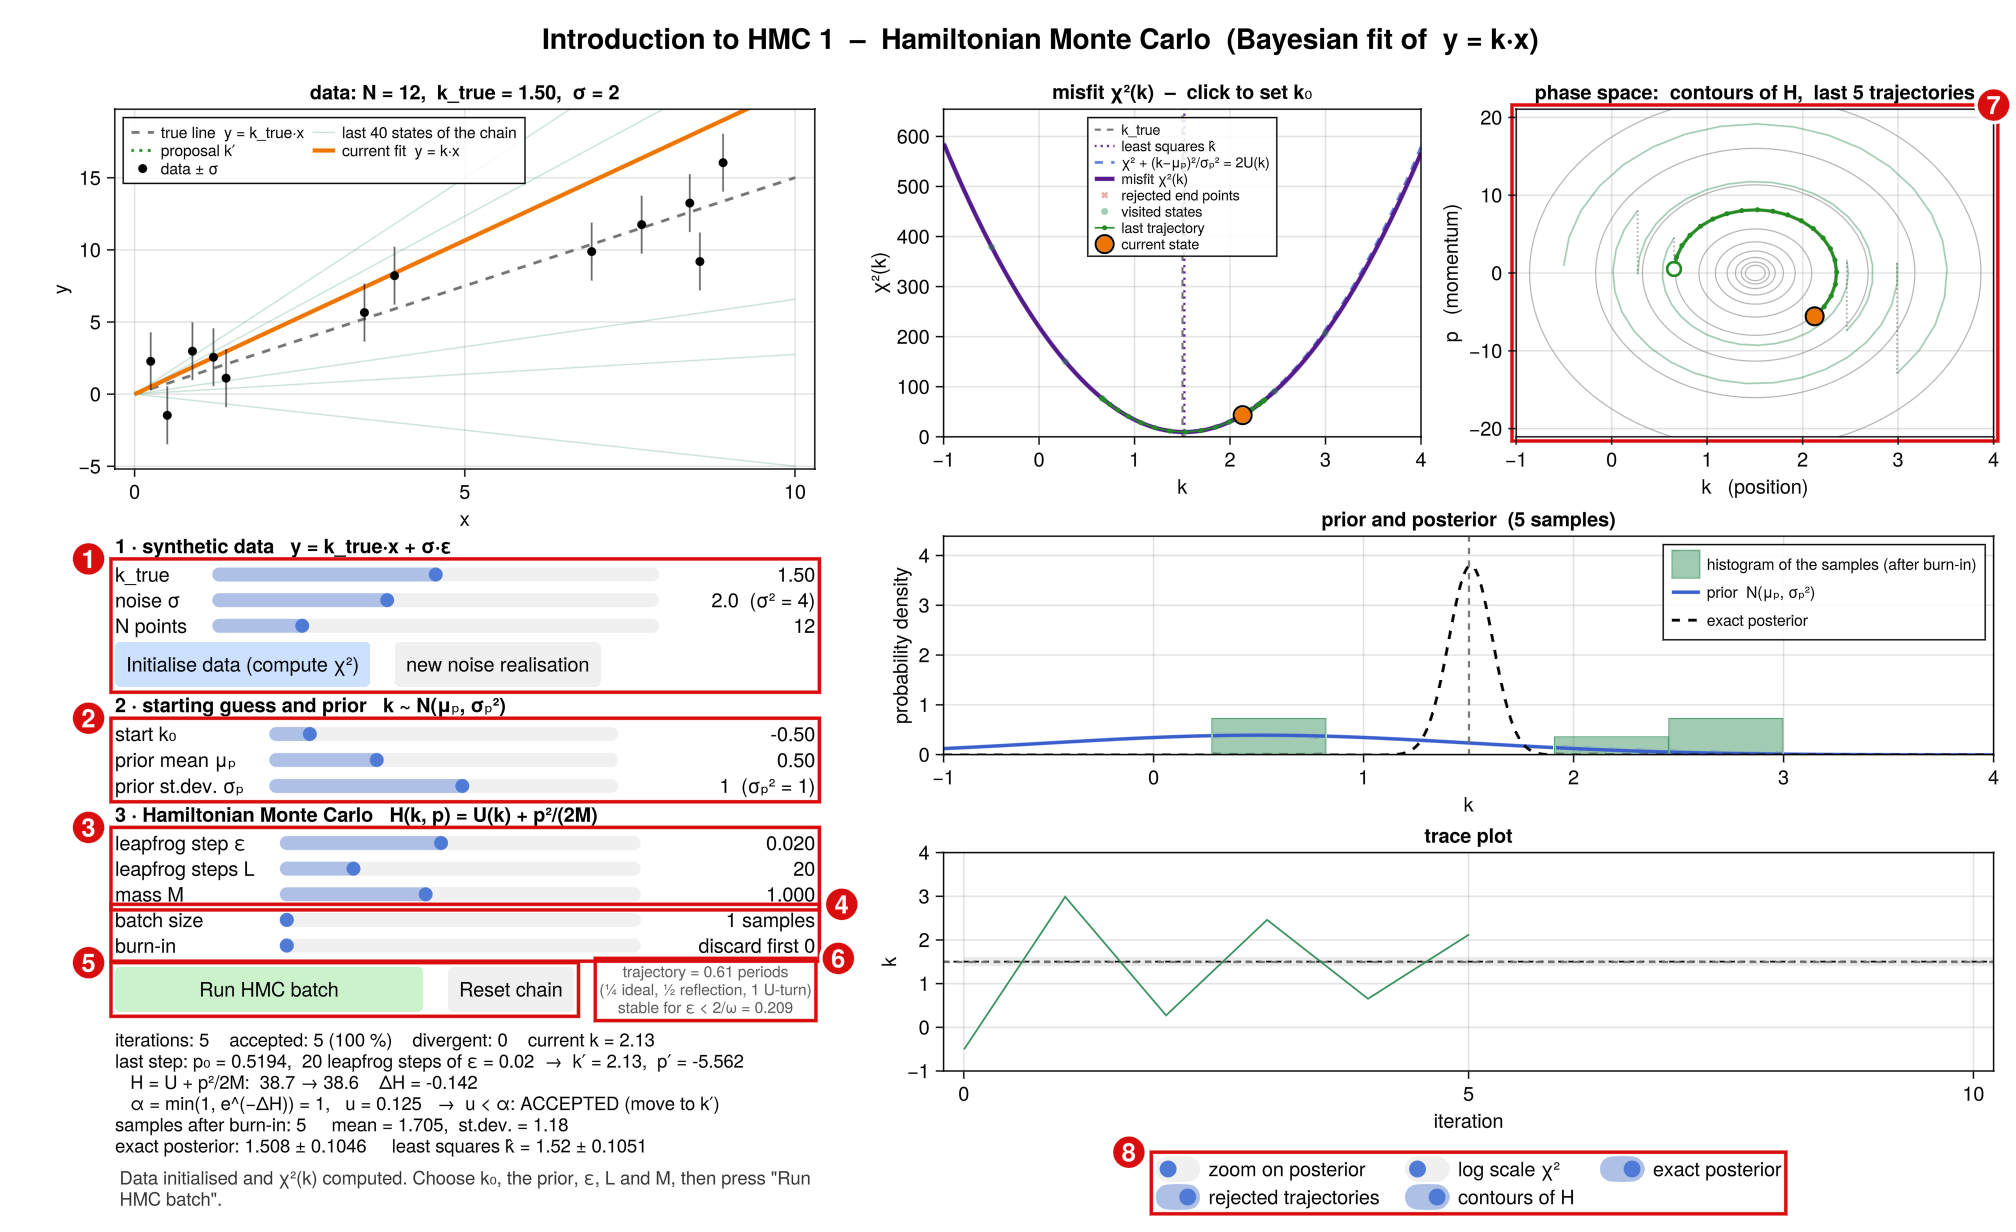
\includegraphics[width=\textwidth]{figures/hmc1_overview.png}
\caption{Program 4 after five single iterations from $k_0=-0.5$ ($\varepsilon=0.02$, $L=20$, $M=1$; trajectory
= 0.61 periods). The start is high in the bowl ($H\approx40$, the bottom is at $\approx5$): the first trajectories
swing across the whole valley (trace: $-0.5\to3\to0.3\to2.4\dots$) and energy is lost only through the momentum
refreshes, visible as the spiral in phase space. Last step: $p_0=0.52$, $k'=2.13$, $\Delta H=-0.14$, accepted.}
\label{fig:h1}
\end{figure}

\paragraph{Step by step} (numbers as in Fig.~\ref{fig:h1})
\begin{enumerate}[label=\protect\step{\arabic*}]
\item Data and \btn{Initialise data (compute $\chi^2$)}, as in Program~1.
\item Starting guess and prior; a click in the misfit panel sets $k_0$.
\item The leapfrog step $\varepsilon$, the number of steps $L$ and the mass $M$.
\item Batch size and burn-in.
\item \btn{Run HMC batch}, \btn{Reset chain}. With a batch of 1 the info text lists $p_0$, the end point
  $(k',p')$, $H$ before and after, $\Delta H$, $\alpha=\min(1,e^{-\Delta H})$ and $u$.
\item The trajectory length in oscillation periods of the leapfrog
  (Section~\ref{sec:osc}; $\tfrac14$ ideal, $\tfrac12$ reflection, 1 U-turn) and the stability limit
  $\varepsilon<2/\omega$. It turns orange near $\tfrac12$ or 1 period and red when $\varepsilon$ is unstable.
\item The phase-space panel.
\item Toggles, including \ctl{contours of H}.
\end{enumerate}

\begin{figure}[H]
\centering
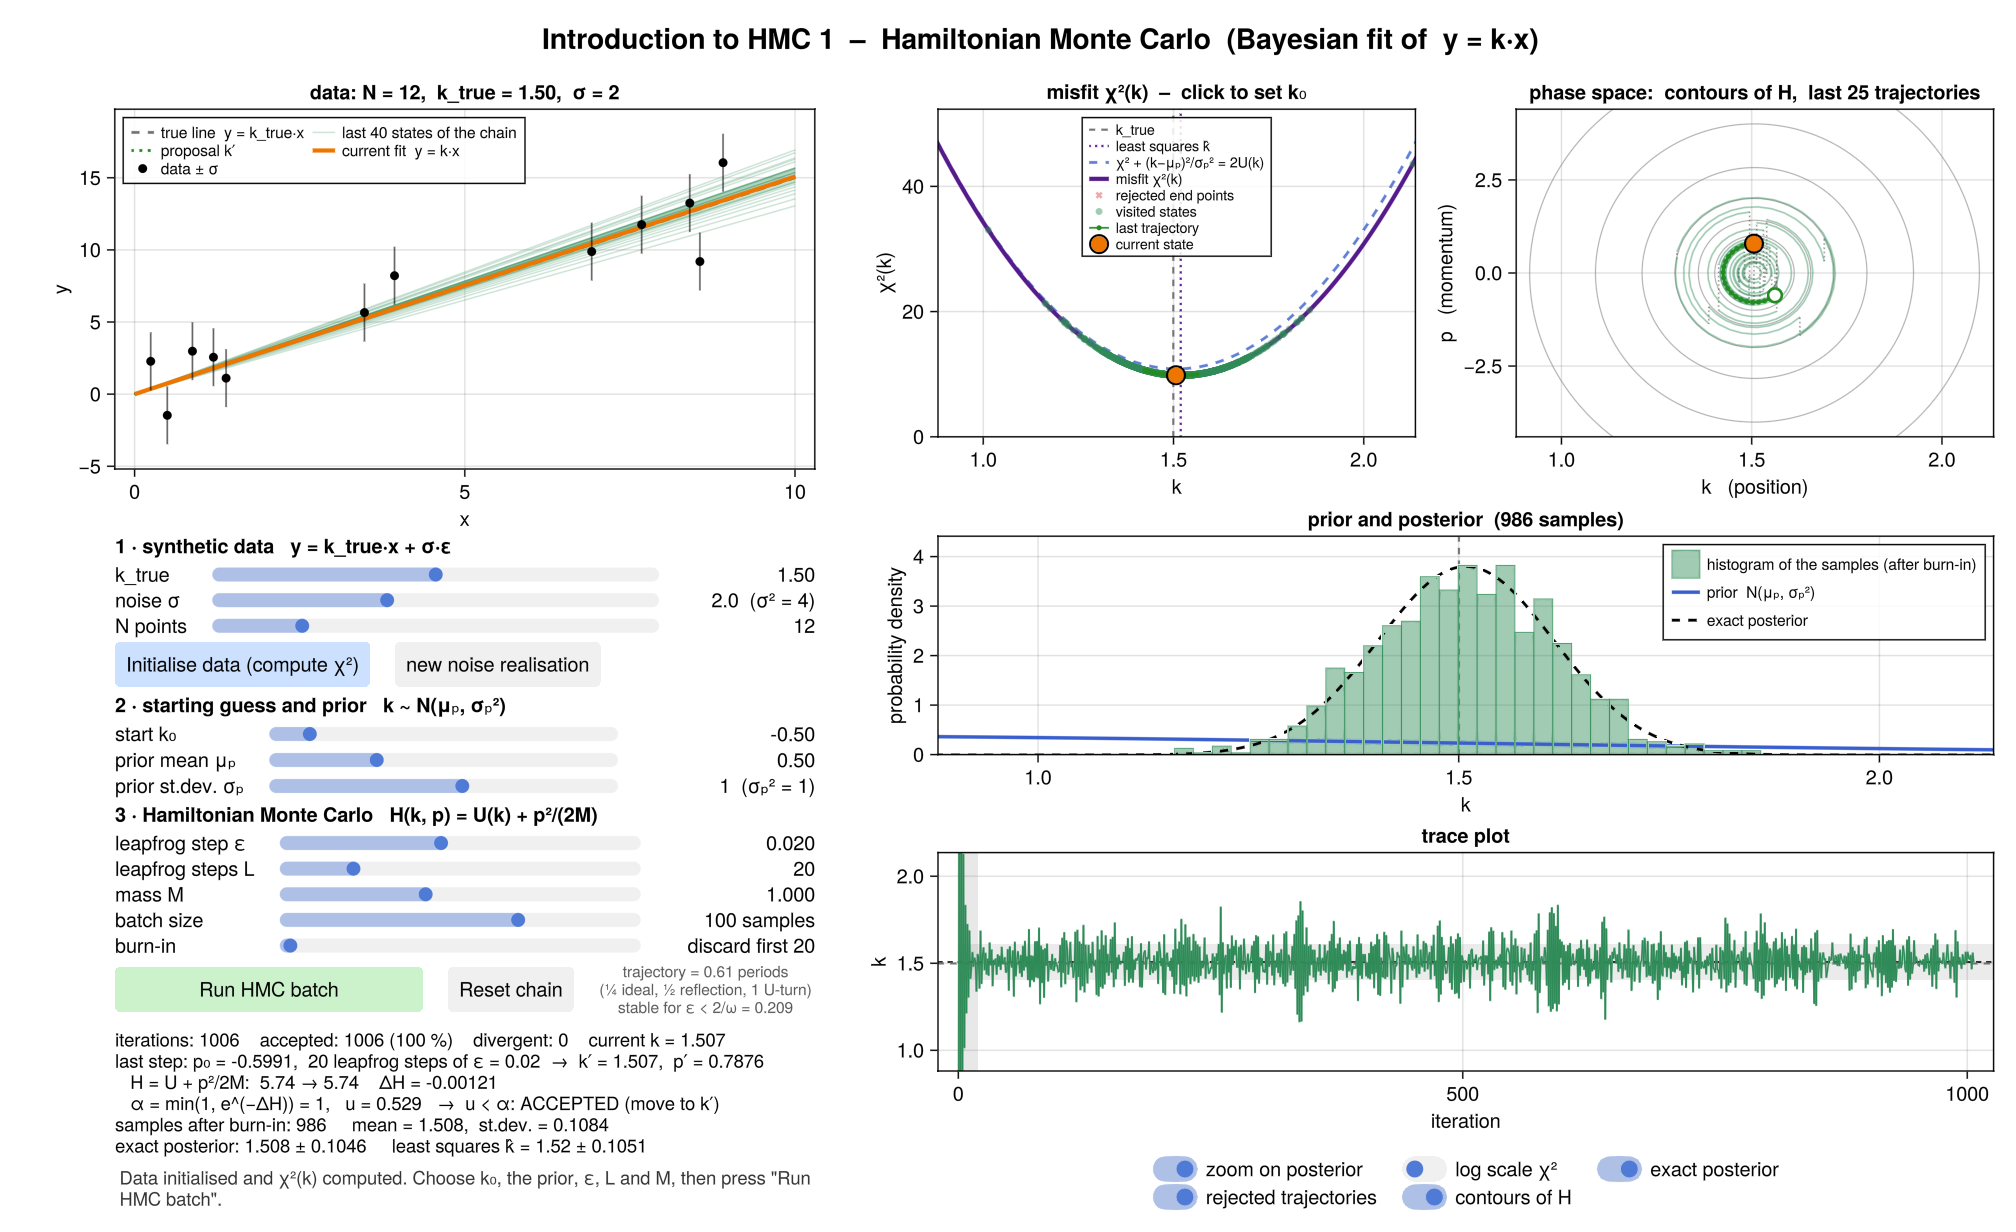
\includegraphics[width=0.49\textwidth]{figures/hmc1_converged.png}\hfill
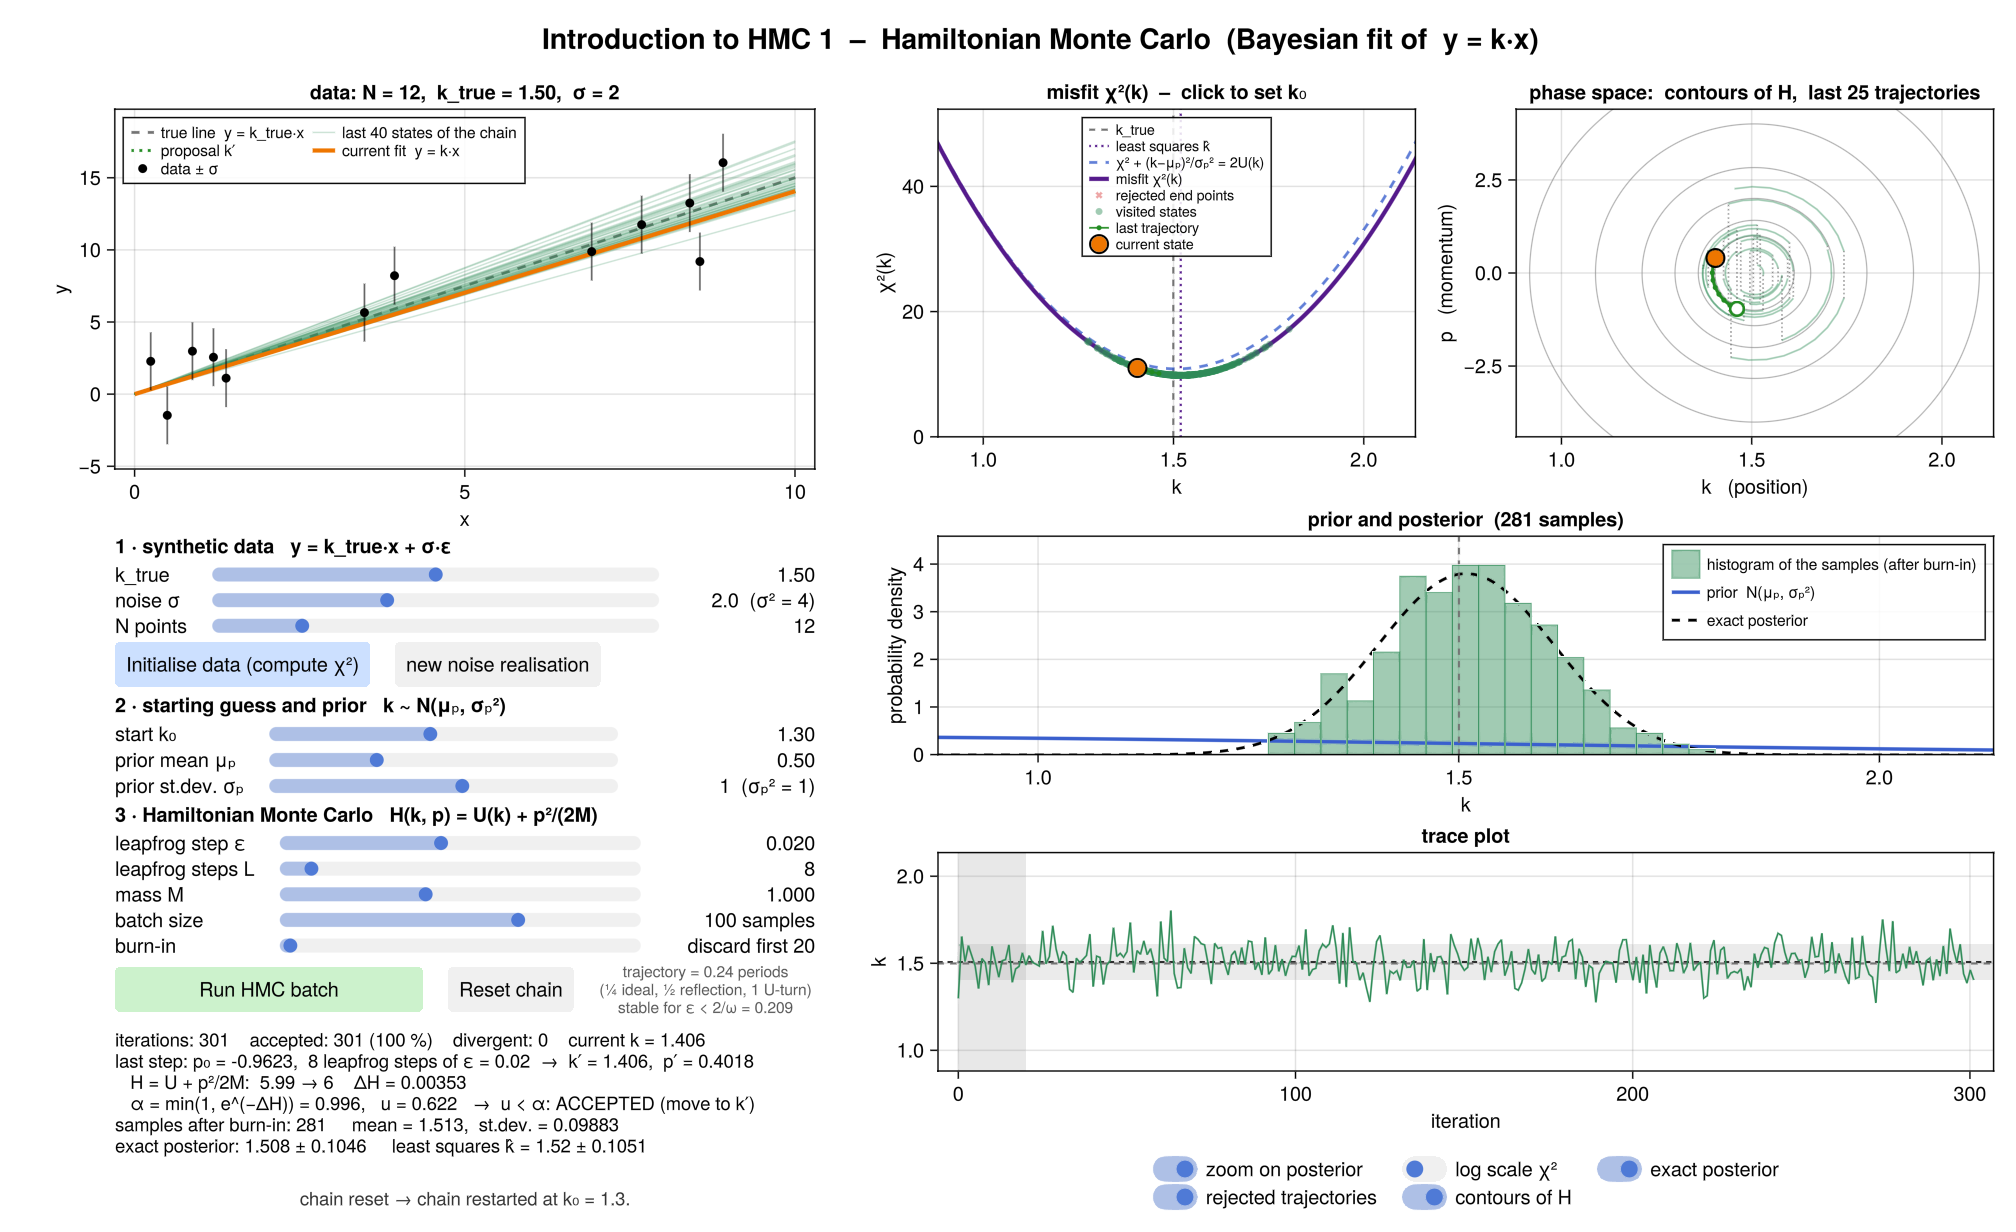
\includegraphics[width=0.49\textwidth]{figures/hmc1_quarter.png}
\caption{Left: 1000 iterations with the default settings, zoomed: all trajectories accepted, the trajectories
are ellipses around the bottom of the bowl; burn-in 20: $k=1.508\pm0.108$ (exact $1.508\pm0.105$). With 0.61
periods each sample lands roughly on the opposite side of the posterior (anti-correlated trace). Right:
$L=8$, a quarter period: nearly independent samples, 300 iterations give $k=1.513\pm0.098$.}
\end{figure}

\begin{figure}[H]
\centering
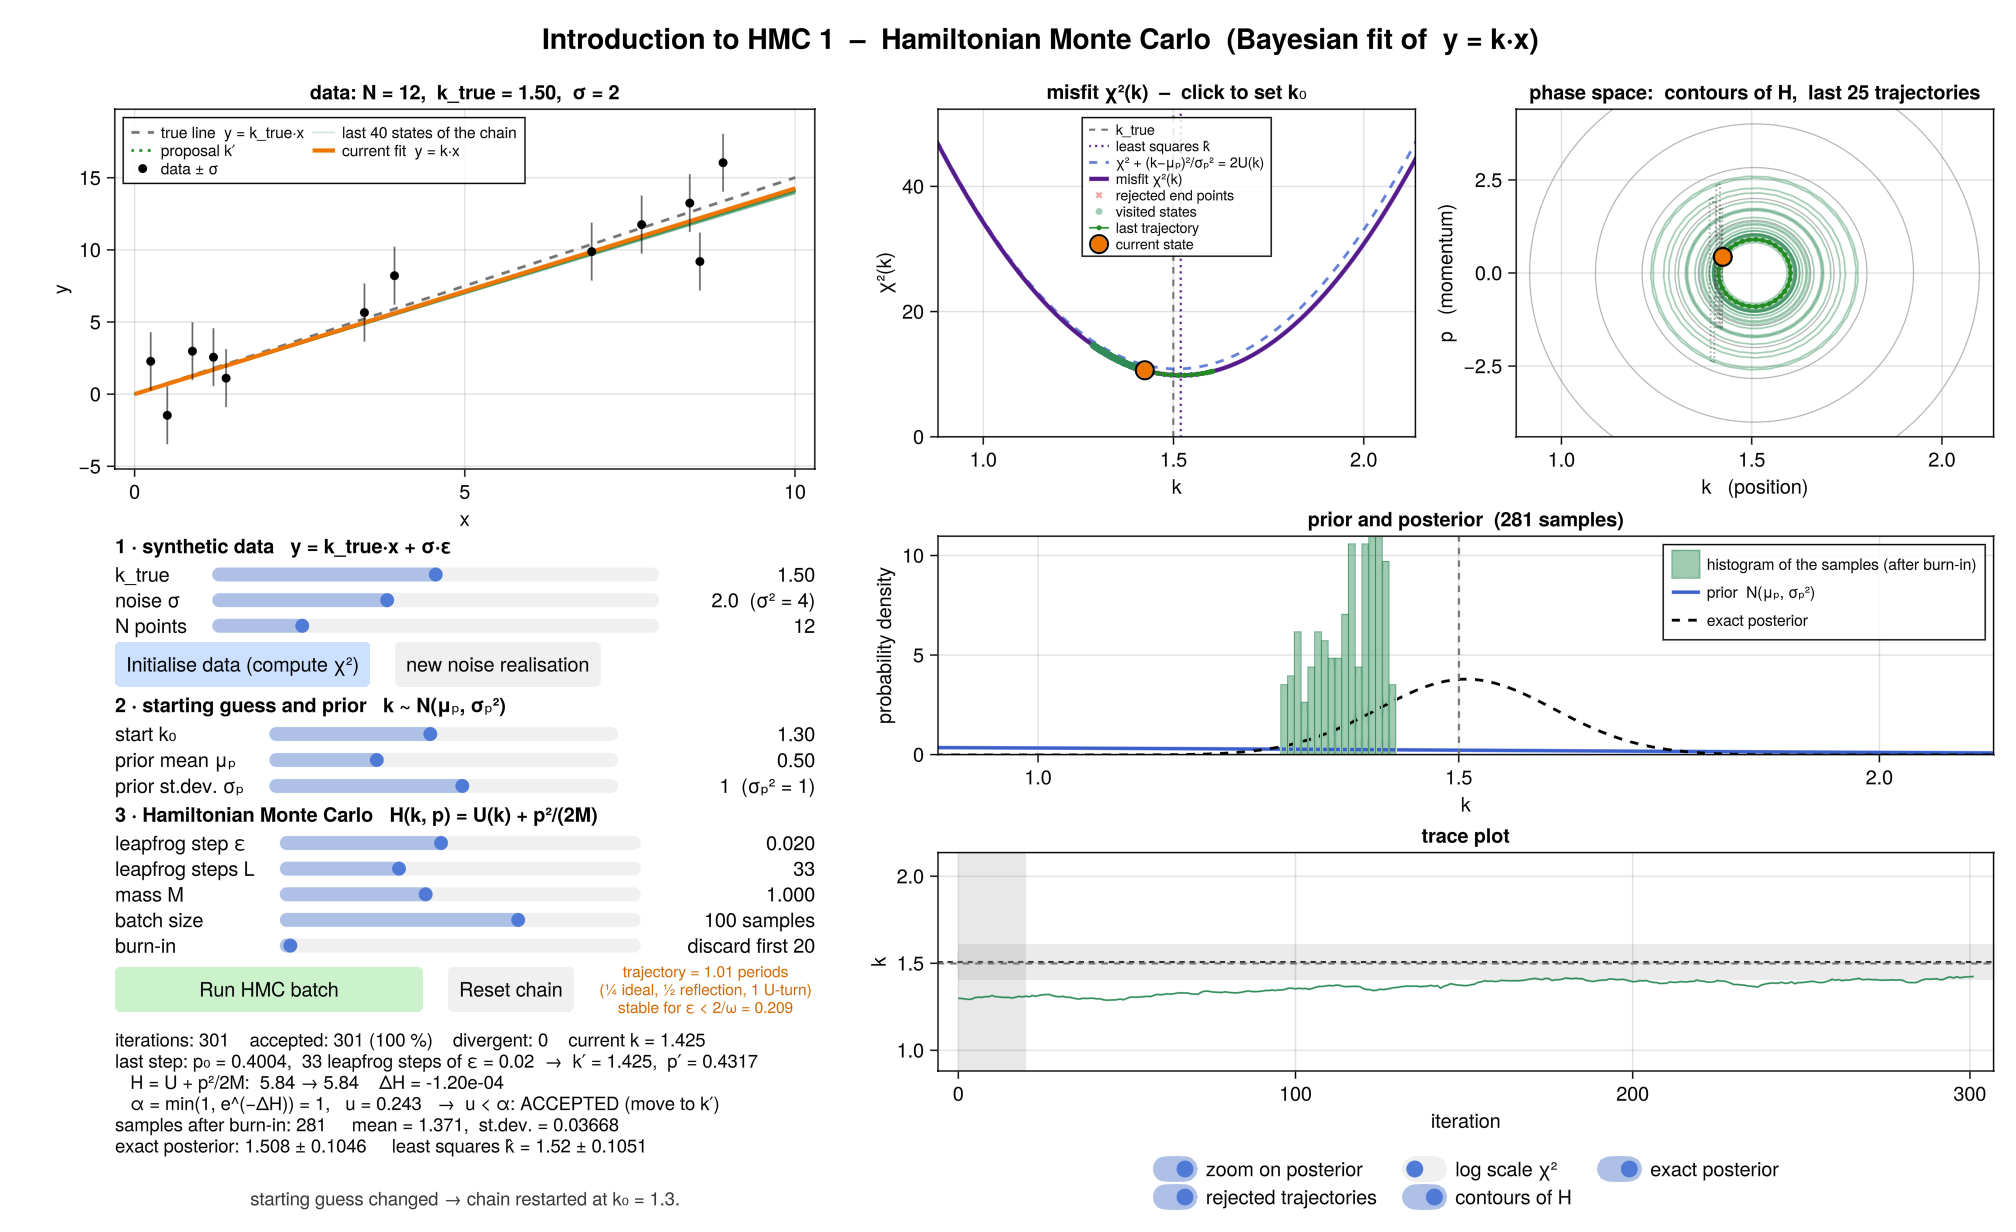
\includegraphics[width=0.49\textwidth]{figures/hmc1_uturn.png}\hfill
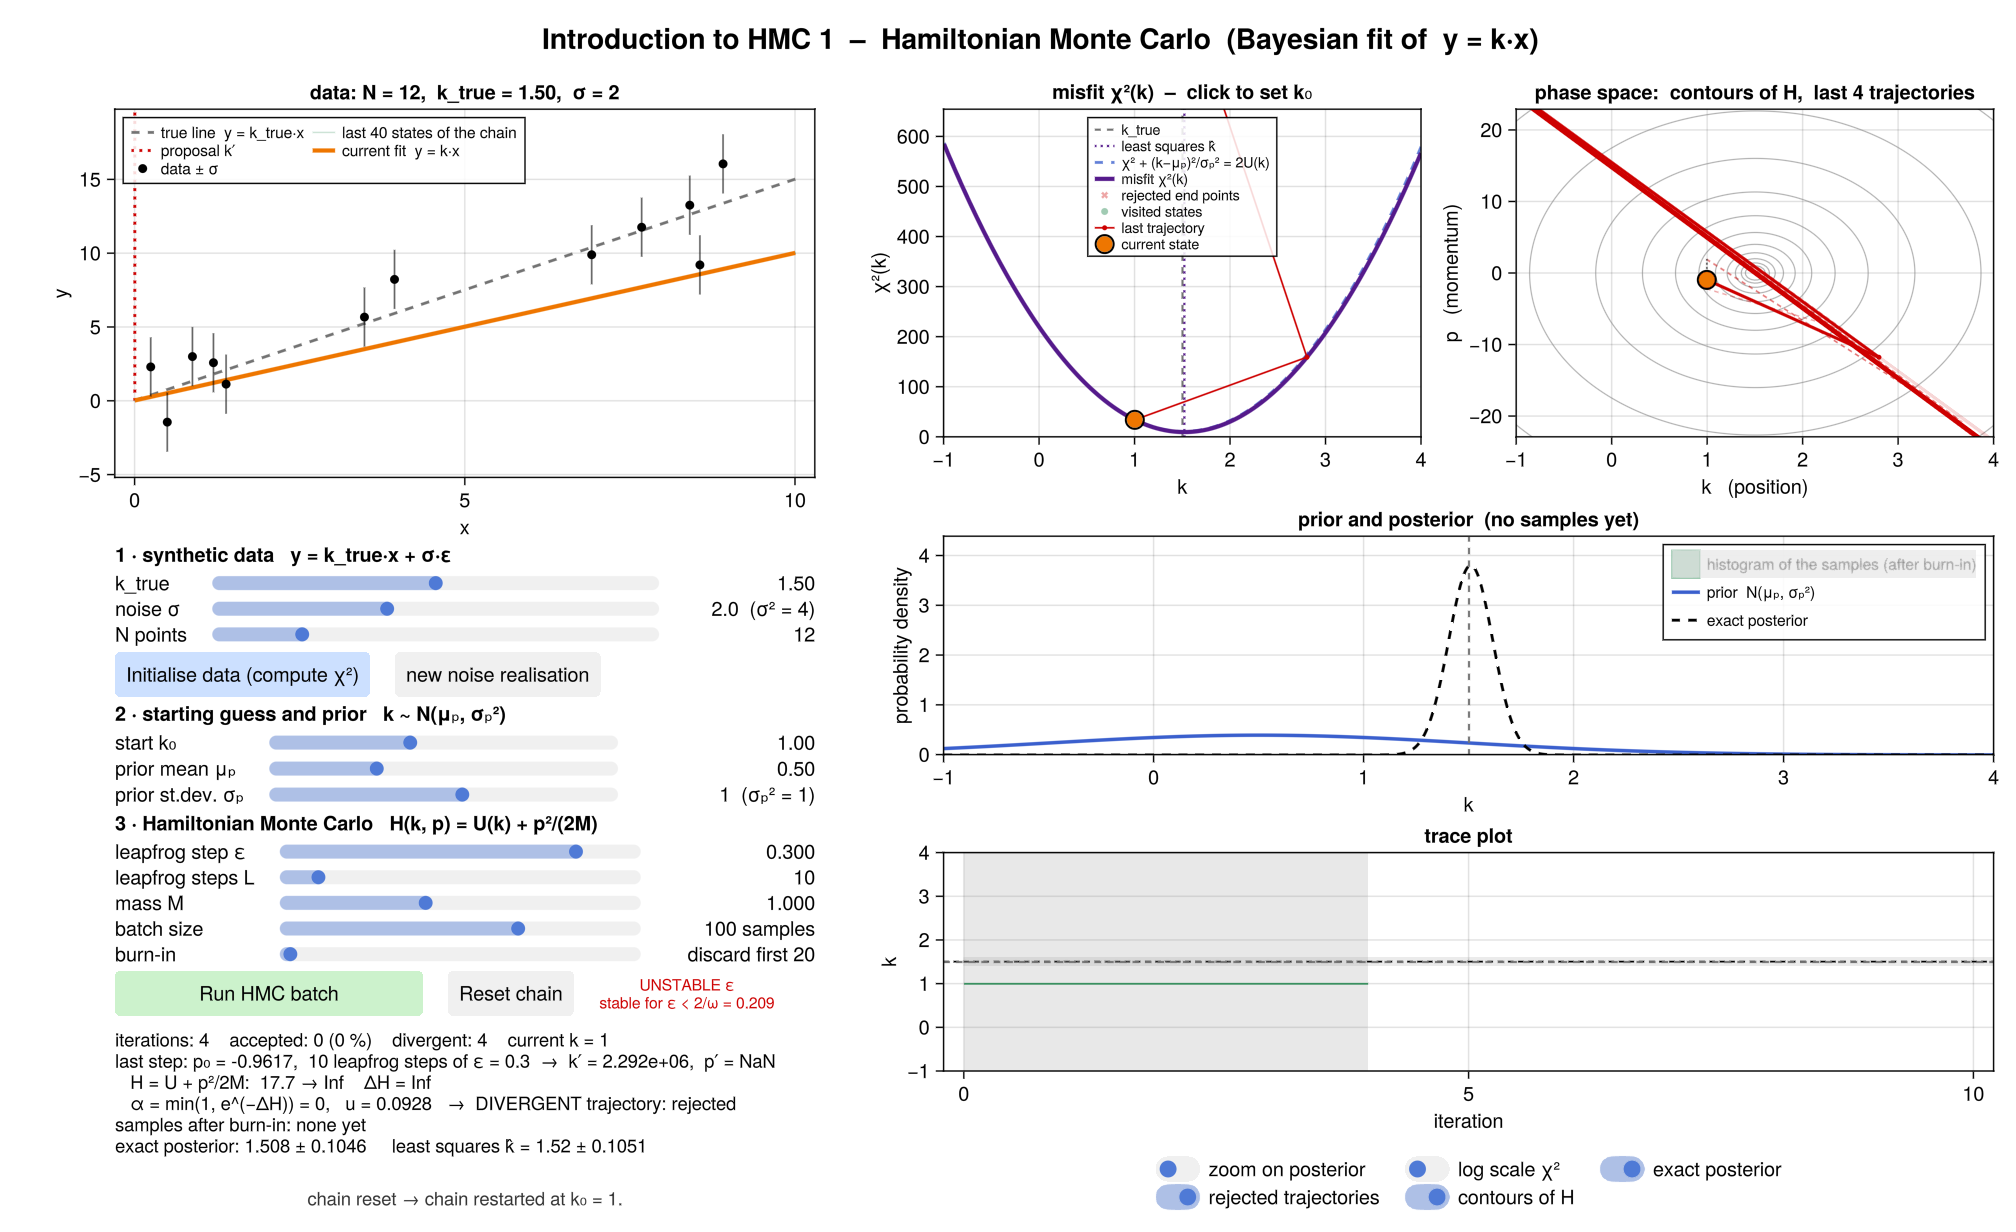
\includegraphics[width=0.49\textwidth]{figures/hmc1_unstable.png}
\caption{Left: $L=33$, the trajectory is one full period (warning in orange): every trajectory is a closed
circle in phase space and returns to its start (U-turn). Everything is accepted, but after 300 iterations from
$k_0=1.3$ the chain has barely moved: $k=1.371\pm0.037$. Right: $\varepsilon=0.3$, above the stability limit
0.209 (warning in red): the leapfrog scheme blows up, every trajectory diverges (red straight lines leaving the
panel; $k'=2.3\times10^6$, $\Delta H=\infty$) and is rejected.}
\end{figure}

\begin{tryit}
\begin{itemize}
\item With a batch of 1, compare $\Delta H$ for $\varepsilon=0.01$, 0.05 and 0.15. How does the acceptance
  change, and why does it stay high even for fairly large $\varepsilon$?
\item Keep $L\varepsilon$ fixed (e.g.\ $\varepsilon=0.01$, $L=40$ and $\varepsilon=0.04$, $L=10$): is the
  trajectory the same? What costs more computing time?
\item Find $L$ for $\tfrac14$, $\tfrac12$ and 1 period and compare the trace plots.
\item Increase the mass to $M=100$: the oscillation becomes ten times slower. Which $\varepsilon$ is now
  stable?
\end{itemize}
\end{tryit}

%==============================================================================
\clearpage
\section{Program 5 – Hamiltonian Monte Carlo for two parameters}\label{sec:h2}
%==============================================================================
\textbf{File:} \file{Introduction\_HMC\_2.jl}.\quad Fit of $y=a+k\,x$ with HMC. Phase space is now
four-dimensional $(k,a,p_k,p_a)$; the program shows the trajectories in \emph{parameter space} on the misfit map
and two projections of phase space, $(k,p_k)$ and $(a,p_a)$, each with the momentum refreshes. The mass matrix
can be the identity, diagonal ($M=\mathrm{diag}(1/\mathrm{var}_k,1/\mathrm{var}_a)$) or full ($M=\hat\Sigma^{-1}$),
with $\hat\Sigma$ learned from a pilot run as in Program~3.

\begin{figure}[H]
\centering
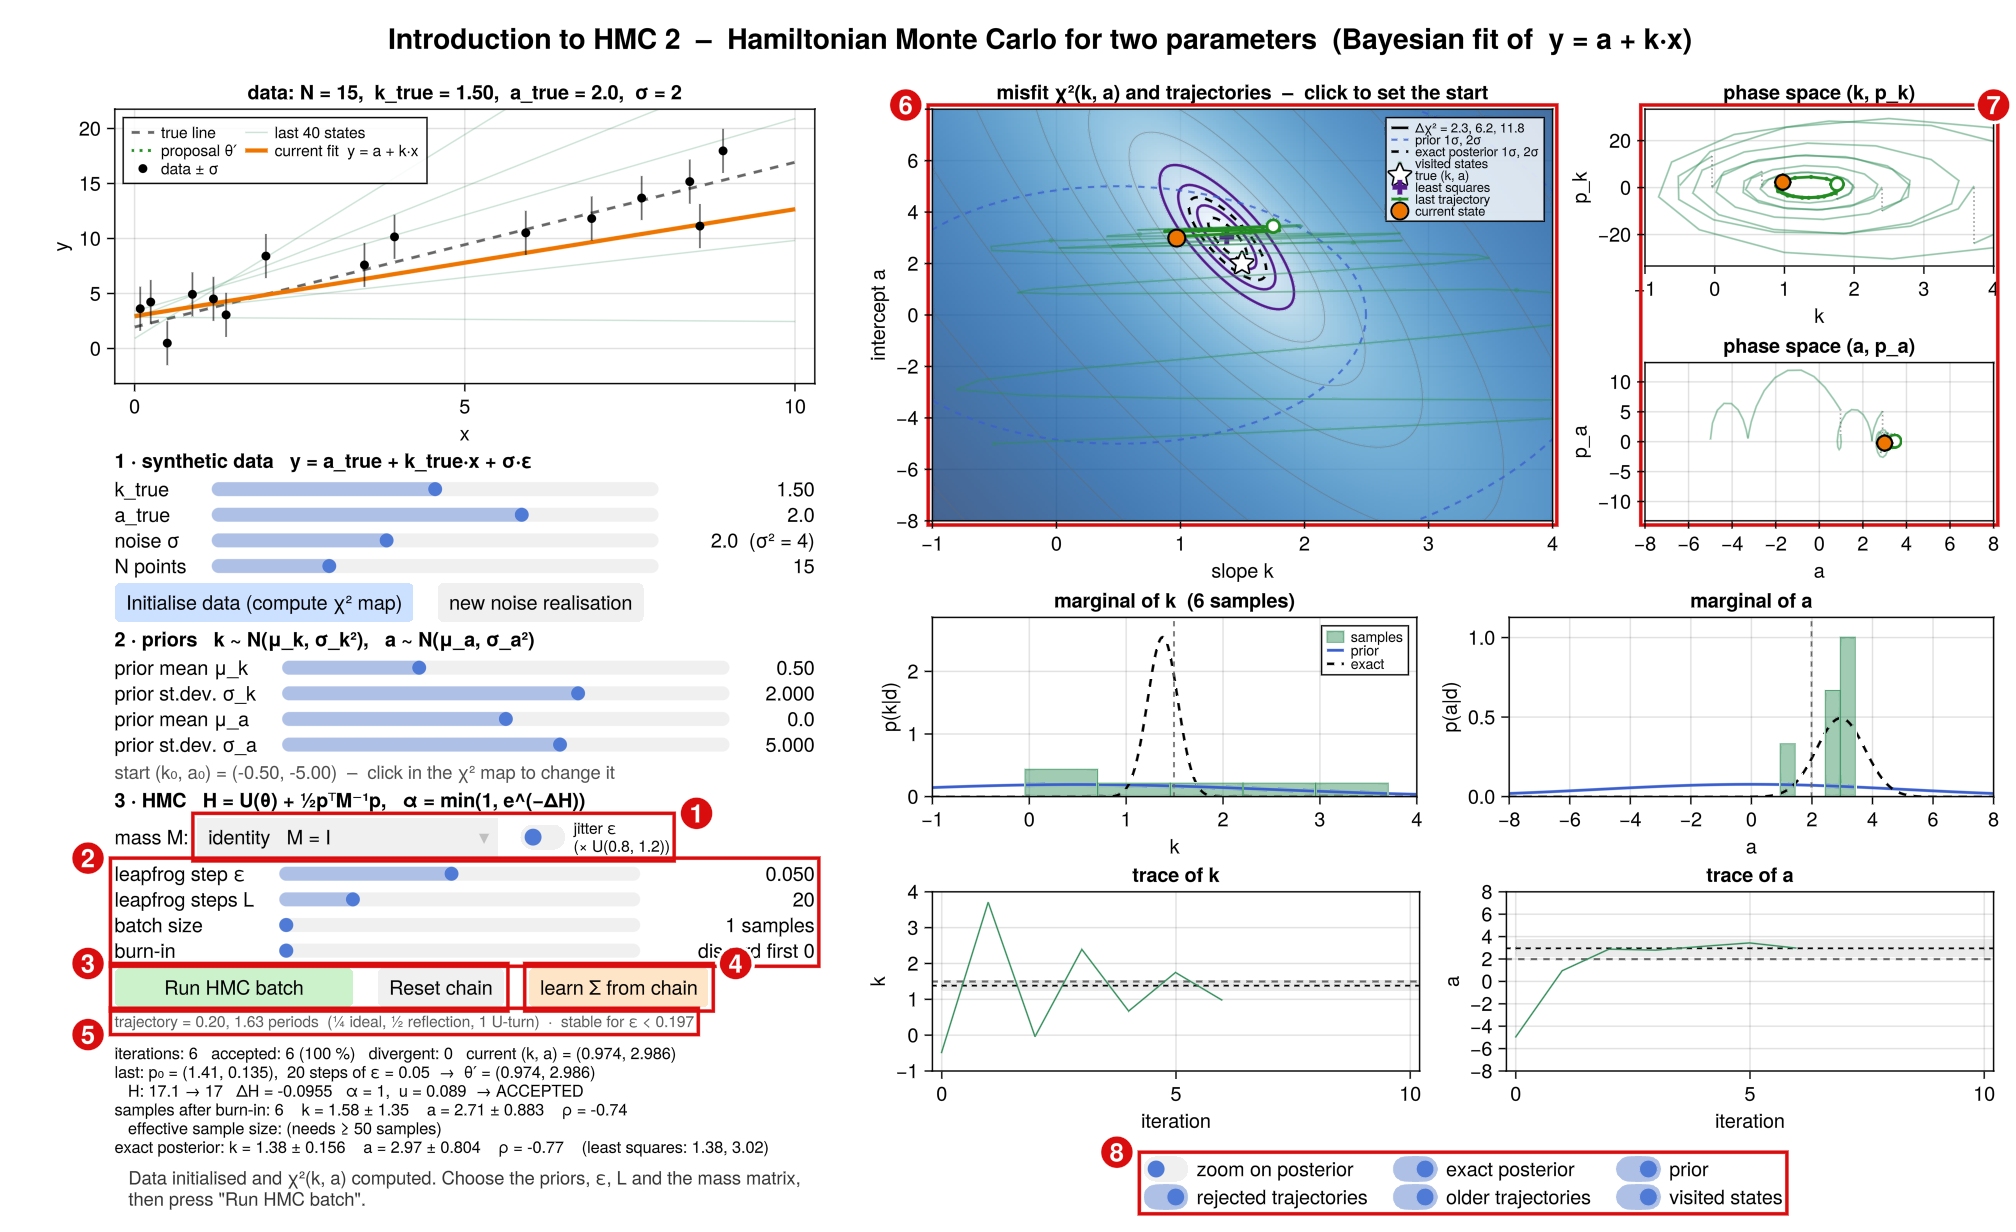
\includegraphics[width=\textwidth]{figures/hmc2_overview.png}
\caption{Program 5 after six single iterations from $(-0.5,-5)$ with $M=I$, $\varepsilon=0.05$, $L=20$. The
trajectories in the map oscillate almost horizontally: the stiff direction of the tilted valley (period 0.62)
is crossed several times per trajectory (1.63 periods), the long direction (period 5.1) only by a fifth of a
period. The stability limit is $\varepsilon<0.197$.}
\label{fig:h2}
\end{figure}

\paragraph{Step by step} (numbers as in Fig.~\ref{fig:h2}; data, priors and starting point as in Program~3)
\begin{enumerate}[label=\protect\step{\arabic*}]
\item The mass matrix and \ctl{jitter $\varepsilon$}: each trajectory uses $\varepsilon\times U(0.8,1.2)$.
\item $\varepsilon$, $L$, batch size, burn-in.
\item \btn{Run HMC batch}, \btn{Reset chain}.
\item \btn{learn $\Sigma$ from chain}: the covariance of the samples after burn-in, for the diagonal and full mass
  matrix. Until it is pressed, $M=I$ is used.
\item The trajectory length in periods of both directions, with a RESONANCE warning (orange) when one of them
  is close to a multiple of half a period, and the stability limit $\varepsilon<2/\omega_\text{max}$.
\item The misfit map with the last trajectory (leapfrog points), the older trajectories, the visited states, the
  prior and exact posterior ellipses.
\item The two phase-space projections.
\item Toggles.
\end{enumerate}

\begin{figure}[H]
\centering
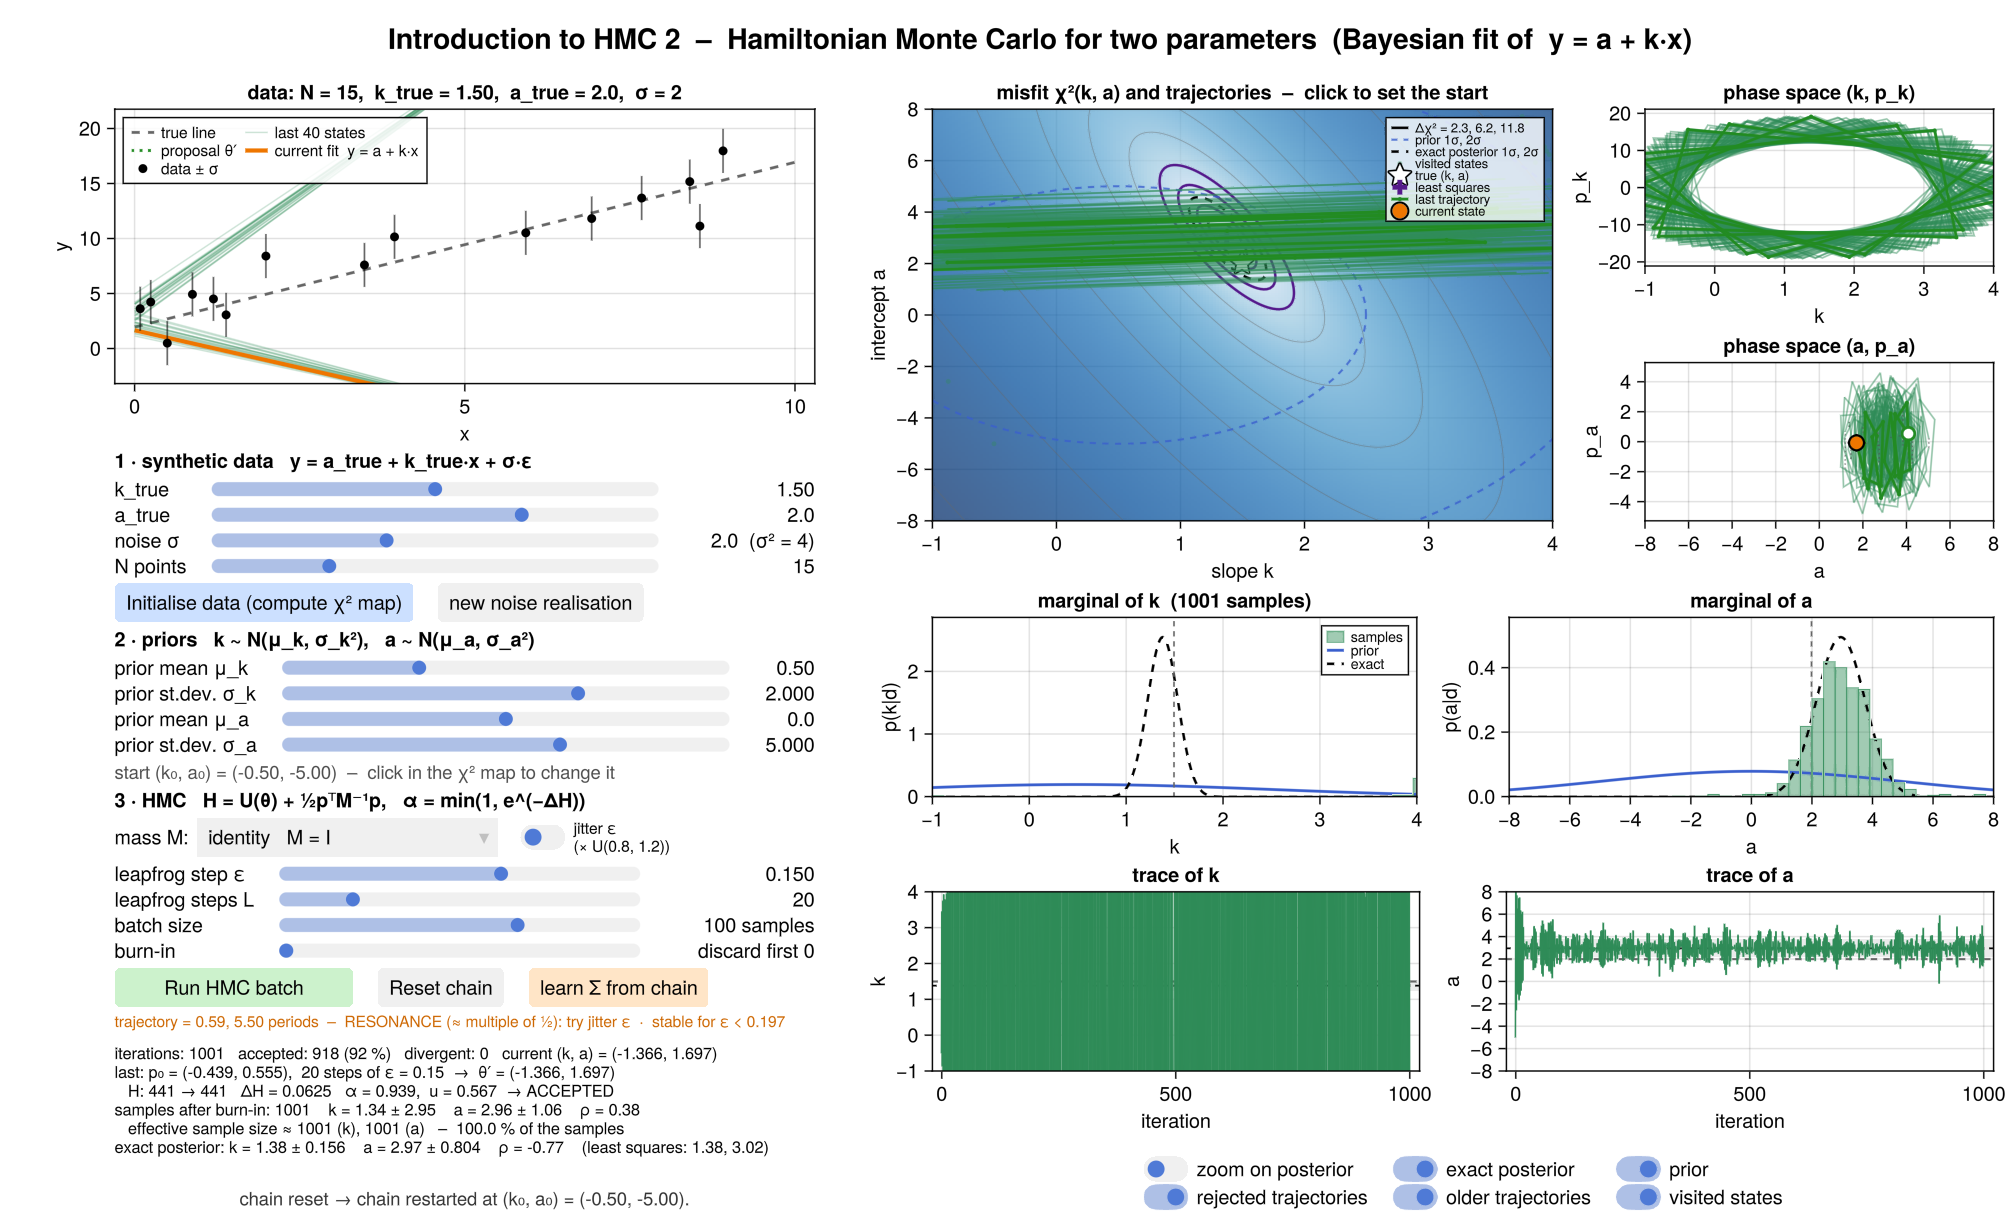
\includegraphics[width=0.49\textwidth]{figures/hmc2_resonance.png}\hfill
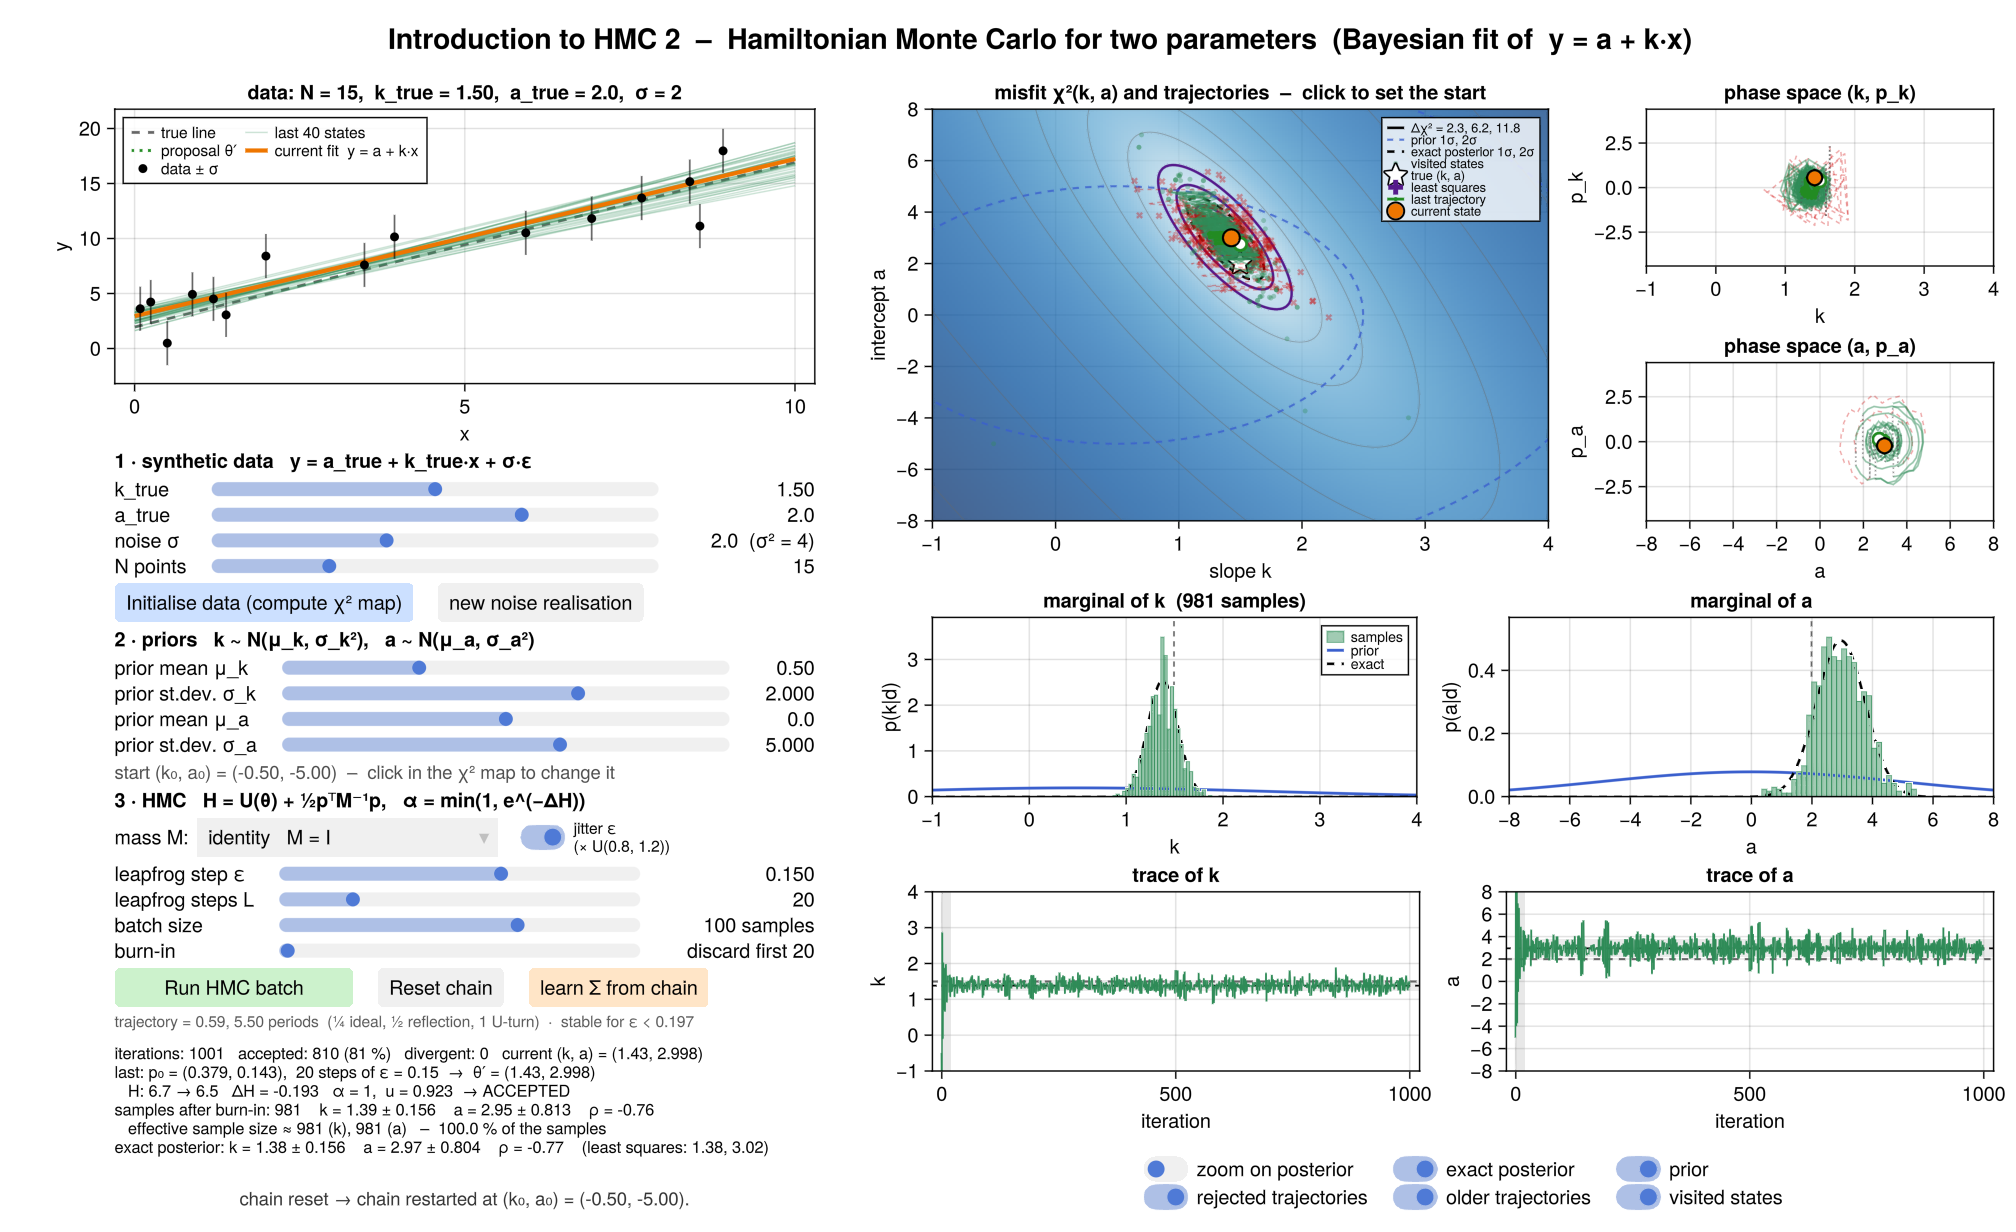
\includegraphics[width=0.49\textwidth]{figures/hmc2_jitter.png}
\caption{Resonance. Left: $M=I$, $\varepsilon=0.15$, $L=20$, 1000 iterations from $(-0.5,-5)$. The stiff
oscillation makes 5.50 periods, a multiple of $\tfrac12$ (orange warning): each trajectory mirrors the stiff
coordinate, the momentum refreshes cannot remove the energy ($H\approx441$, the bottom is at $\approx7$), and the
chain swings across the whole $k$ range: $k=1.34\pm2.95$ instead of $1.38\pm0.156$, although 92\,\% of the
trajectories are accepted and the ESS estimate looks perfect. Right: the same with \ctl{jitter $\varepsilon$}: burn-in after
a few iterations, $k=1.39\pm0.156$, $a=2.95\pm0.813$, $\rho=-0.76$, in agreement with the exact posterior.}
\end{figure}

\begin{figure}[H]
\centering
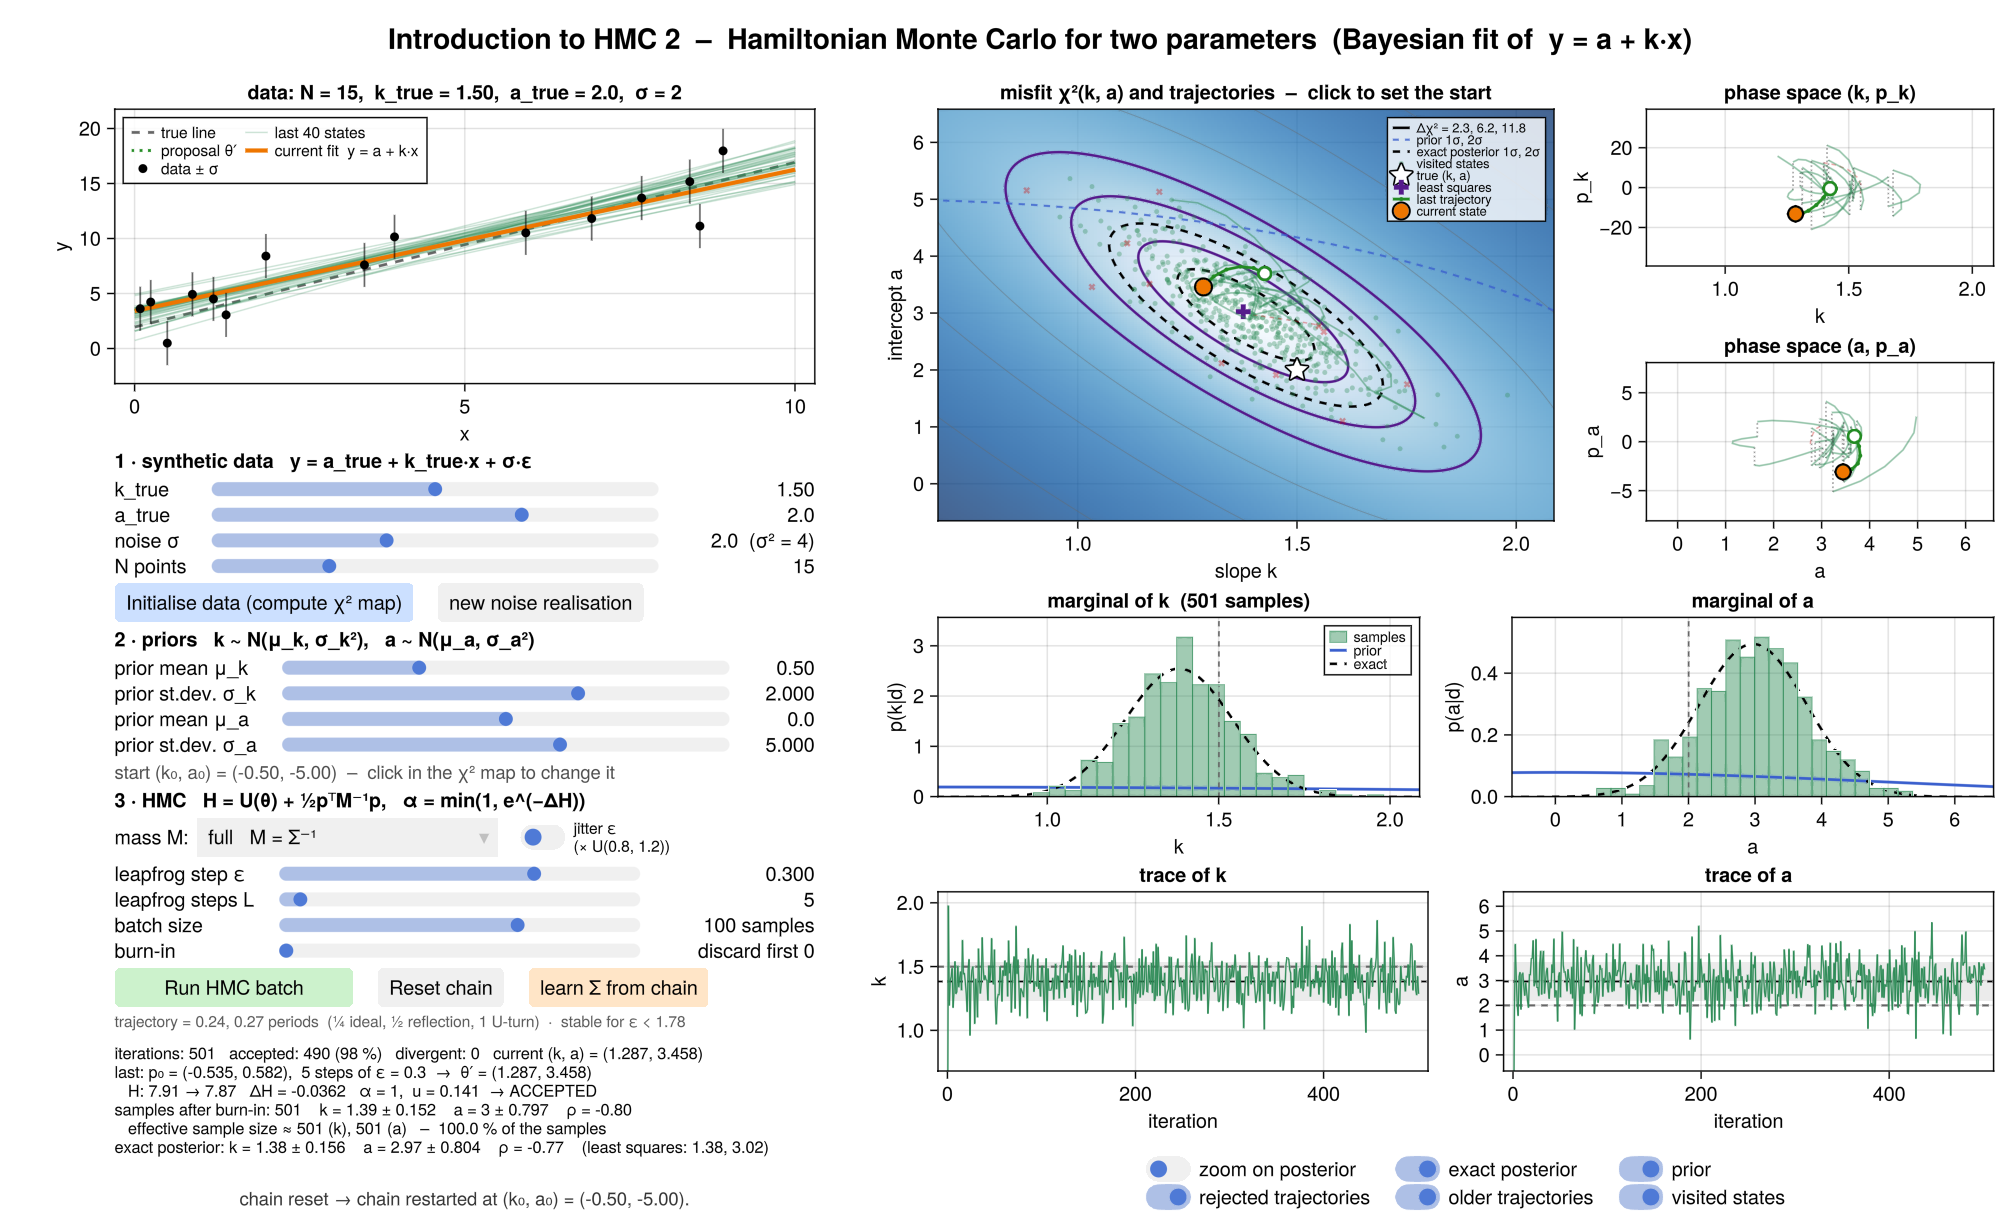
\includegraphics[width=0.6\textwidth]{figures/hmc2_fullmass.png}
\caption{Full mass matrix $M=\hat\Sigma^{-1}$ learned from a pilot run, $\varepsilon=0.3$, $L=5$ (both directions
0.24--0.27 periods, stability limit now 1.78), zoomed. The trajectories are short arcs that cross the posterior
ellipse in any direction; 500 iterations, 98\,\% accepted, $k=1.39\pm0.152$, $a=3.00\pm0.797$, $\rho=-0.80$.}
\end{figure}

\begin{tryit}
\begin{itemize}
\item With $M=I$, find the largest stable $\varepsilon$ (the note turns red above it). Which direction of the
  posterior limits it?
\item Reproduce the resonance ($\varepsilon=0.15$, $L=20$), press \btn{Reset chain} and run 1000 iterations a
  few times: how different are the results? Then switch \ctl{jitter $\varepsilon$} on.
\item Diagonal mass matrix: it corrects the different scales of $k$ and $a$ but not their correlation. Compare
  the trajectories with the full mass matrix.
\item Full mass matrix: compare $L=5$ (a quarter period) with $L=10$ (half a period) from the far starting point.
\end{itemize}
\end{tryit}

%==============================================================================
\clearpage
\section{Program 6 – Metropolis and HMC side by side}\label{sec:cmp}
%==============================================================================
\textbf{File:} \file{Comparison\_MCMC\_to\_HMC\_1.jl}.\quad Both samplers get the same data, the same
priors ($k\sim\mathcal{N}(0.5,2^2)$, $a\sim\mathcal{N}(0,5^2)$), the same starting point and run in parallel: a
random-walk Metropolis with proposal $\mathcal{N}(\vth,s^2C)$ and HMC with $\varepsilon$, $L$ and mass matrix $M$.
The question ``who converges faster?'' needs a measure of the cost. A Metropolis iteration costs one evaluation of
the model (the misfit); an HMC iteration costs $L+1$ evaluations of the gradient, which for most models is at
least as expensive.

\begin{figure}[H]
\centering
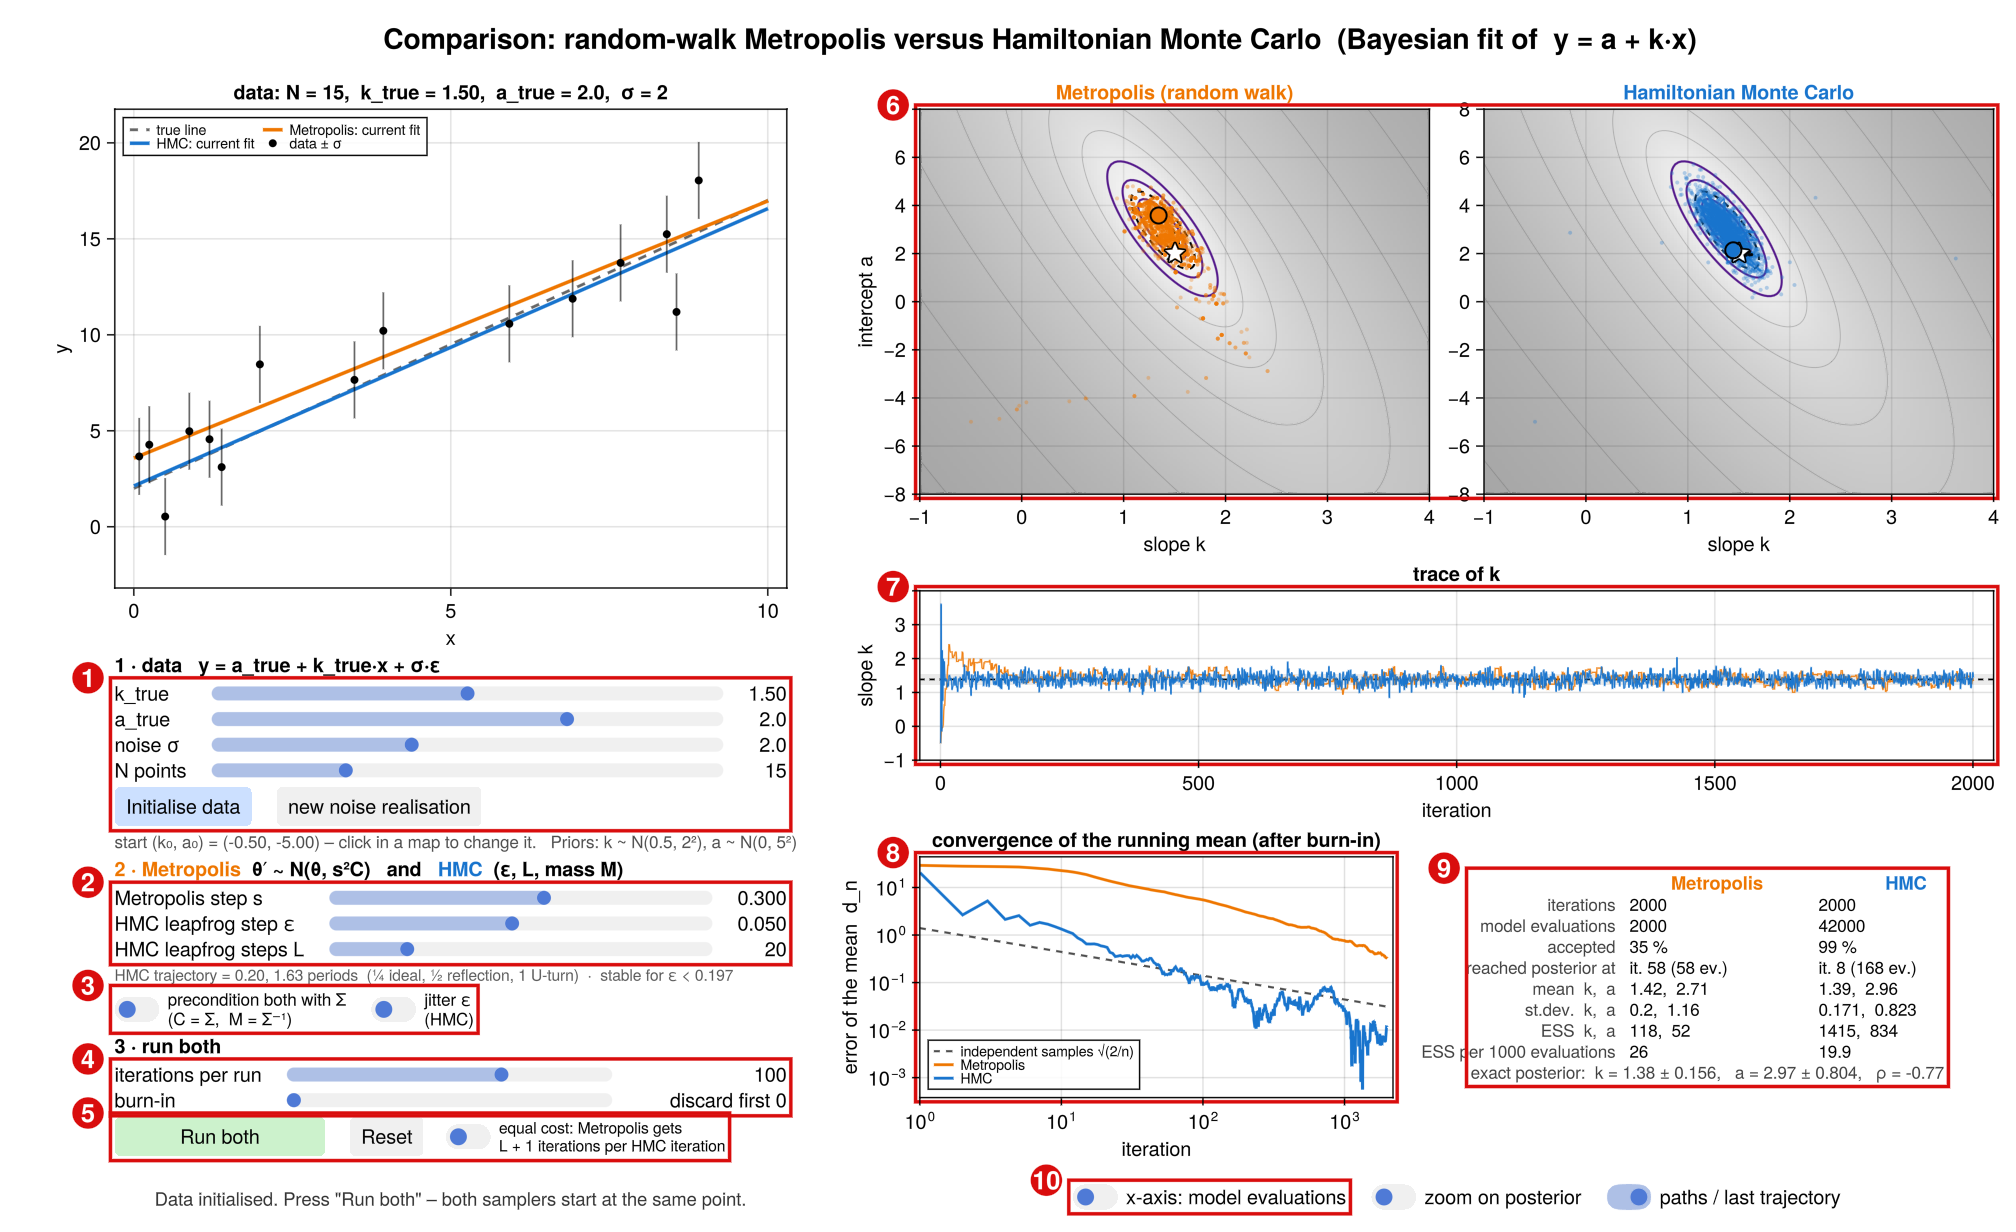
\includegraphics[width=\textwidth]{figures/cmp_overview.png}
\caption{Program 6 after 2000 iterations of each sampler (Metropolis $s=0.3$, HMC $\varepsilon=0.05$, $L=20$, no
preconditioning). Per iteration HMC is far ahead: it reaches the posterior after 8 iterations (Metropolis 58),
its running mean follows the ideal $\sqrt{2/n}$ line, and its ESS is 1415 and 834 against 118 and 52. But these
2000 HMC iterations cost 42\,000 gradient evaluations: per 1000 evaluations HMC gives 19.9 effective samples,
Metropolis 26.}
\label{fig:cmp}
\end{figure}

\paragraph{Step by step} (numbers as in Fig.~\ref{fig:cmp})
\begin{enumerate}[label=\protect\step{\arabic*}]
\item Data and \btn{Initialise data}. A click in either map sets the common starting point.
\item The Metropolis step $s$ and the HMC parameters $\varepsilon$ and $L$ (with the trajectory/stability note
  of Program~5 below).
\item \ctl{precondition both with $\Sigma$}: Metropolis uses $C=\Sigma$, HMC $M=\Sigma^{-1}$ (the exact posterior
  covariance, as if learned in a pilot run). This removes the correlation for both and compares them at their
  best; try $s\approx1.5$, $\varepsilon\approx0.3$, $L\approx5$. \ctl{jitter $\varepsilon$} as in Program~5.
\item Iterations per run and burn-in.
\item \btn{Run both}, \btn{Reset} (every reset is a new random realisation) and \ctl{equal cost}: Metropolis
  then gets $L+1$ iterations for each HMC iteration, so that both use the same number of model evaluations.
\item The two chains on the misfit map (HMC: last trajectory in black).
\item The trace of $k$ for both.
\item Convergence: the error of the running mean after burn-in,
  $d_n=\sqrt{(\hat m_n-m)^T\Sigma^{-1}(\hat m_n-m)}$ in units of the posterior; independent samples give
  $\approx\sqrt{2/n}$ (dashed), a chain with ESS effective samples $\approx\sqrt{2/\text{ESS}}$.
\item The comparison table: iterations, model evaluations, acceptance, first iteration inside the 99.7\,\%
  region, means and standard deviations, ESS and ESS per 1000 model evaluations.
\item \ctl{x-axis: model evaluations}: trace and convergence against the computing cost instead of the
  iteration number.
\end{enumerate}

\begin{figure}[H]
\centering
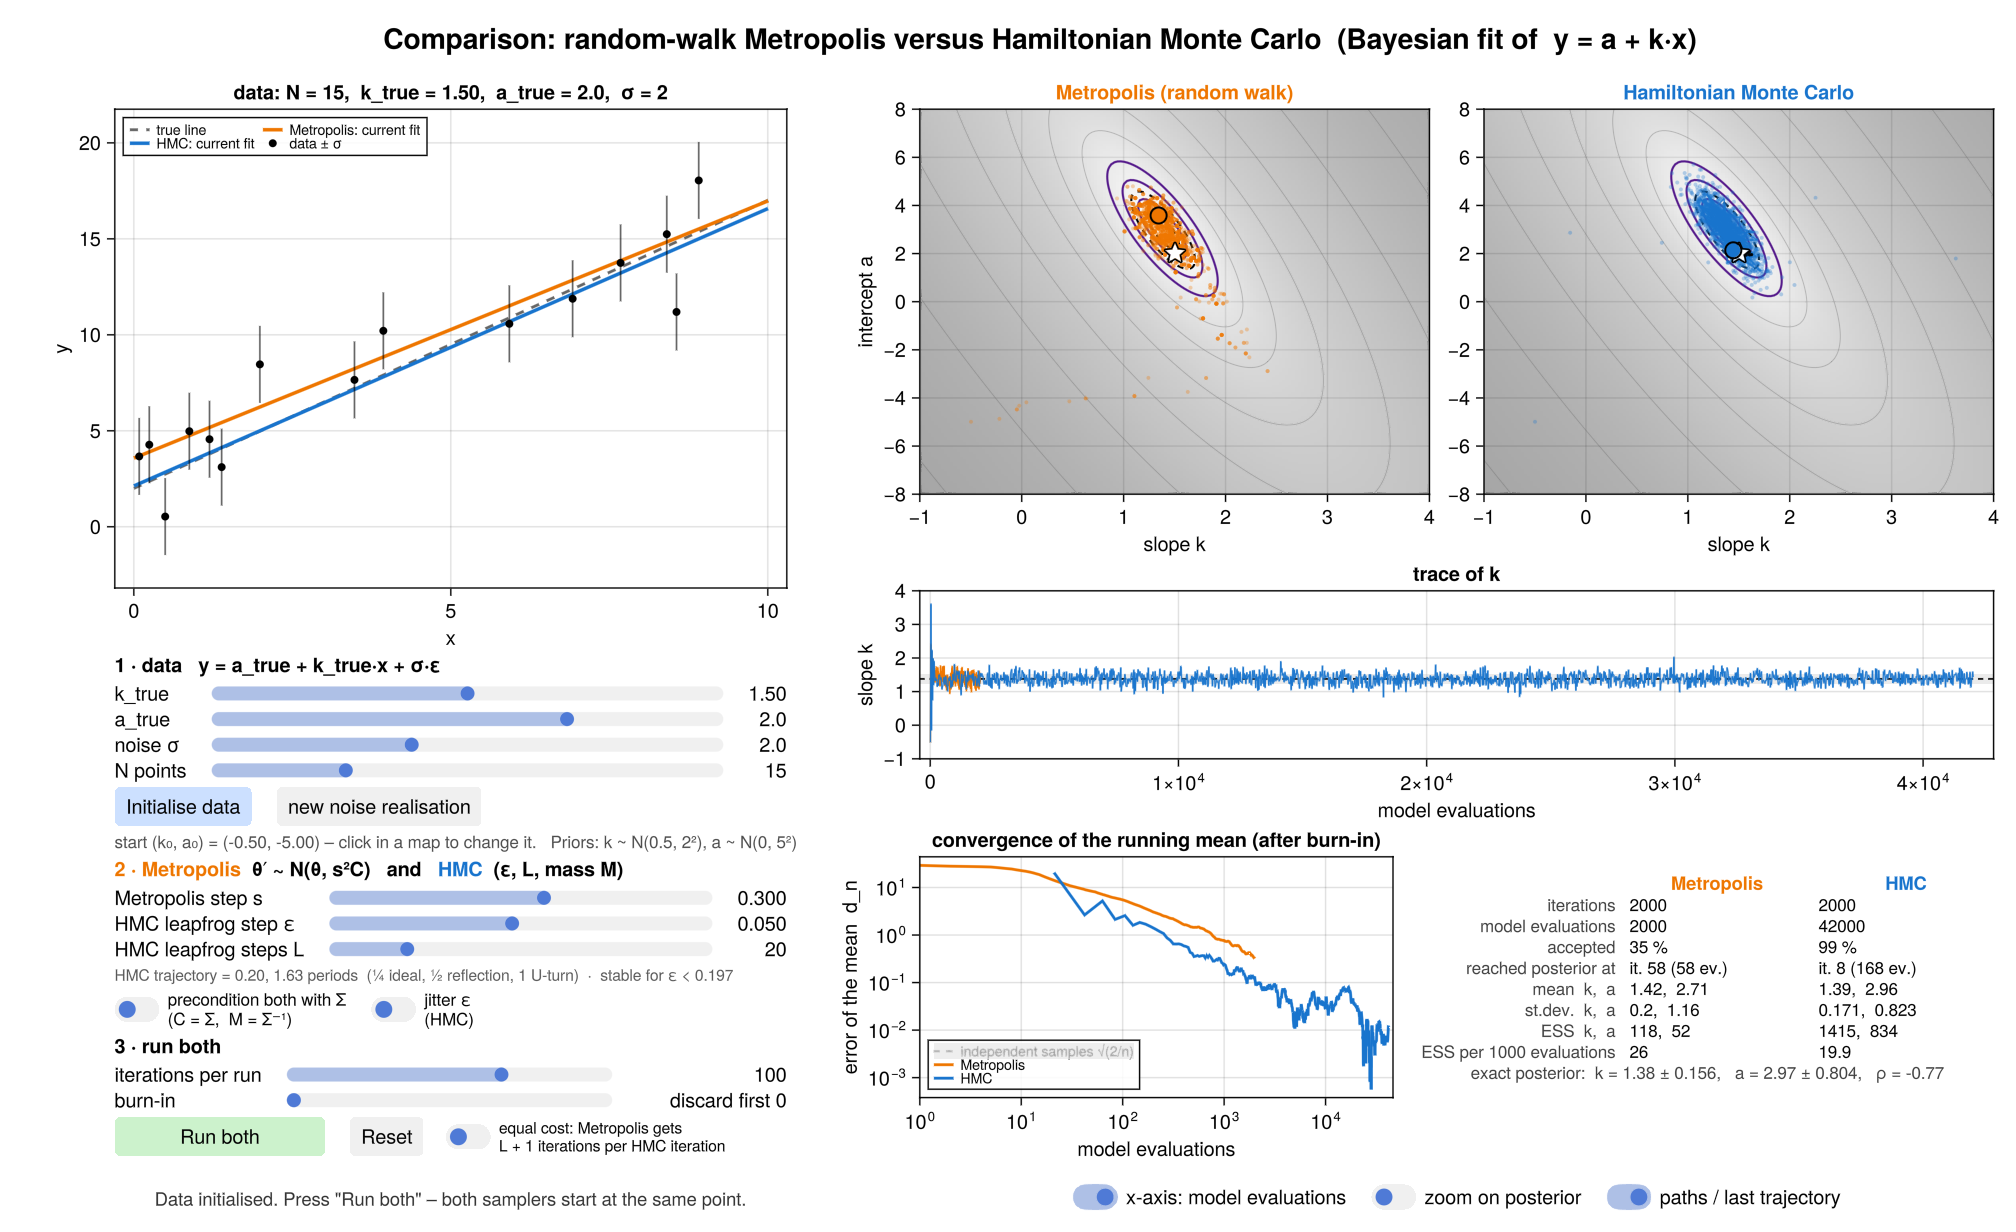
\includegraphics[width=0.49\textwidth]{figures/cmp_cost.png}\hfill
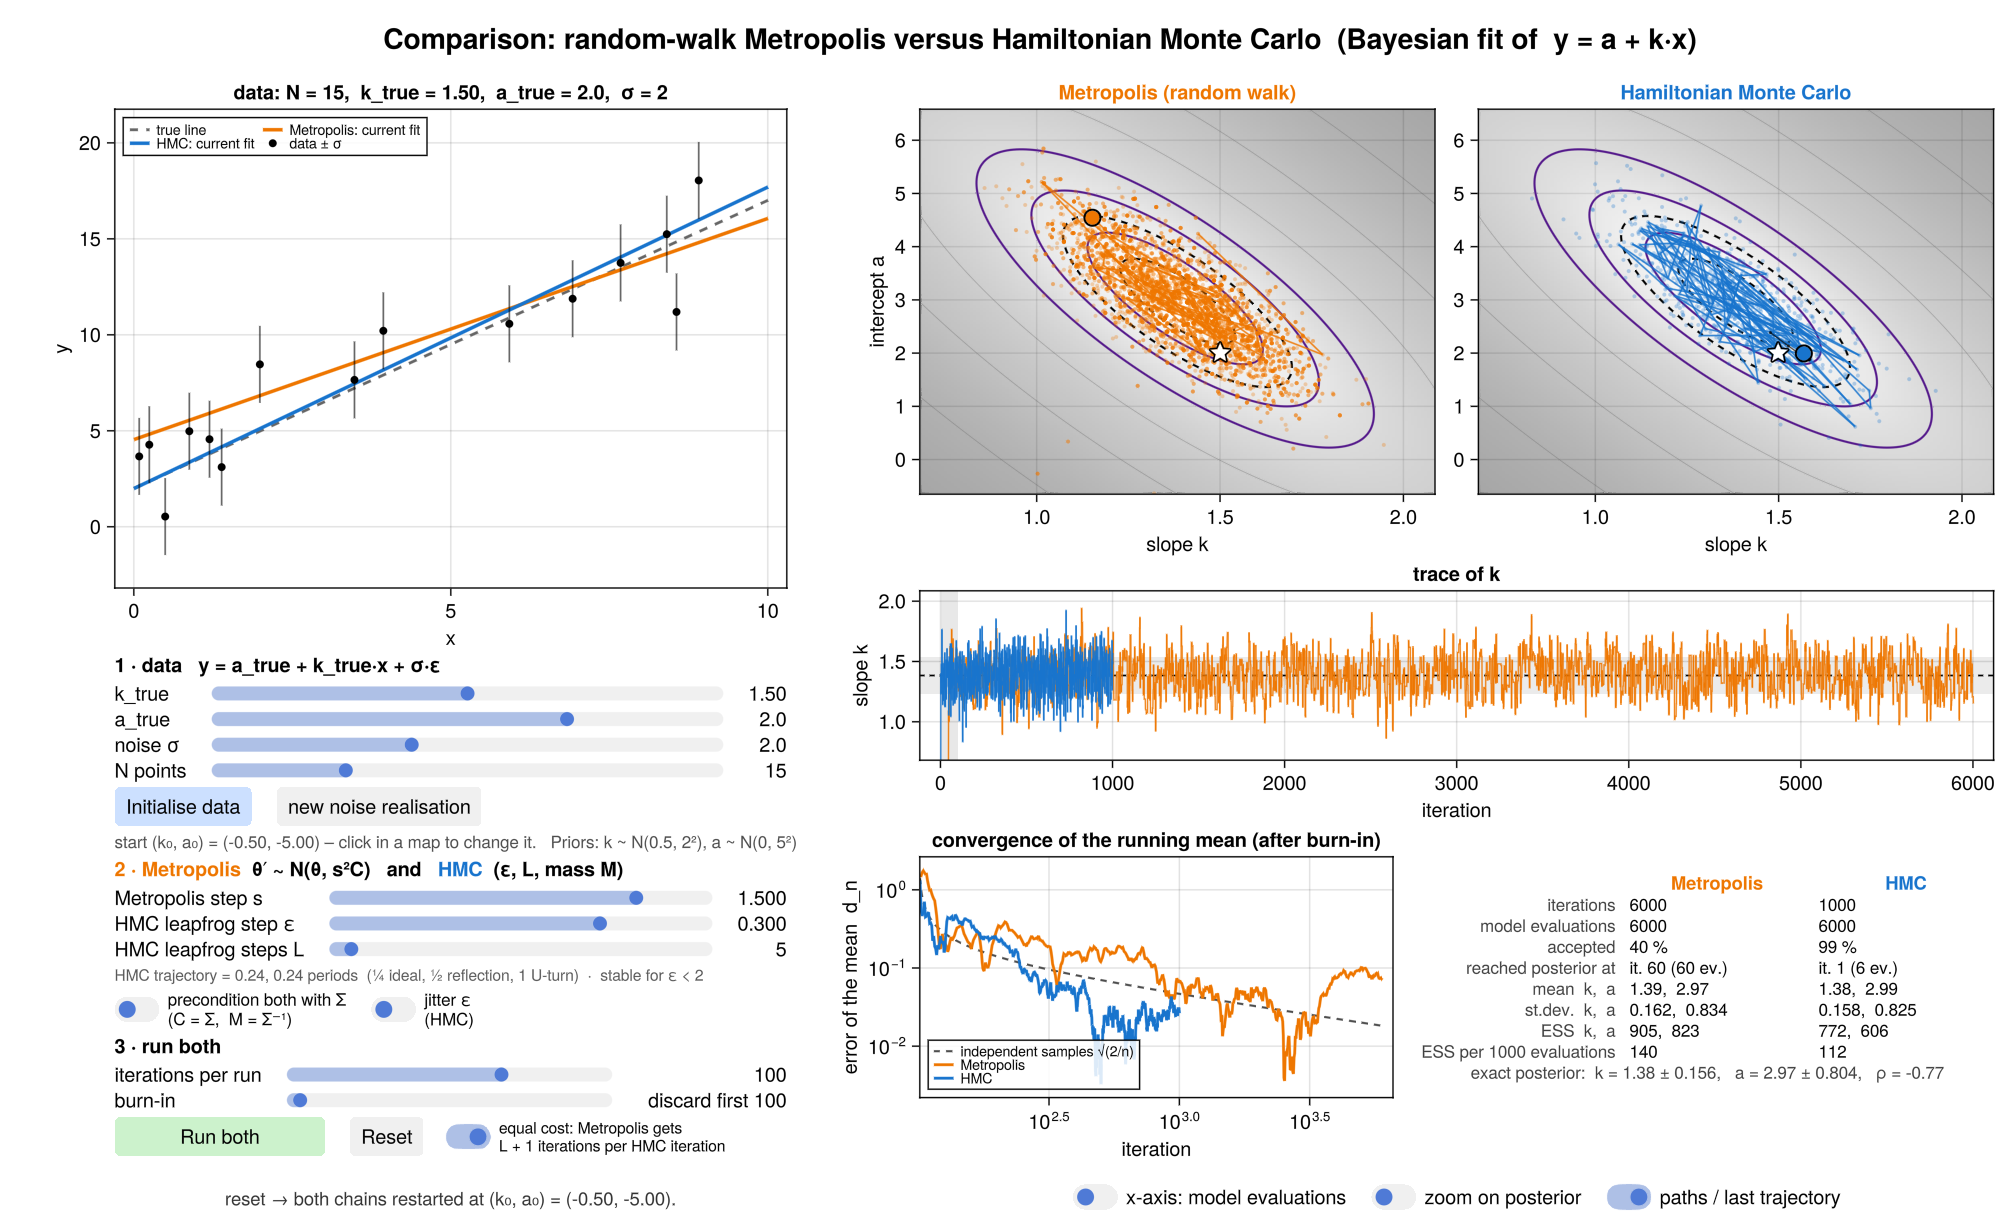
\includegraphics[width=0.49\textwidth]{figures/cmp_precond.png}
\caption{Left: the run of Fig.~\ref{fig:cmp} against model evaluations. The two convergence curves now lie on top
of each other: the Metropolis chain ends after 2000 evaluations, HMC continues to 42\,000. Right: preconditioned
($s=1.5$, $\varepsilon=0.3$, $L=5$), equal cost (Metropolis 6000 iterations, HMC 1000 iterations, 6000
evaluations each), burn-in 100. HMC is in the posterior after one iteration; both give correct statistics; ESS
per 1000 evaluations: Metropolis 140, HMC 112.}
\end{figure}

\subsection{Who converges faster?}
\begin{table}[H]
\centering\small
\caption{Effective samples per 1000 model evaluations, measured with Program~6 (two parameters, default data,
runs of a few thousand iterations; the numbers vary by $\pm30\,\%$ from run to run).}\label{tab:cmp}
\begin{tabular}{@{}lcc@{}}
\toprule
settings & Metropolis & HMC \\
\midrule
no preconditioning; $s=0.3$; $\varepsilon=0.05$, $L=20$ & 23--26 & 20--29 \\
no preconditioning; HMC $\varepsilon=0.1$, $L=15$         & 23     & 62 \\
preconditioned; $s=1.5$; $\varepsilon=0.3$, $L=5$         & 140--146 & 112--151 \\
preconditioned; HMC $\varepsilon=0.5$, $L=3$              & 146    & 232 \\
\midrule
effective samples per \emph{iteration}                    & 0.02--0.15 & 0.6--1 \\
\bottomrule
\end{tabular}
\end{table}
\begin{keypoint}
\begin{itemize}[leftmargin=*]
\item \textbf{Per iteration} HMC wins by a large factor (6 to 40 here): each trajectory travels far and is almost
  always accepted; it also reaches the posterior from a poor start in a few iterations.
\item \textbf{Per model evaluation}, i.e.\ per unit of computing time, the two are of \emph{similar}
  efficiency for two parameters; depending on the tuning and on the random run either can win. The most
  important improvement for both is the same: a proposal (or mass matrix) adapted to the shape of the posterior,
  which increases the efficiency of both by a factor of about six.
\item \textbf{The difference grows with the number of parameters $D$.} To keep a reasonable acceptance, the step
  of a random walk must shrink as $D^{-1/2}$, and it needs $O(D)$ iterations per independent sample; the
  leapfrog step of HMC only as $D^{-1/4}$ (Neal, 2011; Beskos et al., 2013). With hundreds or thousands of
  parameters (e.g.\ a discretised profile, a tomographic model, a hierarchical model) HMC is faster by orders
  of magnitude, provided the gradient is available, which is why modern probabilistic programming tools
  (Stan, Turing.jl, PyMC) are built on HMC/NUTS. Program~7 (Section~\ref{sec:cmp2}) measures this trend for up to
  ten parameters.
\item Both need care: burn-in and step size for Metropolis; step size, trajectory length (U-turns, resonances)
  and divergences for HMC. Always look at the traces, and run more than one chain.
\end{itemize}
\end{keypoint}

\begin{tryit}
\begin{itemize}
\item Switch \ctl{x-axis: model evaluations} on and off for the default settings. Which sampler ``wins''?
\item Switch \ctl{equal cost} on and compare the convergence curves on the same cost axis.
\item Precondition both and tune each sampler to its best ESS per 1000 evaluations. How close are they?
\item Set the burn-in to 0 and look at the convergence plot: how long does the starting point bias the
  running mean of each sampler?
\item Choose an HMC resonance ($\varepsilon=0.15$, $L=20$, no preconditioning): which of the measures in the
  table reveal the problem, and which do not?
\end{itemize}
\end{tryit}

%==============================================================================
\clearpage
\section{Program 7 – Metropolis and HMC with many parameters}\label{sec:cmp2}
%==============================================================================
\textbf{File:} \file{Comparison\_MCMC\_to\_HMC\_2.jl}.\quad The question left open in Section~\ref{sec:cmp}: how
do the two samplers behave when the number of parameters grows? The model is a polynomial with $D=1\dots10$
coefficients on $-1\le x\le1$,
\begin{equation}
  y = \sum_{j=0}^{D-1} c_j\,\varphi_j(x),\qquad c_j\sim\mathcal{N}(0,2^2),
\end{equation}
with either the \textbf{Legendre polynomials} $\varphi_j=P_j(x)$, which are nearly orthogonal for data spread over
$[-1,1]$ (the coefficients are almost uncorrelated), or the \textbf{monomials} $\varphi_j=x^j$, whose
coefficients are strongly correlated. The model is linear in the $c_j$, so the posterior is again an exact
Gaussian: $U(\mathbf c)=\tfrac12\mathbf c^T\Lambda\mathbf c-\mathbf h^T\mathbf c$, with
$\Lambda=\Phi^T\Phi/\sigma^2+I/\sigma_p^2$, mean $\Lambda^{-1}\mathbf h$ and covariance $\Sigma=\Lambda^{-1}$.

Both samplers can be \textbf{tuned optimally} for every $D$, using the theory of Sections~\ref{sec:practical}
and~\ref{sec:osc} for a Gaussian target with frequencies $\omega$ ($\omega^2$ = eigenvalues of $C\Lambda$; all
$\omega=1$ when preconditioned with $C=\Sigma$):
\begin{equation}
  \text{Metropolis: } s=\frac{2.38}{\sqrt{D}\,\omega_\text{max}},\qquad
  \text{HMC: } \varepsilon=\frac{0.8\,D^{-1/4}}{\omega_\text{max}},\quad
  L=\text{round}\Bigl(\frac{\pi/2}{\omega_\text{min}\,\varepsilon}\Bigr)\ \ \text{(a quarter period)}.
\end{equation}
The step of the random walk must shrink as $D^{-1/2}$ to keep a reasonable acceptance, the leapfrog step only as
$D^{-1/4}$; this is the origin of the different scaling of the two methods.

\begin{figure}[H]
\centering
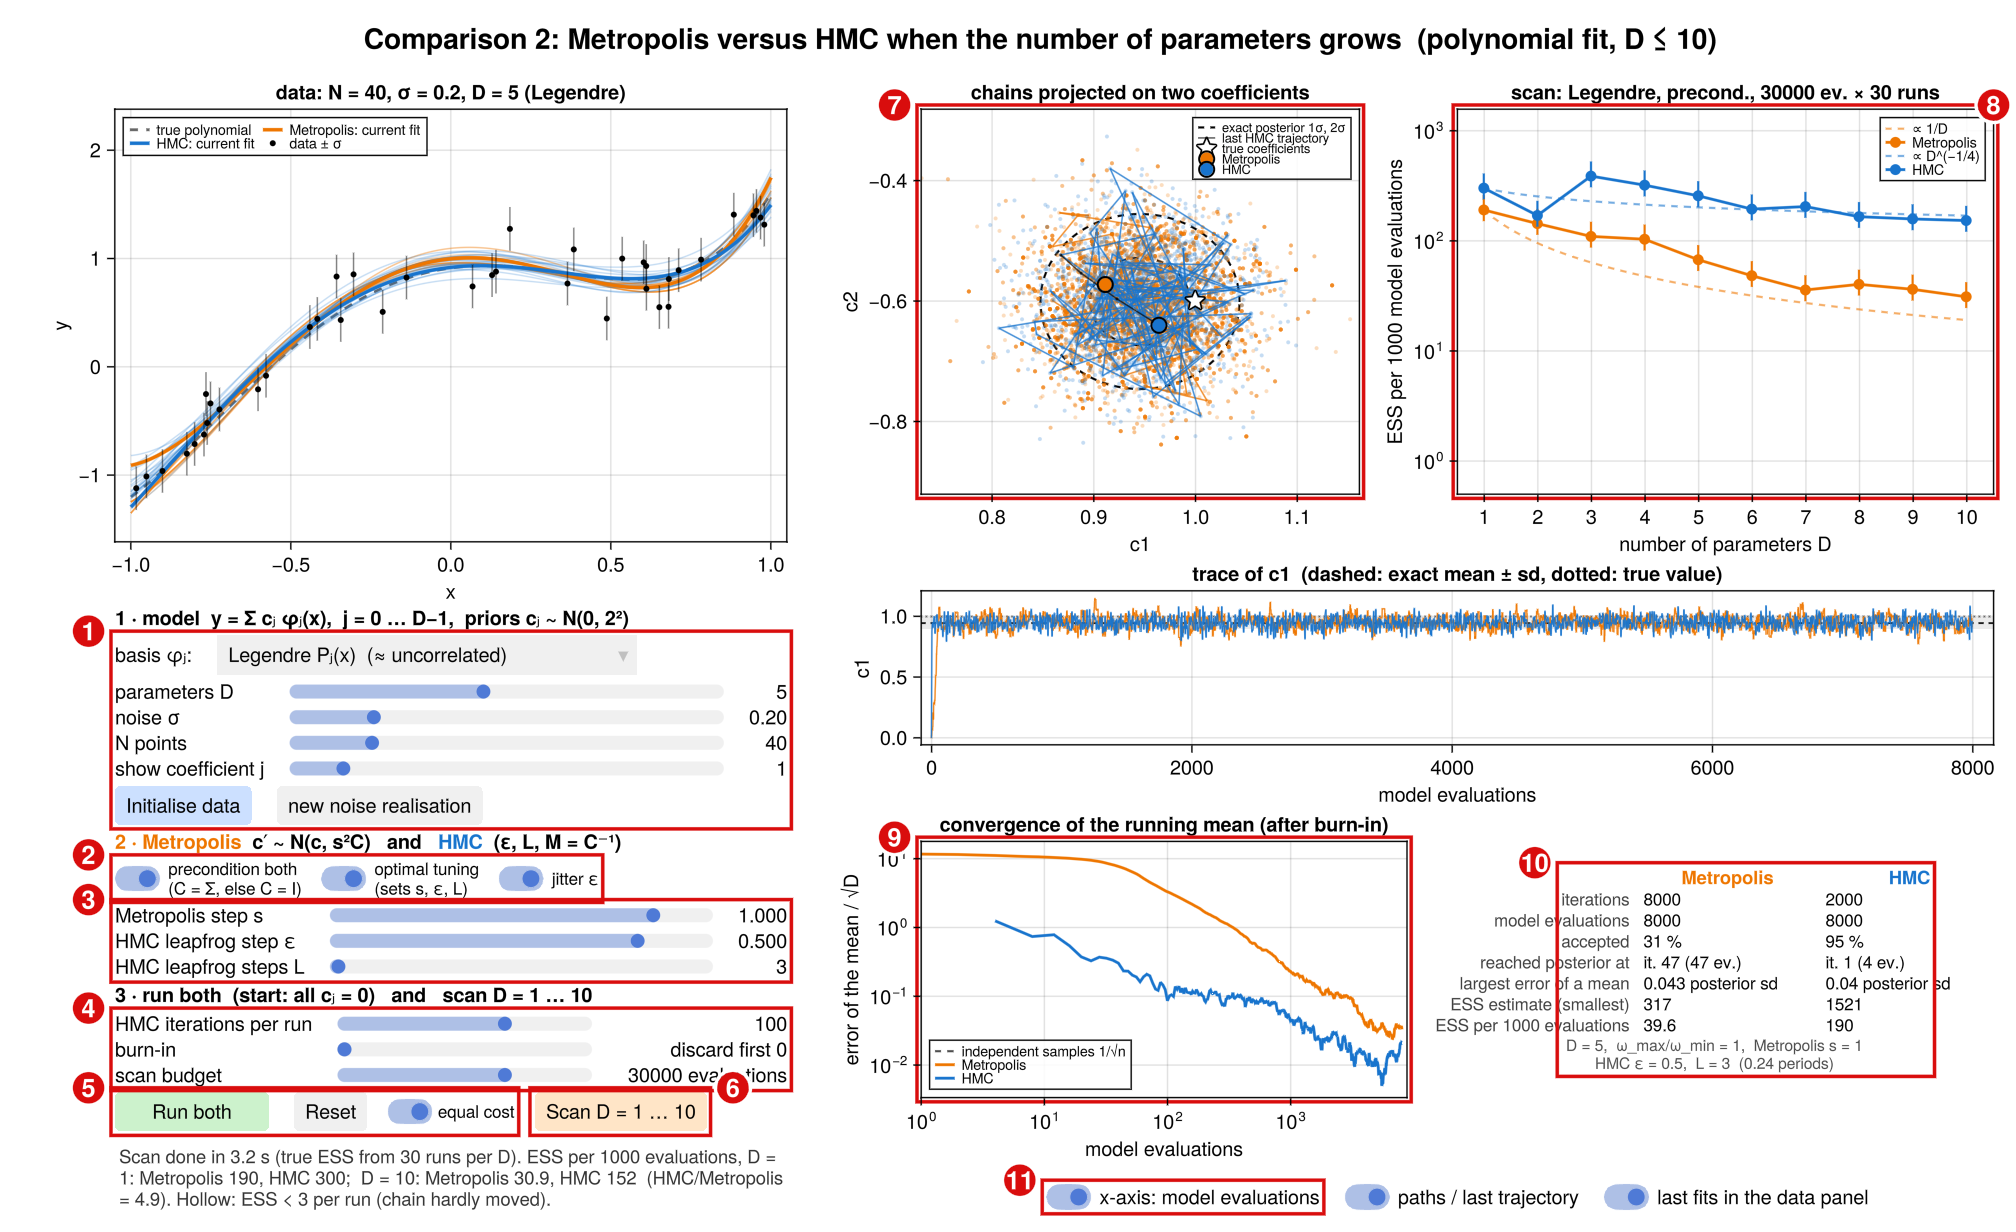
\includegraphics[width=\textwidth]{figures/cmp2_overview.png}
\caption{Program 7 with $D=5$ Legendre coefficients, preconditioned and optimally tuned, after a scan and 2000
HMC iterations (8000 Metropolis iterations, equal cost). Upper right: the scan. At $D=1$ the two samplers are
similar (Metropolis 190, HMC 300 effective samples per 1000 evaluations); at $D=10$ Metropolis has dropped to 31,
following the dashed $1/D$ line, HMC only to 152, close to the $D^{-1/4}$ line: a factor of 4.9 in favour of
HMC.}
\label{fig:cmp2}
\end{figure}

\paragraph{Step by step} (numbers as in Fig.~\ref{fig:cmp2})
\begin{enumerate}[label=\protect\step{\arabic*}]
\item The model and the data: the basis (Legendre or monomials), the number of parameters $D$ (changing it
  creates a new problem and restarts the chains), the noise, the number of points, and the coefficient $j$ shown
  in the projection and the trace. \btn{Initialise data}, \btn{new noise realisation}.
\item \ctl{precondition both} ($C=\Sigma$ for Metropolis, $M=\Sigma^{-1}$ for HMC; otherwise $C=I$),
  \ctl{optimal tuning} (sets $s$, $\varepsilon$ and $L$ for every $D$; moving one of these sliders switches it
  off) and \ctl{jitter $\varepsilon$}.
\item The Metropolis step $s$, the leapfrog step $\varepsilon$ and the number of leapfrog steps $L$.
\item HMC iterations per run, burn-in, and the budget of model evaluations per run of the scan.
\item \btn{Run both} (start: all $c_j=0$), \btn{Reset} and \ctl{equal cost} (on by default: Metropolis gets
  $L+1$ iterations per HMC iteration).
\item \btn{Scan D = 1 … 10}: for every $D$ both samplers are run 30 times with the optimal settings and the
  chosen budget, each run starting from an exact posterior draw; the \emph{true} effective sample size follows
  from the error of the sample means (Section~\ref{sec:numerics}). About 3\,s.
\item The two chains projected on the coefficients $c_j$ and $c_{j+1}$, with the exact 1$\sigma$/2$\sigma$
  ellipses and the last HMC trajectory.
\item The scan: effective samples per 1000 model evaluations against $D$, with $\approx68\,\%$ uncertainty bars
  and the trends $\propto1/D$ and $\propto D^{-1/4}$ (dashed, through the value at $D=1$). Hollow markers: fewer
  than 3 effective samples per run; the chain hardly moved.
\item The error of the running mean in units of the posterior, divided by $\sqrt{D}$ (independent samples:
  $1/\sqrt n$).
\item The comparison table for the run on the left; its ESS is the quick batch-means \emph{estimate}. Below it the
  settings: $D$, the conditioning $\omega_\text{max}/\omega_\text{min}$, $s$, $\varepsilon$, $L$ and the trajectory
  length in periods.
\item \ctl{x-axis: model evaluations} (on by default): trace and convergence against the computing cost.
\end{enumerate}

\begin{figure}[H]
\centering
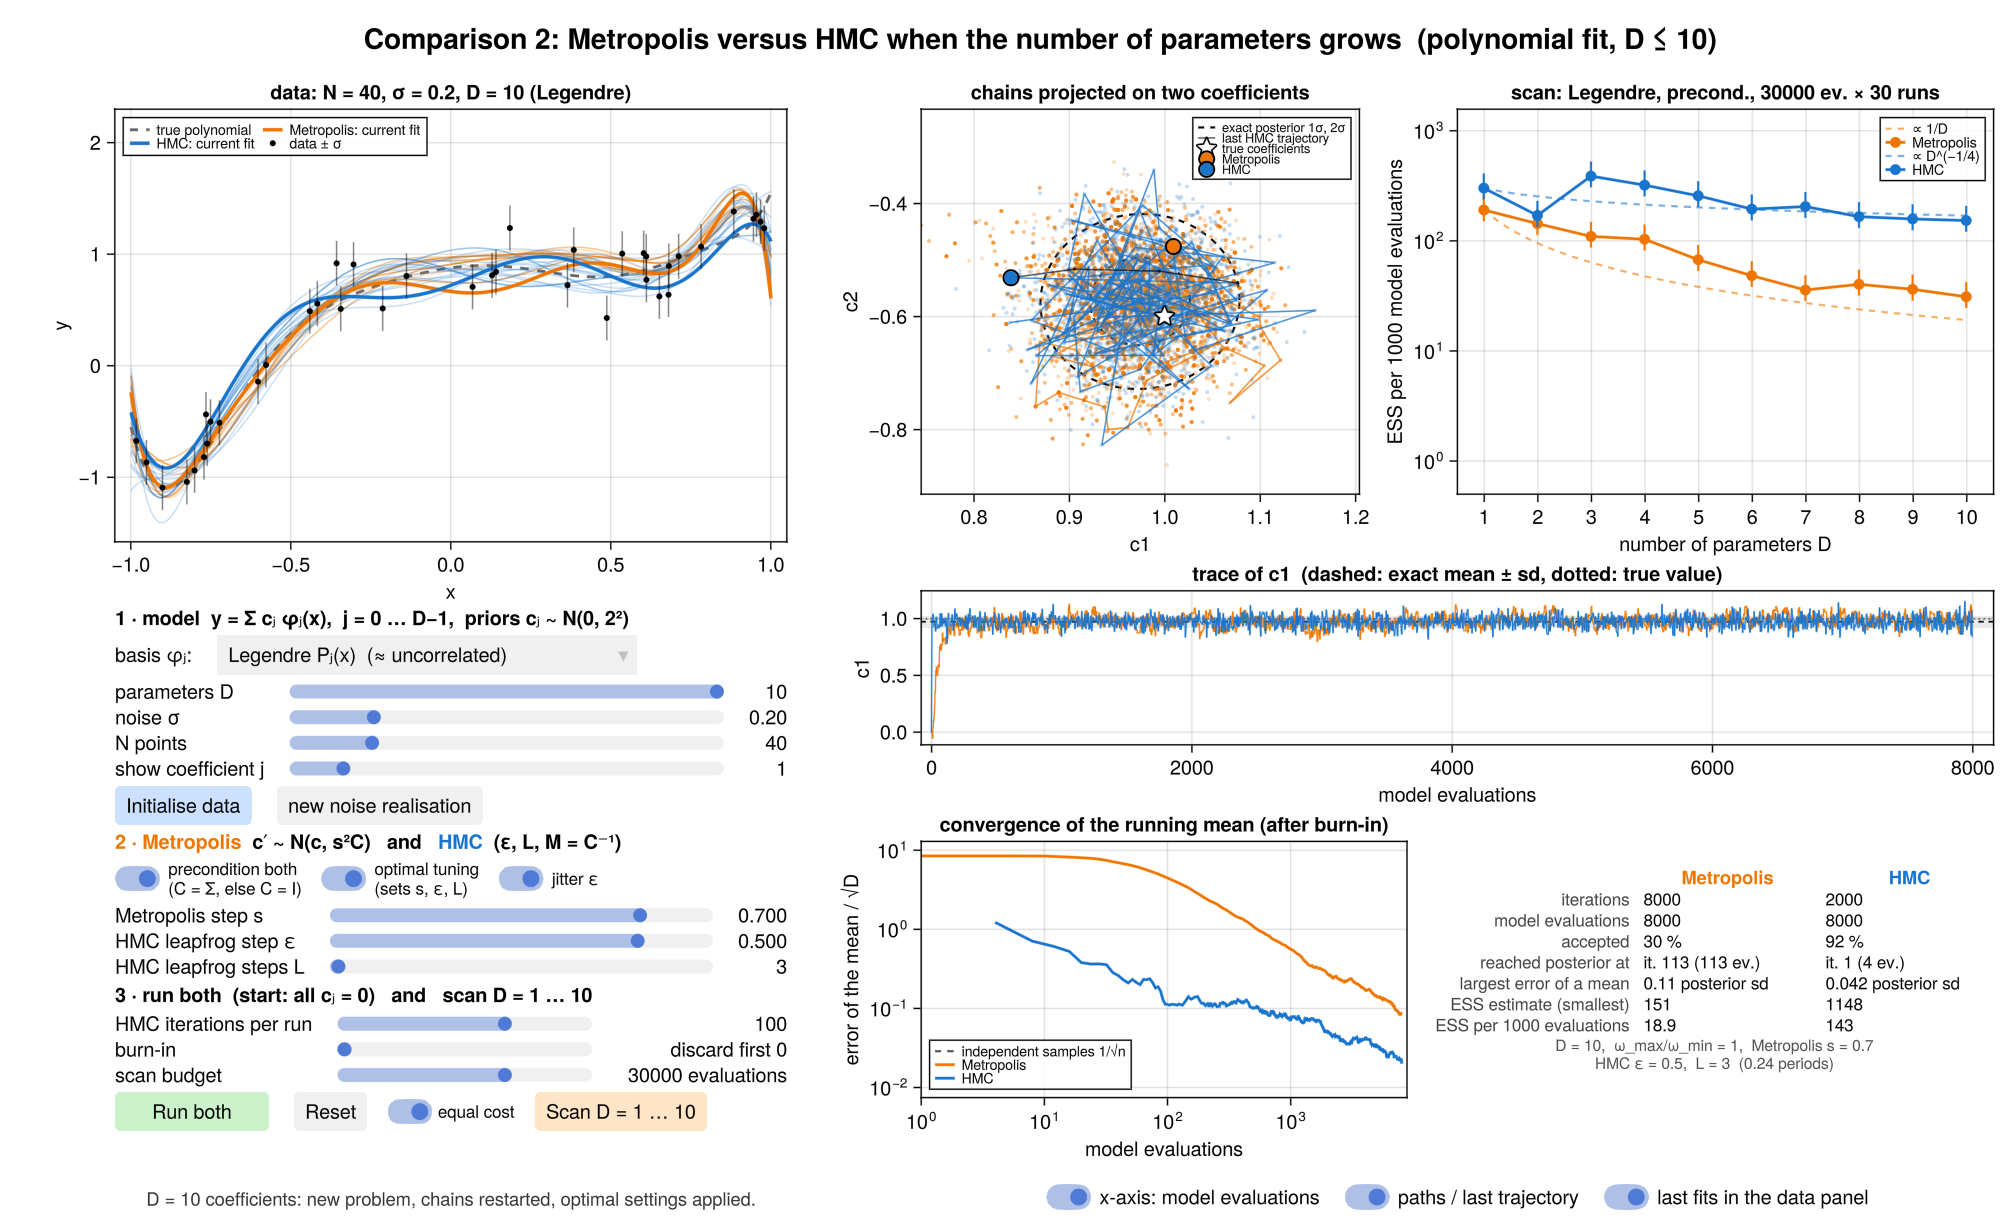
\includegraphics[width=0.49\textwidth]{figures/cmp2_D10.png}\hfill
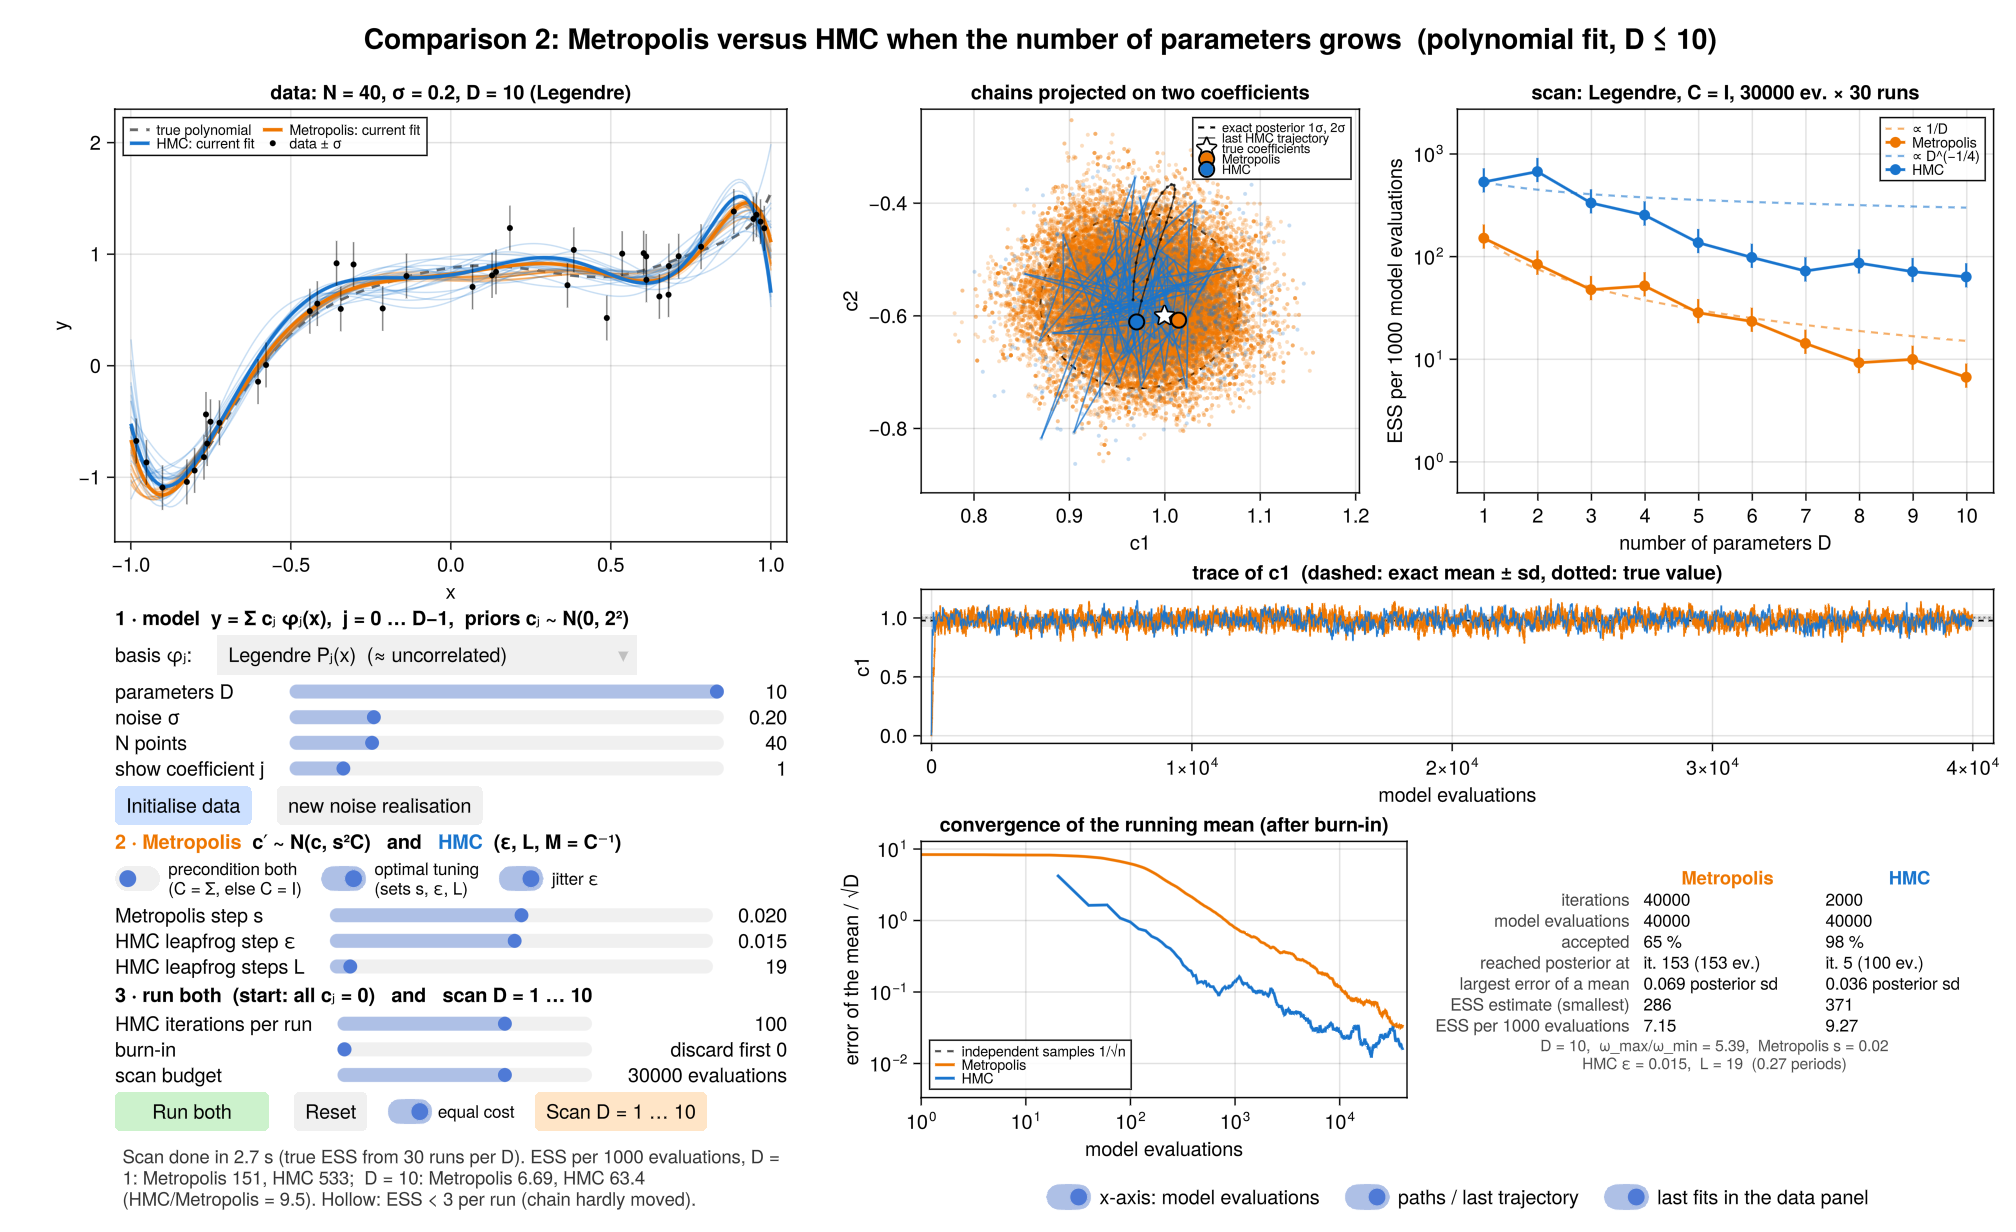
\includegraphics[width=0.49\textwidth]{figures/cmp2_legendre_noprecond.png}
\caption{Left: $D=10$, Legendre, preconditioned, 8000 evaluations each. HMC ($\varepsilon=0.5$, $L=3$) reaches
the posterior in its first iteration, Metropolis ($s=0.7$, 30\,\% accepted) after 113; the largest error of a
posterior mean is 0.04 posterior standard deviations for HMC, 0.11 for Metropolis. Right: the same problem
\emph{without} preconditioning ($C=I$). The coefficients now have different posterior widths
($\omega_\text{max}/\omega_\text{min}=5.4$), the step of Metropolis is set by the narrowest one ($s=0.02$), HMC needs
$L=19$ steps of $\varepsilon=0.015$. Scan: Metropolis drops from 151 to 6.7, HMC from 533 to 63 effective samples
per 1000 evaluations, a factor of 9.5 at $D=10$.}
\end{figure}

\begin{figure}[H]
\centering
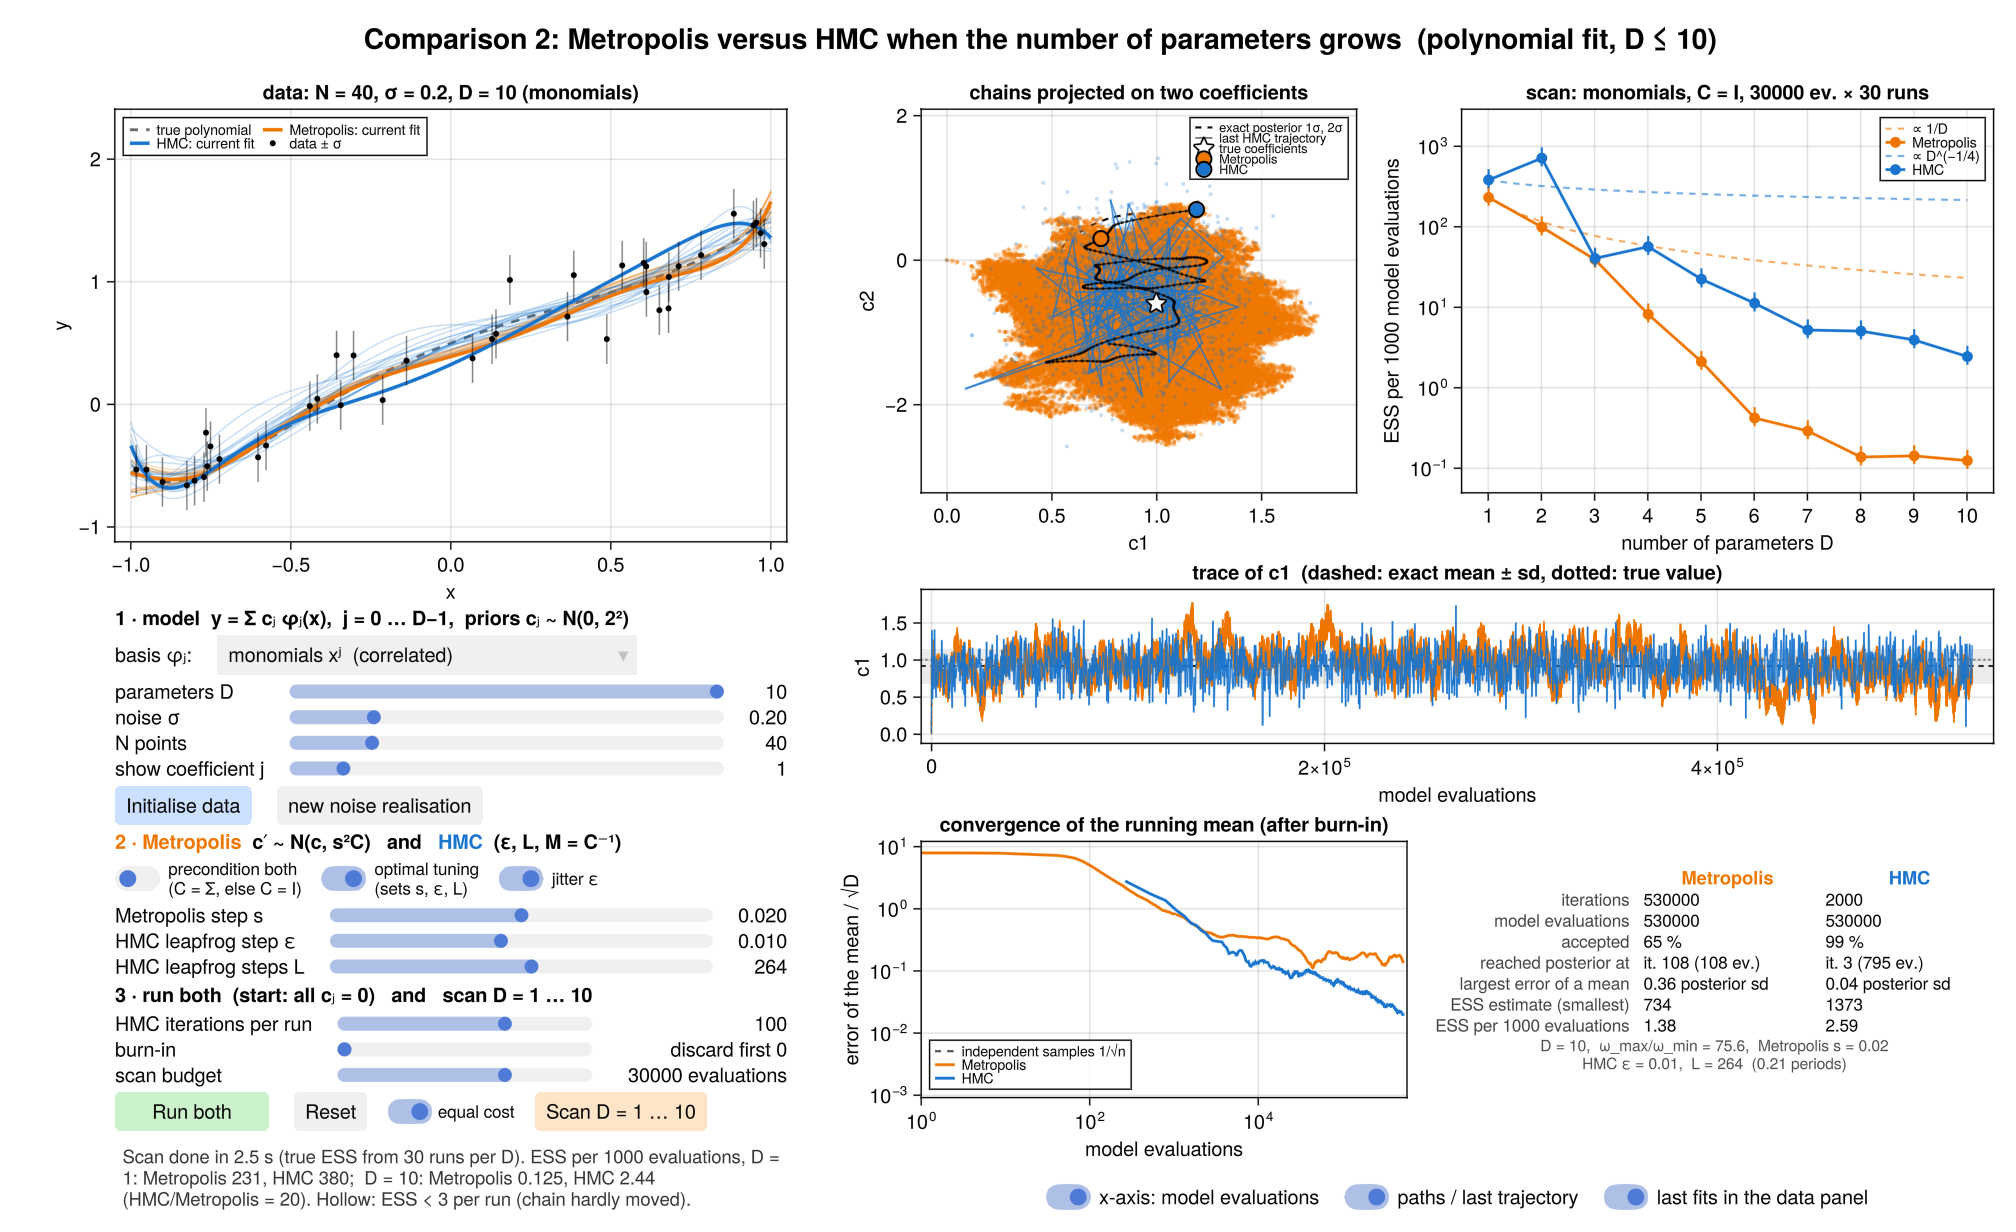
\includegraphics[width=0.75\textwidth]{figures/cmp2_monomial_noprecond.png}
\caption{Monomial basis without preconditioning: a badly conditioned posterior ($\omega_\text{max}/\omega_\text{min}
=76$ at $D=10$). Scan: Metropolis collapses from 231 to 0.13 effective samples per 1000 evaluations, HMC from 380 to
2.4, a factor of 20. In the run on the left (530\,000 evaluations each; HMC with $L=264$, its last trajectory
winds through the posterior in black) the orange cloud of Metropolis covers the posterior, and the trace looks
acceptable, but its running mean stalls: the largest error of a mean is 0.36 posterior standard deviations
(HMC: 0.04). The table estimates 1.38 effective samples per 1000 evaluations for Metropolis, eleven times the true
value of the scan, 0.13.}
\end{figure}

\begin{table}[H]
\centering\small
\caption{True effective samples per 1000 model evaluations measured by the scan (30\,000 evaluations per run, 30
runs per $D$; the values scatter by about $\pm30\,\%$ between scans).}\label{tab:cmp2}
\begin{tabular}{@{}lccccc@{}}
\toprule
& \multicolumn{2}{c}{Metropolis} & \multicolumn{2}{c}{HMC} & HMC/Metropolis \\
\cmidrule(lr){2-3}\cmidrule(lr){4-5}
& $D=1$ & $D=10$ & $D=1$ & $D=10$ & at $D=10$ \\
\midrule
preconditioned (Legendre or monomials) & 190--230 & 30--35 & 300--380 & 150--220 & 4--7 \\
Legendre, $C=I$                        & 150--300 & 7      & 530--640 & 50--65   & 7--10 \\
monomials, $C=I$                       & 230--270 & 0.1    & 350--430 & 2.4--3.3 & 20--30 \\
\bottomrule
\end{tabular}
\end{table}

\begin{keypoint}
\begin{itemize}[leftmargin=*]
\item With one parameter the two samplers are similar per unit of computing work. With every additional
  parameter random-walk Metropolis loses a factor $\approx1/D$, HMC only $\approx D^{-1/4}$; at $D=10$ HMC is
  already 4--7 times more efficient in the best case. Extrapolating the two trends: about 15 times at $D=100$,
  about 100 times at $D=1000$.
\item Correlated parameters (a badly conditioned posterior) hurt both, Metropolis much more: its step is limited
  by the narrowest direction of the posterior, and it then crawls along the widest one. Preconditioning with the
  posterior covariance (learned in a pilot run) makes both samplers independent of the parametrisation:
  Legendre and monomials then give the same efficiency.
\item Do not trust a quick ESS estimate for a chain that mixes badly: here the batch-means estimate was too
  optimistic by a factor of 11 (and up to 200 in shorter runs). Long runs, several independent chains and a look at
  the running mean are the safer check.
\end{itemize}
\end{keypoint}

\begin{tryit}
\begin{itemize}
\item Run the scan for all four combinations of basis and preconditioning. In which case does the advantage of
  HMC grow fastest with $D$?
\item Preconditioned: compare the scans for the Legendre and the monomial basis. Why are they the same within the
  uncertainty?
\item Choose $D=10$, switch \ctl{optimal tuning} off and increase $\varepsilon$ in steps. At what $\varepsilon$
  does the acceptance of HMC drop, and what happens to the efficiency? Do the same for the Metropolis step $s$.
\item Switch \ctl{equal cost} off and \ctl{x-axis: model evaluations} off: per iteration, how large is the
  advantage of HMC at $D=10$? Why is this comparison unfair?
\item Monomials without preconditioning at $D=10$: run until 500\,000 evaluations and compare the ESS of the
  table with the value of the scan.
\end{itemize}
\end{tryit}

%==============================================================================
\section{Troubleshooting}
%==============================================================================
\begin{itemize}
\item \textbf{No window opens / OpenGL error}: GLMakie needs a graphics card with OpenGL 3.3. On a remote
  machine without a display use the programs locally.
\item \textbf{The first start takes long}: this is the compilation of GLMakie (once per Julia session).
\item \textbf{The window is too small}: the controls always stay visible; the data panel shrinks first. Below
  about $1280\times680$ pixels the layout becomes cramped.
\item \textbf{The data sliders have no effect}: press \btn{Initialise data}.
\item \textbf{The histogram does not match the exact posterior}: not enough samples, burn-in not removed, the
  Hastings correction switched off (Program~2, 3), or an HMC resonance or U-turn (Programs 4--7).
\item \textbf{The scan of Program 7 takes a few seconds}: it runs $2\times10\times30$ chains; with the budget
  $10^5$ evaluations about 10\,s.
\item \textbf{Screenshots for this guide}: every figure in \file{guide/figures} is rebuilt by
\begin{lstlisting}
julia guide/make_screenshots.jl all     # each program in its own process
julia guide/make_screenshots.jl hmc1    # one: mcmc1..3, hmc1, hmc2, cmp, cmp2
\end{lstlisting}
\end{itemize}

%==============================================================================
\section*{References}
\addcontentsline{toc}{section}{References}
%==============================================================================
\begin{itemize}[leftmargin=*,label={}]
\item Beskos, A., Pillai, N., Roberts, G., Sanz-Serna, J.-M., Stuart, A. (2013). Optimal tuning of the hybrid
  Monte Carlo algorithm. \emph{Bernoulli} 19, 1501--1534.
\item Betancourt, M. (2017). A conceptual introduction to Hamiltonian Monte Carlo. arXiv:1701.02434.
\item Duane, S., Kennedy, A.\,D., Pendleton, B.\,J., Roweth, D. (1987). Hybrid Monte Carlo. \emph{Physics
  Letters B} 195, 216--222.
\item Gelman, A., Carlin, J.\,B., Stern, H.\,S., Dunson, D.\,B., Vehtari, A., Rubin, D.\,B. (2013).
  \emph{Bayesian Data Analysis}, 3rd ed. CRC Press.
\item Hastings, W.\,K. (1970). Monte Carlo sampling methods using Markov chains and their applications.
  \emph{Biometrika} 57, 97--109.
\item Hoffman, M.\,D., Gelman, A. (2014). The No-U-Turn Sampler: adaptively setting path lengths in Hamiltonian
  Monte Carlo. \emph{Journal of Machine Learning Research} 15, 1593--1623.
\item Metropolis, N., Rosenbluth, A.\,W., Rosenbluth, M.\,N., Teller, A.\,H., Teller, E. (1953). Equation of
  state calculations by fast computing machines. \emph{Journal of Chemical Physics} 21, 1087--1092.
\item Mosegaard, K., Tarantola, A. (1995). Monte Carlo sampling of solutions to inverse problems.
  \emph{Journal of Geophysical Research} 100, 12431--12447.
\item Neal, R.\,M. (2011). MCMC using Hamiltonian dynamics. In: Brooks, S., Gelman, A., Jones, G., Meng, X.-L.
  (eds.), \emph{Handbook of Markov Chain Monte Carlo}, CRC Press, 113--162.
\item Roberts, G.\,O., Gelman, A., Gilks, W.\,R. (1997). Weak convergence and optimal scaling of random walk
  Metropolis algorithms. \emph{Annals of Applied Probability} 7, 110--120.
\item Tarantola, A. (2005). \emph{Inverse Problem Theory and Methods for Model Parameter Estimation}. SIAM.
\end{itemize}

\end{document}
